%%%%%%%%%%%%%%%%%%%%%%%%%%%%%%%%%%%%%%%%%%%%%%%%%%%%%%%%%%%%%%%%%%%%%%%%%%%%%%%%%%%%%%%%%%%%%%%%%%%%%
% This template is distributed with ABSOLUTELY NO WARRANTY.
% It serves as a guideline and constitutes a basic structure for a
% thesis/dissertation. The user assumes full responsibility for formatting
% and typesetting their document and for verifying that all the thesis
% requirements set by the University of Tennessee are met. Please refer to the most
% recent UT thesis guide (http://gradschool.utk.edu/thesesdissertations/formatting/)
% or contact the thesis consultant (http://gradschool.utk.edu/thesesdissertations/).
% Please report any bugs to the thesis consultant.
%%%%%%%%%%%%%%%%%%%%%%%%%%%%%%%%%%%%%%%%%%%%%%%%%%%%%%%%%%%%%%%%%%%%%%%%%%%%%%%%%%%%%%%%%%%%%%%%%%%%%
% O P T I O N S:
% 1. thesis/dissertation
% 2. monochrome
% 3. all options provided by the report class
%%%%%%%%%%%%%%%%%%%%%%%%%%%%%%%%%%%%%%%%%%%%%%%%%%%%%%%%%%%%%%%%%%%%%%%%%%%%%%%%%%%%%%%%%%%%%%%%%%%%%
%First, is this a thesis or dissertation? Choose one by commenting out the one you don't need:
%\documentclass[thesis,letterpaper,12pt]{utthesis} % thesis
\documentclass[dissertation,letterpaper,12pt]{utthesis} %dissertation
% some alternatives are:
%\documentclass[thesis,monochrome,letterpaper,12pt]{utthesis} %thesis, monochrome text
\renewcommand{\baselinestretch}{1.5} 	 % line Spacing
%%%%%%%%%%%%%%%%%%%%%%%%%%%%%%%%%%%%%%%%%%%%%%%%%%%%%%%%%%%%%%%%%%%%%%%%%%%%%%%%%%%%%%%%%%%%%%%%%%%%%
% TO DO: FILL IN YOUR INFORMATION BELOW - READ THIS SECTION CAREFULLY
%%%%%%%%%%%%%%%%%%%%%%%%%%%%%%%%%%%%%%%%%%%%%%%%%%%%%%%%%%%%%%%%%%%%%%%%%%%%%%%%%%%%%%%%%%%%%%%%%%%%%
\title{My Thesis or Dissertation Title}	       	% title of thesis/dissertation
\author{Cedric Landerer}                			% author's name
\copyrightYear{2018}            				% copyright year of your thesis/dissertation
\graduationMonth{December}           				% month of graduation for your thesis/dissertation
\degree{Doctor of Philosophy}	    			% degree: Doctor of Philosophy, Master of Science, Master of Engineering...
\university{The University  of Tennessee, Knoxville}	% school name
%%%%%%%%%%%%%%%%%%%%%%%%%%%%%%%%%%%%%%%%%%%%%%%%%%%%%%%%%%%%%%%%%%%%%%%%%%%%%%%%%%%%%%%%%%%%%%%%%%%%%
% LOAD SOME USEFUL PACKAGES. 
% No need to change anything here, although if you'd like to add packages you can do that here. Note that packages preloaded with the utthesis class are: amsmath,amsthm,amssymb,setspace,geometry,hyperref,and color
%%%%%%%%%%%%%%%%%%%%%%%%%%%%%%%%%%%%%%%%%%%%%%%%%%%%%%%%%%%%%%%%%%%%%%%%%%%%%%%%%%%%%%%%%%%%%%%%%%%%%
\usepackage{nomencl}                    % produces a nomenclature
\usepackage{float}                      % figure floats
\usepackage[numbers]{natbib}                     % this package allows you to link your references
\usepackage{graphicx}					% graphics package
\graphicspath{ {figures/}{figures/eps/}{figures/pdf/} }% specify the path where figures are located
\usepackage{fancyhdr}                   % fancy headers and footers
\usepackage{url}                        % nicely format url breaks
\usepackage[inactive]{srcltx}		 	% necessary to use forward and inverse searching in DVI
\usepackage{relsize}                    % font sizing hierarchy
\usepackage{booktabs}                   % professional looking tables
\usepackage[config, labelfont={bf}]{caption,subfig} % nice sub figures
\usepackage{mathrsfs}                   % additional math scripts
\usepackage[titletoc]{appendix}			% format appendix correctly
\usepackage{pdflscape}					% to produce landscape pages if necessary

%%%%% MY PACKAGES %%%%%%%%
\usepackage{xspace}
\usepackage[svgnames]{xcolor}
\usepackage{listings}
\lstset{language=R,
    basicstyle=\small\ttfamily,
    stringstyle=\color{DarkGreen},
    otherkeywords={0,1,2,3,4,5,6,7,8,9},
    morekeywords={TRUE,FALSE},
    deletekeywords={data,frame,length,as,character},
    keywordstyle=\color{blue},
    commentstyle=\color{DarkGreen},
    backgroundcolor = \color{lightgray}
}
\usepackage{etoolbox}
\AtBeginEnvironment{quote}{\singlespacing\small}
\usepackage{verbatim}

%%%%%%%%%%%%%%%%%%%%%%%%%%%%%%%%%%%%%%%%%%%%%%%%%%%%%%%%%%%%%%%%%%%%%%%%%%%%%%%%%%%%%%%%%%%%%%%%%%%%%%
% This section formats landscape pages properly with the correct page number.
% This code is only necessary when landscape pages are needed and can be left alone
%%%%%%%%%%%%%%%%%%%%%%%%%%%%%%%%%%%%%%%%%%%%%%%%%%%%%%%%%%%%%%%%%%%%%%%%%%%%%%%%%%%%%%%%%%%%%%%%%%%%%%

\fancypagestyle{mylandscape}{
	\fancyhf{} %Clears the header/footer
	\fancyfoot{% Footer
    \makebox[\textwidth][r]{% Right
      \rlap{\hspace{.75cm}% Push out of margin by \footskip
        \smash{% Remove vertical height
          \raisebox{4.87in}{% Raise vertically
            \rotatebox{90}{\thepage}}}}}}% Rotate counter-clockwise
  \renewcommand{\headrulewidth}{0pt}% No header rule
  \renewcommand{\footrulewidth}{0pt}% No footer rule
}


%%%%%%%%%%%%%%%%%%%%%%%%%%%%%%%%%%%%%%%%%%%%%%%%%%%%%%%%%%%%%%%%%%%%%%%%%%%%%%%%%%%%%%%%%%%%%%%%%%%%%
\begin{document}
    \pagenumbering{alph} % this is needed to clear certain issues with the hyperref package
    %
    \addToPDFBookmarks{0}{Front Matter}{rootNode} % create a root node named "Front Matter" in the pdf bookmarks
    \addToPDFBookmarks{1}{Title}{a} % add a pdf bookmark to the title page
    \makeTitlePage % make the title page.
    %
    \pagenumbering{roman}
    \setcounter{page}{2}
    %
    \makeCopyrightPage % make the copyright page
    %
%%%%%%%%%%%%%%%%%%%%%%%%%%%%%%%%%%%%%%%%%%%%%%%%%%%%%%%%%%%%%%%%%%%%%%%%%%%%%%%%%%%%%%%%%%%%%%%%%%%%%
%The dedication and acknowledgments are optional. If you wish not to include them, simply comment out both the "\addToPDF..." line and the "\include{...}" line for each.
%%%%%%%%%%%%%%%%%%%%%%%%%%%%%%%%%%%%%%%%%%%%%%%%%%%%%%%%%%%%%%%%%%%%%%%%%%%%%%%%%%%%%%%%%%%%%%%%%%%%%
    \addToPDFBookmarks{1}{Dedication}{b} % add a pdf bookmark to the dedication page
    \chapter*{Dedication}
\begin{center}
{\centering \it  This dissertation is dedicated to my parents Rajesh and Heena for their constant support and encouragement.}
\end{center}  % include the dedication

    \addToPDFBookmarks{1}{Acknowledgments}{c} % add a pdf bookmark to the acknowledgments page
    \chapter*{Acknowledgments}
I am grateful for the many people at the University of Tennessee and in Knoxville that that made my time here such a pleasure.
First and foremost I want to thank my Adviser, Dr. Michael Gilchrist for his long lasting patience, his availability and his teachings;
always sharpening my focus and providing a new angle to a problem.
Great thanks also goes to my committee Dr. Benjamin Fitzpatrick, Dr. Brian O'Meara, and Dr. Russel Zaretzki as they were always available for questions and discussions and for their great guidance.
In particular Brian O'Meara who always had an open door and tolerated my frequent visits.
None of the work presented in this dissertation would have been possible without their great guidance.
For many great discussions and never a dull momment in the office I also have to thank my labmate Alex Cope.
I also have to thank the faculty and students in Ecology and Evolutionary Biology, allowing me to broaden my knowledge and insights with always stimulating discussions and for moral support.
Specially John Reese, Cassie Dresser, Liam Muller, Athmanathan Senthilnathan, Harmony Yomai, and Jim Fordyce.
Thanks also goes to my former roommate Cassie Watters without whom my stay in Knoxville would have been a lot less exciting.
 % include the acknowledgments
    
    \addToPDFBookmarks{1}{Abstract}{e} % add a pdf bookmark to the abstract page
    \chapter*{Abstract}\label{ch:abstract}
The genetic code is redundant, with most amino acids coded by multiple codons. 
In many organisms, codon usage is biased towards particular codons. 
A variety of adaptive and non-adaptive explanations have been proposed to explain these patterns of codon usage bias. 
Using mechanistic models of protein translation and population genetics, I explore the relative importance of various evolutionary forces in shaping these patterns.
This work challenges one of the fundamental assumptions made in over 30 years of research: codons with higher tRNA abundances leads to lower error rates.
I show that observed patterns of codon usage are inconsistent with selection for translation accuracy.
I also show that almost all the variation in patterns of codon usage in \emph{S. cerevisiae} can be explained by a model taking into account the effects of mutational biases and selection for efficient ribosome usage.
In addition, by sampling suboptimal mRNA secondary structures at various temperatures, I show that melting of ribosomal binding sites in a special class of mRNAs known as RNA thermometers is a more general phenomenon. % your abstract

    \addToPDFBookmarks{0}{Table of Contents}{f}
    \tableofcontents % generate a table of contents
    \listoftables % generate a list of tables
    \listoffigures % generate a list of figures
   
    \newpage
    \pagenumbering{arabic}
    \setcounter{page}{1}
    %%%%%%%%%%%%%%%%%%%%%%%%%%%%%%%%%%%%%%%%%%%%%%%%%%%%%%%%%%%%%%%%%%%%%%%%%%%%%%%%%%%%%%%%%%%%%%%%%%%%%
    % INCLUDE THE CHAPTERS STARTING WITH THE NOMENCLATURE IF PRESENT
    %%%%%%%%%%%%%%%%%%%%%%%%%%%%%%%%%%%%%%%%%%%%%%%%%%%%%%%%%%%%%%%%%%%%%%%%%%%%%%%%%%%%%%%%%%%%%%%%%%%%%
    \include{front-matter}
    \chapter{Introduction} 
\label{ch:introduction}

Protein synthesis is the most costly metabolic process a cell performs \citep{Reeds1985,WaterlowAndMillward1989,buttgereit1995,warner1999,AkashiAndGojobori2002,lindqvist2018} causing selection to maximize the benefit of protein synthesis and performing it as efficiently as possible.
Studying the ratio of cost to benefit of protein synthesis is, therefore, important to understand the evolution of protein coding sequences \citep{gilchrist2009,ShahAndGilchrist2011,gilchrist2015,beaulieu2019}.
However, the strength of selection varies greatly between genes, from low expression genes with codon usage dominated by mutation bias between nucleotides over highly expressed genes reflecting the dominance of selection for efficient translation of the mRNA, to selection on the amino acid composition required for the function of the protein.

We can formalize the cost and benefit of a protein coding sequence and formulate mathematical models.
Mathematical and statistical models have long been used to describe or summarize observations in genetics and genomics.
Often without addressing the underlying biological mechanisms - mutation, selection, and genetic drift - shaping DNA sequences, but as phenomelogical descriptions.
As researchers learn more about the underlying processes and more genetic and genomic data is available, the mathematical models that allow for the extraction of information from this data have to keep up.
For example, after the unraveling of the degenerate genetic code by \citet{MatthaeiAndNirenberg1961,NirenbergAndMatthaei1961,Maxwell1962,LederAndNirenberg1964}, and many others, researchers noticed that synonymous codons are not found in uniform proportions \citep{fitch1976,grantham1980,ikemura1981,grantham1981,sharp1988}.
Models of codon usage, however, were long purely descriptive and heuristic \citep{ikemura1981,BennetzenAndHall1982,sharp1987,Wright1990}.
Similarly, phylogenetic models have long been phenomelogical \citep{JukesAndCantor1969,Dayhoff1978,Kimura1980,felsenstein1981,Altschul1991}, describing the rate of change between states without regards for the forces guiding evolution, mutation, selection, and genetic drift.
\citet{ZuckerkandlAndPauling1962} proposed that the evolution of proteins is constant over time and between lineages before the genetic code was fully deciphered and at a time were protein synthesis was barely understood based on their observation that similarity on hemoglobin is correlated with divergence time.
This work is therefore focused on the application of mechanistic models rooted in first principles and their application to protein coding sequences

Mechanistic models are used throughout biology \citep{GoldmanAndYang1994,loreau1998,DavisAndPelsor2001,adf2007,McGill2007}.
By modeling the process underlying the observed data mechanistic models provide insights into the processes and estimates of parameters shaping the data \citep{Liberles2013}.
A wide variety of information is stored in protein and protein coding sequences, e.g. structure \citep{anfinsen1973}, mutation bias \citep{ShahAndGilchrist2011, gilchrist2015}, protein synthesis rate \citep{gilchrist2007,gilchrist2015}. 
Mechanistic models can be used to extract these informations and to study the relative strength of mutation, selection, and genetic drift leading to the observed sequences.

\section{Cost: Decomposing Codon Usage}

Mutation bias on codon usage is a reflection of the cellular environment while selection on codon usage allows us to make inferences about the cellular and external environment a genome has evolved in.
The relative strength of mutation and selection on individual genes varies, allowing us to separate mutation bias and selection, specifically selection against translation overhead cost \citep{gilchrist2007,ShahAndGilchrist2011,gilchrist2015}.
Genes with low protein synthesis rates are thought to be under weak selection for codon usage and their codon usage is therefore dominated by mutation bias.
In contrast, genes with high protein synthesis rates are thought to be under strong selection and their codon usage is therefore dominated by selection.
However, mutation bias and selection can differ within the genome.

\singlespacing
\begin{figure}
     \centering
	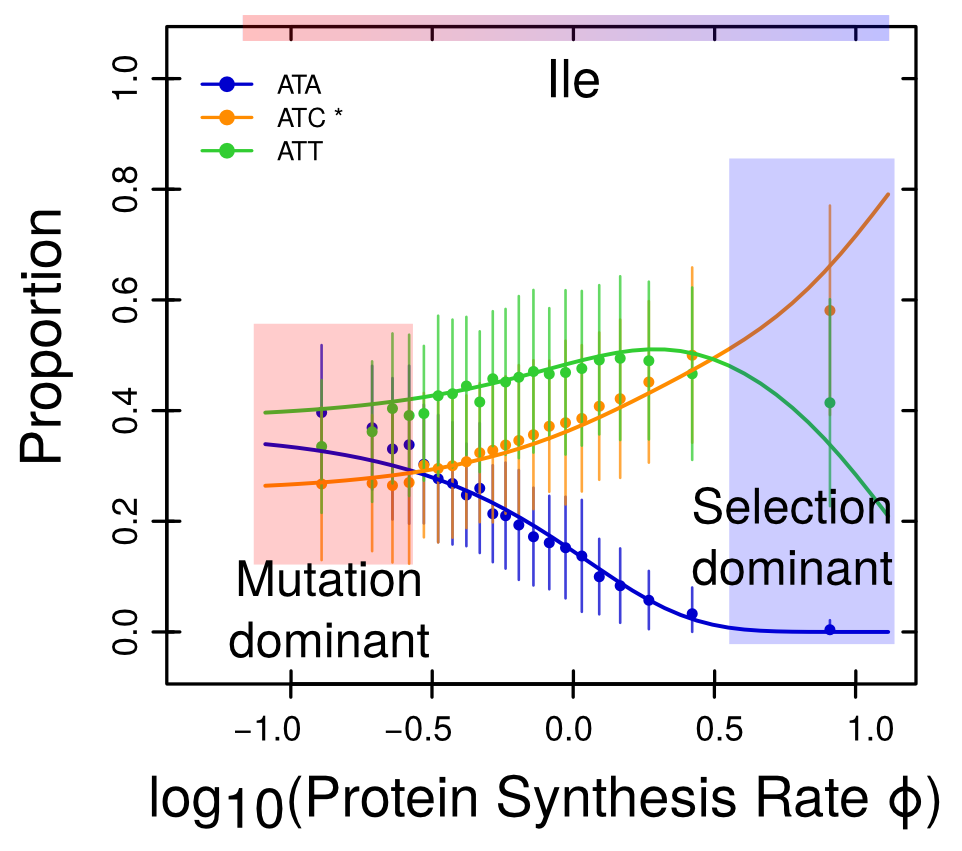
\includegraphics[width=0.6\textwidth]{ch1/expl_model}
	\caption{\ROC model behavior for Isoleucine.
	The proportion of each codon observed changes with protein synthesis rate.
	Mutation is dominant when protein synthesis rate is low, mutationally favored codons are observed with the highest frequency.
	With the increase of protein synthesis rate, the influence of selection increases until the system is dominated by selection.
	The selectively favored codon is observed with the highest frequency.}
	\label{fig:expl_model}
\end{figure}
\doublespacing

For example, strand specific mutation bias \citep{Lafay1999,Romero2000}, differences in the tRNA pool throughout life stages \citep{sagi2016}, or introgressions and horizontal gene transfer \citep{medigue1991,lawrence1997} can produce multiple genomic environments.
Chapter \ref{ch:anacoda} extends the mechanistic model \ROC \cite{gilchrist2015} to allow for a mixture distribution of mutation and selection parameters \cite{landerer2018} and provides researchers with a software tool to address intra genomic variation in codon usage.
However, there is a significant difference to classical mixture approaches.
In addition to gene population specific parameters, \ROC also estimates a gene specific parameter (protein synthesis rate). 
Therefore, the protein synthesis rate for each gene has to be estimated assuming that the a gene is in each gene population.
This can provide additional insight into the adaptiveness of a gene to alternative genomic environments.
Figure \ref{fig:expl_model} illustrates how the proportions of synonymous codons change with increasing protein synthesis rate.
When the protein synthesis rate is low, mutation bias between codons dominates the proportions of synonymous codons while increasing protein synthesis increases the strength of selection (see \cite{gilchrist2015} for details). 

In chapter \ref{ch:kluyveri}, I apply AnaCoDa to analyze the synonymous codon usage of the yeast \kluyveri which experienced a large scale introgression replacing the whole left arm of chromosome C \citep{friedrich2015}.
I studied the differences in the parameters describing codon usage between the endogenous \kluyveri genes and the introgressed exogenous genes.
Recognizing the differences in codon usage between the endogenous and exogenous genes allowed me to improve prediction of protein synthesis rate, and separate the effects of mutation bias and selection in the endogenous \kluyveri genes and the introgressed exogenous genes.
This information was used to determine a potential donor lineage in \gossypii, estimate the time since introgression, and estimate the genetic load of the introgression.

\section{Benefit: Selection on Amino acids}
Genes are evolving with natural selection favoring proteins that encode their function optimally, with mutations and genetic drift reducing functionality.
Amino acid preference and the relative strength of mutation, selection, and genetic drift usually varies between sites along the protein sequence.
The number of parameters required to describe protein fitness increases exponentially with the length of the protein if interactions between sites are accounted for.
Attempts to incorporate selection into phylogenetic approaches are, therefore, limited to site specific selection.
The goal of chapter \ref{ch:phylogeny} is to estimate the strength of site specific selection on amino acids from protein coding sequences in a phylogenetic framework.

\singlespacing
\begin{figure}
     \centering
	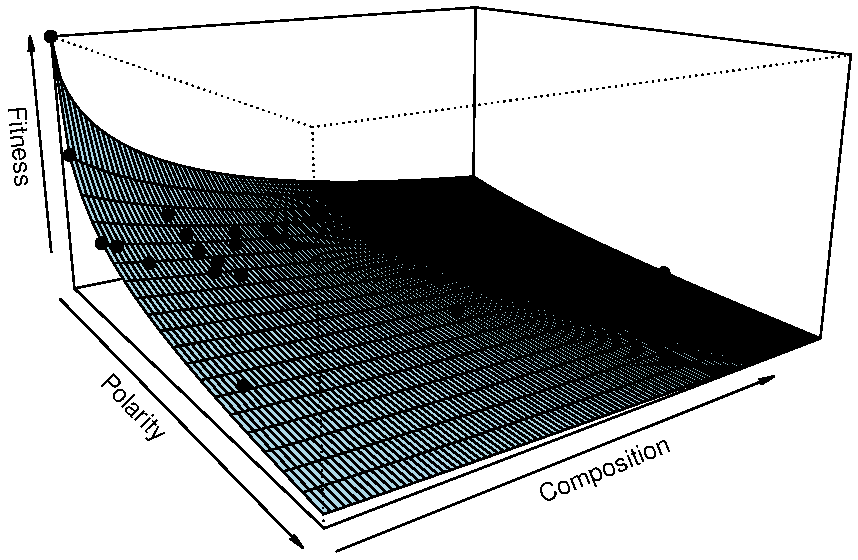
\includegraphics[width=0.7\textwidth]{ch1/decl_fitness2}
	\caption{Decline in fitness with distance in \PC space from the optimal amino acid. 
	Fitness decline of amino acids (black dots) relative to optimal amino acid (Alanine). Weighting of \PC properties according to \citet{grantham1974}.
	The full fitness surface can be described but only 20 discrete amino acid states are available for selection to act on.}
	\label{fig:decl_fit}
\end{figure}
\doublespacing

Ignoring interactions between sites allows to describe the site specific fitness landscape of a protein.
Some approaches rely on the description of the full fitness landscape and therefore require $19 \times L$, where $L$ is the length of the peptide in amino acids, parameters \citep{LartillotAndPhilippe2004,le2008,wang2008,holder2008,wu2013,tamuri2014}.
As this is still a large number of parameters the incorporation of experimentally determined site specific selection on amino acids is an attractive alternative \citep{bloom2014, thyagarajan2014, bloom2017}. 
Alternatively, assumptions about the nature of selection can reduce the number of parameters required.
For example, frequency dependent selection \citep{GoldmanAndYang1994, MuseAndGaut1994, thorne1996} or stabilizing selection \citep{beaulieu2019} allow for a reduction in fitness of amino acids with distance in \PC space.

\selac \citep{beaulieu2019} is a model of stabilizing selection that assesses the fitness of each amino acid relative to the fitness peak (Figure \ref{fig:decl_fit}).
The ftness of an amino acid is assumed to decline exponentially with distance to the optimal amino acid in \PC space.
In chapter \ref{ch:phylogeny} I apply \selac to the $\beta$-lactamase TEM and estimate site specific selection on amino acids and compare the inferred fitness landscape to empirical estimates from deep mutation scanning experiments \citep{stiffler2016}.
I find that experimentally informed amino acid preferences improve model fit but do not accurately reflect the evolution of TEM in the wild.
Furthermore, I show that the information on site specific selection on amino acids can be extracted from protein coding sequences by models rooted in first principles like \selac.





    \chapter{AnaCoDa: Analyzing Codon Data with Bayesian mixture models} 
\label{ch:anacoda}


\clearpage
\pagebreak
This chapter is a lightly revised version of a paper by the same name published in Bioinformatics and co-authored with Alexander Cope, Russell Zaretzki, and Michael A. Gilchrist.\\
\newline
\newline
C. Landerer, A. Cope, R. Zaretzki, M.A. Gilchrist, AnaCoDa: analyzing codon data with Bayesian mixture models, Bioinformatics, 34, 2018, 2496-2498


%%%%%%%%%%%%%%%%%%
%%% %%   ABSTRACT   %%%%%%
%%%%%%%%%%%%%%%%%%
\section{Abstract}
%\begin{center}\textbf{Abstract}\end{center}
%\begin{abstract}
\textbf{\package} is an R package for estimating biologically relevant parameters of mixture models, such as selection against translation inefficiency, nonsense error rate, and ribosome pausing time, from genomic and high throughput datasets.
\package provides an adaptive Bayesian MCMC algorithm, fully implemented in C++ for high performance with an ergonomic R interface to improve usability. 
\package employs a generic object-oriented design to allow users to extend the framework and implement their own models.
Current models implemented in \package can accurately estimate biologically relevant parameters given either protein coding sequences or ribosome foot-printing data.
Optionally, \package can utilize additional data sources, such as gene expression measurements, to aid model fitting and parameter estimation.
By utilizing a hierarchical object structure, some parameters can vary between sets of genes while others can be shared.
Genes may be assigned to clusters or membership may be estimated by \package.
This flexibility allows users to estimate the same model parameter under different biological conditions and categorize genes into different sets based on shared model properties embedded within the data.
\package also allows users to generate simulated data which can be used to aid model development and model analysis as well as evaluate model adequacy.
Finally, \package contains a set of visualization routines and the ability to revisit or re-initiate previous model fitting, providing researchers with a well rounded easy to use framework to analyze genome scale data.

\section*{Availability:}
\textbf{\package} is freely available under the Mozilla Public License 2.0
on CRAN (\url{https://cran.r-project.org/web/packages/AnaCoDa/}).

%\end{abstract}

\newpage

%%%%%%%%%%%%%%%%%%
%%%   INTRODUCTION   %%%%%%
%%%%%%%%%%%%%%%%%%
\section{Introduction}

\package is  an open-source software implemented in R \citep{rcore} that allows researchers to analyze genome-scale data like coding sequences and ribosome footprinting data using evolutionary or analytical models in a Bayesian framework. 
\package was developed to analyze selection on synonymous codon usage in the form of ribosome overhead cost \citep{gilchrist2015,wallace2013,shah2011}.
However, other codon metrics like the codon adaptation index \citep{sharp1987} or the effective number of codons \citep{Wright1990} are also provided as reference.
%% addded to introduction
In addition, three currently unpublished models to analyze coding sequences for evidence of selection against nonsense errors and estimate ribosome pausing times from ribosome footprinting data are included.
\package implements an adaptive Gibbs sampler within a Metropolis-Hastings Monte Carlo Markov Chain (MCMC). 
This allows for the incorporation of prior knowledge such as observed gene expression levels and easy sampling from the posterior distribution to estimate parameter values and quantify degree of uncertainty.
\package provides a mixture distribution option to all implemented models, combining genes into sets by estimating the posterior probabilities of set membership based on gene-set specific parameters shared by all genes assigned to a given set. 
\package provides a generic, mixture distribution option to all implemented models, allowing for the estimation of condition specific parameters or the automatic categorization of data into different sets based on differences in their posterior probabilities of set membership.
In addition to the four models provided, \package provides a modular infrastructure such that additional genome scale or even phylogenetic models can be integrated.

The \package framework works with \package requires gene specific data such as codon frequencies obtained from coding sequences or position specific footprint counts.
Conceptually, \package allows for three different types of parameters.
The first type are gene specific parameters such as protein synthesis rate or relative functionality.
The second type are gene-set specific parameters, such as mutation bias terms or translation error rates.
These parameters are shared across genes within a set and can be exclusive to a single set or shared with other sets.
While the number of gene sets must be pre-defined by the user, set assignment of genes can be pre-defined or estimated as part of the model fitting.
Estimation of the set assignment provides the probability of a gene being assigned to a set allowing the user to asses the uncertainty in each assignment.
The third type are hyperparameters allowing for the construction and analysis of hierarchical model. 
Hyperparameters control the prior distribution for gene and gene-set specific parameters such as mutation bias or protein synthesis rate.

%%%%%%%%%%%%%%%%%%
%%%%%% FEATURES   %%%%%%
%%%%%%%%%%%%%%%%%%
\section{Features}
\package provides an interface written in R, a freely available programming language noted for its ease of use for even inexperienced programmers. 
As a result, \package is accessible to researchers with minimal computational experience. 

The interface of \package is designed for quick and efficient data analysis.
Generally, the only input needed for fitting a model to the data are protein-coding codon sequences in the form of a FASTA file or a flat-file containing codon counts obtained from ribosome foot-printing experiments. 
\package also provides visualization functionality, including plotting functions to compare parameter estimates for different mixture distributions and display codon usage patterns. 
In addition, diagnostic functions such as those for calculating and visualizing the degree of autocorrelation in the parameter traces are provided.

%%%%%%%%%%%%%%%%%%%
\subsubsection{Robust and efficient model fitting}
\package has built-in features designed to improve the robustness and performance of the implemented MCMC approach. 
For example, the implemented MCMC automatically adapts the proposal width for sampled parameters such that an user defined acceptance range is met, improving sampling efficiency of the MCMC and computational performance.
Even though \package is written in C++, analysis of large datasets and/or complex models can be very computationally intensive.
To protect users from computer failures or aid in the collection of additional MCMC samples, \package can periodically produce output checkpoint files, which can be used to restart an MCMC chain from a previous time point.
In addition, \package automatically thins all parameter traces -  meaning only every $k^{th}$ sample is kept - increasing the effective number of samples and reducing its memory footprint. 

Although \package is provided as an R package, the main computational work is implemented in C++.
Because R does not provide native C++ support, Rcpp was employed to expose whole C++ classes as modules to R \citep{rcpp_package}.
Using Rcpp eliminates time consuming data transfers between the R environment and the C++ core during model fitting, resulting in improved computational performance and allows for a fully object-oriented code design \citep{ood_book}. 
As expected, the runtime of \package scales linearly with genome size and number of iterations, and scales polynomially with the number of mixture distributions in the data set. 
The polynomial increase in runtime with the number of mixture distributions is due to the necessity to condition the gene assignment on the estimation of gene specific parameters, such as, protein synthesis rate.

%%%%%%%%%%%%%%%%%%%%%
\subsubsection{Data Simulation}
In addition to fitting the models to datasets, \package can be used to generate simulated data sets as well.
On their own, simulated datasets are useful for model development and analysis.
Simulating data under different conditions allows the user to explore model behavior and explore theoretical scenarios. 
Different conditions can include the addition or elimination of parameters, or simply allowing a set of parameter values to vary.
Fitting models to simulated data can provide insight into potential pitfalls or shortcomings when fitting observational data and can serve as the basis for evaluating model adequacy of a model fit to observational data \citep{gumi2015}.
Significant differences between simulated and observational data suggests the current set of parameters or the model as a whole fail to include or adequately represent biological mechanisms underlying the observed data.
 
%%%%%%%%%%%%%%%%%%%%%
\subsubsection{Available models}
\package currently provides codon models for analyzing genome scale data.
The ROC model implements and extends the codon usage bias (CUB) models developed by \citet{gilchrist2015,wallace2013,shah2011}, which can reliably estimate the strength of selection on \underline{r}ibosome \underline{o}verhead \underline{c}ost, mutation bias and allows for the inference of protein synthesis rates.
This model allows for the separation of effects of mutation and selection based on gene ordering by protein synthesis rate, and the addition of a mixture distribution allows for gene clustering based on mutation bias and selection for translation efficiency.
In addition to identifying the most efficient codons, ROC provides estimates of mutation bias allowing the approximation of mutation ratios between codons \citep{gilchrist2015,wallace2013}.

The ability to estimate protein synthesis rates in the absence of empirical data is useful for investigating CUB of non-model organisms for which such data is lacking and enables the usage of protein synthesis rate in comparative frameworks or other analyses requiring protein synthesis rate information \citep{dunn2018}.
Use of the mixture model allows for the investigation of CUB heterogeneity at the genome or gene level.  
Following the same framework, additional models included in \package provide estimates of codon-specific nonsense errors rates (FONSE) and ribosome pausing times (PA and PANSE).

Parameters estimated with the evolutionary models ROC and FONSE represent evolutionary averages and do not depend on experimental conditions. 
In contrast, PA and PANSE estimate the distribution of biologically relevant parameters like ribosome pausing times along a gene from experimental data such as ribosome footprinting data. 
The distribution can be dependent (PANSE) or independent (PA) of evidence for nonsense errors in the data.  


%%%%%%%%%%%%%%%%%%%%%%%%%%%%%%%%%%%%%%%%%%%%%%%%%%%%
\section{Appendix: Supplementary Material}
AnaCoDa allows for the estimation of biologically relevant parameters like mutation bias or ribosome pausing
time, depending on the model employed. Bayesian estimation of parameters is performed using an adaptive
Metropolis-Hasting within Gibbs sampling approach. Models implemented in AnaCoDa are currently able to
handle gene coding sequences and ribosome footprinting data.

\subsection{The AnaCoDa framework}
The AnaCoDa framework works with gene specific data such as codon frequencies or position specific footprint
counts. Conceptually, AnaCoDa uses three different types of parameters.

\begin{itemize}
	\item The first type of parameters are \textbf{gene specific parameters} such as gene expression level or functionality.
Gene-specific parameters are estimated separately for each gene and can vary between potential gene
categories or sets.
	\item The second type of parameters are \textbf{gene-set specific parameters}, such as mutation bias terms or
translation error rates. These parameters are shared across genes within a set and can be exclusive to a
single set or shared with other sets. While the number of gene sets must be pre-defined by the user, set
assignment of genes can be pre-defined or estimated as part of the model fitting. Estimation of the set
assignment provides the probability of a gene being assigned to a set allowing the user to asses the
uncertainty in each assignment.
	\item The third type of parameters are \textbf{hyperparameters}, such as parameters controlling the prior distribution
for mutation bias or error rate. Hyperparameters can be set specific or shared across multiple sets
and allow for the construction and analysis of hierarchical models, by controlling prior distributions for
gene or gene-set specific parameters.
\end{itemize}

\subsubsection{Analyzing protein coding gene sequences}
AnaCoDa always requires the following four objects:
\begin{itemize}
	\item \textbf{Genome} contains the codon data read from a fasta file as well as empirical protein synthesis rate in
the form of a comma separated (.csv) ID/Value pairs.
	\item \textbf{Parameter} represents the parameter set (including parameter traces) for a given genome. The
parameter object also hold the mapping of parameters to specified sets.
	\item \textbf{Model} allows you to specify which model should be applied to the genome and the parameter object.
	\item \textbf{MCMC} specifies how many samples from the posterior distribution of the specified model should be
stored to obtain parameter estimates.
\end{itemize}

\subsection{AnaCoDa setup}
\subsubsection{Application of codon model to single genome}
In this example we are assuming a genome with only one set of gene-set specific parameters, hence \textbf{num.mixtures $ = 1$}. 
We assign all genes the same gene-set, and provide an initial value for the hyperparameter sphi ($s_\phi$). $s_\phi$ controls the lognormal prior distribution on the gene specific parameters like the protein synthesis rate $\phi$. 
To ensure identifiability the expected value of the prior distribution is assumed to be $1$.

\begin{equation}
E[\phi] = \exp\left(m_\phi + \frac{s^2_\phi}{2}\right) = 1
\end{equation}
Therefore the mean $m_\phi$ is set to be $-\frac{s^2_\phi}{2}$.
For more details see \citet{gilchrist2015}.

After choosing the model and specifying the necessary arguments for the MCMC routine, the MCMC is run

\begin{lstlisting}[language=R]
genome <- initializeGenomeObject(file = "genome.fasta")
parameter <- initializeParameterObject(genome = genome, sphi = 1, 
			num.mixtures = 1, 
			gene.assignment = rep(1, length(genome)))
model <- initializeModelObject(parameter = parameter, model = "ROC")
mcmc <- initializeMCMCObject(samples = 5000, thinning = 10, 
			adaptive.width=50)
runMCMC(mcmc = mcmc, genome = genome, model = model)
\end{lstlisting}

\textbf{runMCMC} does not return a value, the results of the MCMC are stored automatically in the mcmc and parameter
objects created earlier.

\begin{quote}
\textbf{Please note that AnaCoDa utilizes C++ object orientation and therefore employs pointer structures. 
This means that no return value is necessary for such objects as they are modified within the the runMCMC routine. 
You will find that after a completed run, the parameter object will contain all necessary information without being directly passed into the MCMC routine. 
This might be confusing at first as it is not default R behavior.}
\end{quote}

\subsubsection{Application of codon model to a mixture of genomes}
This case applies if we assume that parts of the genome differ in their gene-set specific parameters. 
This could be due to introgression events or strand specific mutation difference, horizontal gene transfers or other reasons. 
We make the assumption that all sets of genes are independent of one another. 
For two sets of gene-set specific parameter with a random gene assignment we can use:

\begin{lstlisting}[language=R]
parameter <- initializeParameterObject(genome = genome, 
			sphi = c(0.5, 2), num.mixtures = 2,
			gene.assignment = sample.int(2, 
				length(genome), replace = T))
gene.assignment = sample.int(2, length(genome), replace = T))
\end{lstlisting}

To accommodate for this mixing we only have to adjust \textbf{sphi}, which is now a vector of length 2, \textbf{num.mixtures},
and \textbf{gene.assignment}, which is chosen at random here.

\subsubsection{Empirical protein synthesis rate values}
To use empirical values as prior information one can simply specify an observed.expression.file when
initializing the genome object.

\begin{lstlisting}[language=R]
genome <- initializeGenomeObject(file = "genome.fasta",
		observed.expression.file = "synthesis_values.csv")
\end{lstlisting}

These observed expression or synthesis values ($\Phi$) are independent of the number of gene-sets. 
The error in the observed $\Phi$ values is estimated and described by sepsilon ($s_\epsilon$). 
The csv file can contain multiple observation sets separated by comma.
For each set of observations an initial $s_\epsilon$ has to be specified.

\begin{lstlisting}[language=R]
# One case of observed data
sepsilon <- 0.1
# Two cases of observed data
sepsilon <- c(0.1, 0.5)
# ...
# Five cases of observed data
sepsilon <- c(0.1, 0.5, 1, 0.8, 3)
parameter <- initializeParameterObject(genome = genome, sphi = 1, 
			num.mixtures = 1,
			gene.assignment = rep(1, length(genome)),
			init.sepsilon = sepsilon)
\end{lstlisting}

In addition one can choose to keep the noise in the observations ($s_\epsilon$) constant by using the \textbf{fix.observation.noise} flag in the model object.

\begin{lstlisting}[language=R]
model <- initializeModelObject(parameter = parameter, model = "ROC",
fix.observation.noise = TRUE)
\end{lstlisting}

\subsubsection{Fixing parameter types}
It can sometime be advantages to fix certain parameters, like the gene specific parameters. 
For example in cases where only few sequences are available but gene expression measurements are at hand we can fix the gene specific parameters to increase confidence in our estimates of gene-set specific parameters.

We again initialize the \textbf{genome}, \textbf{parameter}, and \textbf{model} objects.

\begin{lstlisting}[language=R]
genome <- initializeGenomeObject(file = "genome.fasta")
parameter <- initializeParameterObject(genome = genome, sphi = 1, 
			num.mixtures = 1,
			gene.assignment = rep(1, length(genome)))
model <- initializeModelObject(parameter = parameter, model = "ROC")
\end{lstlisting}

To fix gene specific parameters we will set the \textbf{est.expression} flag to \textbf{FALSE}. This will estimate only gene-set
specific parameters, hyperparameters, and the assignments of genes to various sets.

\begin{lstlisting}[language=R]
mcmc <- initializeMCMCObject(samples, thinning=1, 
			adaptive.width=100, est.expression=FALSE, 
			est.csp=TRUE, est.hyper=TRUE, est.mix=TRUE)
\end{lstlisting}

If we would like to fix gene-set specific parameters we instead disable the \textbf{est.csp} flag.

\begin{lstlisting}[language=R]
mcmc <- initializeMCMCObject(samples, thinning=1, 
			adaptive.width=100, est.expression=TRUE, 
			est.csp=FALSE, est.hyper=TRUE, est.mix=TRUE)
\end{lstlisting}

The same applies to the hyper parameters (\textbf{est.hyper}),

\begin{lstlisting}[language=R]
mcmc <- initializeMCMCObject(samples, thinning=1, 
			adaptive.width=100, est.expression=TRUE, 
			est.csp=TRUE, est.hyper=FALSE, est.mix=TRUE)
\end{lstlisting}

and gene set assignment (\textbf{est.mix}).

\begin{lstlisting}[language=R]
mcmc <- initializeMCMCObject(samples, thinning=1, 
			adaptive.width=100, est.expression=TRUE, 
			est.csp=TRUE, est.hyper=TRUE, est.mix=FALSE)
\end{lstlisting}

We can use these flags to fix parameters in any combination.

\subsubsection{Combining various gene-set specific parameters to a gene-set description.}

We distinguish between three simple cases of gene-set descriptions, and the ability to customize the parameter
mapping. The specification is done when initializing the parameter object with the \textbf{mixture.definition}
argument.

We encounter the simplest case when we assume that all gene sets are independent.

\begin{lstlisting}[language=R]
parameter <- initializeParameterObject(genome = genome, 
			sphi = c(0.5, 2), num.mixtures = 2,
			gene.assignment = sample.int(2, 
				length(genome), replace = T),
			mixture.definition = "allUnique")
\end{lstlisting}

The \textbf{allUnique} keyword allows each type of gene-set specific parameter to be estimated independent of parameters describing other gene sets.

In case we want to share mutation parameter between gene sets we can use the keyword \textbf{mutationShared}

\begin{lstlisting}[language=R]
parameter <- initializeParameterObject(genome = genome, 
			sphi = c(0.5, 2), num.mixtures = 2,
			gene.assignment = sample.int(2, 
				length(genome), replace = T),
			mixture.definition = "mutationShared")
\end{lstlisting}

This will force all gene sets to share the same mutation parameters.

The same can be done with parameters describing selection, using the keyword \textbf{selectionShared}

\begin{lstlisting}[language=R]
parameter <- initializeParameterObject(genome = genome, 
			sphi = c(0.5, 2), num.mixtures = 2,
			gene.assignment = sample.int(2, 
				length(genome), replace = T),
			mixture.definition = "selectionShared")
\end{lstlisting}

For more intricate compositions of gene sets, one can specify a custom $n \times 2$ matrix, where $n$ is the number of gene sets, to describe how gene-set specific parameters should be shared. 
Instead of using the \textbf{mixture.definition} argument one uses the \textbf{mixture.definition.matrix} argument.

The matrix representation of \textbf{mutationShared} can be obtained by

\begin{lstlisting}[language=R]
# [,1] [,2]
#[1,] 1 1
#[2,] 1 2
#[3,] 1 3
def.matrix <- matrix(c(1,1,1,1,2,3), ncol=2)
parameter <- initializeParameterObject(genome = genome, 
			sphi = c(0.5, 2, 1), num.mixtures = 3,
			gene.assignment = sample.int(3, 
				length(genome), replace = T),
			mixture.definition.matrix = def.matrix)
\end{lstlisting}

Columns represent mutation and selection, while each row represents a gene set. 
In this case we have three gene sets, each sharing the same mutation category and three different selection categories.
In the same way one can produce the matrix for three independent gene sets equivalent to the \textbf{allUnique} keyword.

\begin{lstlisting}[language=R]
# [,1] [,2]
#[1,] 1 1
#[2,] 2 2
#[3,] 3 3
def.matrix <- matrix(c(1,2,3,1,2,3), ncol=2)
\end{lstlisting}

We can also use this matrix to produce more complex gene set compositions.

\begin{lstlisting}[language=R]
# [,1] [,2]
#[1,] 1 1
#[2,] 2 1
#[3,] 1 2
def.matrix <- matrix(c(1,2,1,1,1,2), ncol=2)
\end{lstlisting}

In this case gene set one and three share their mutation parameters, while gene set one and two share their selection parameters.

\subsubsection{Checkpointing}

AnaCoDa does provide checkpointing functionality in case runtime has to be restricted. 
To enable checkpointing, one can use the function \textbf{setRestartSettings}.

\begin{lstlisting}[language=R]
# writing a restart file every 1000 samples
setRestartSettings(mcmc, "restart_file", 1000, write.multiple=TRUE)
# writing a restart file every 1000 samples 
# but overwriting it every time
setRestartSettings(mcmc, "restart_file", 1000, write.multiple=FALSE)
\end{lstlisting}

To re-initialize a parameter object from a restart file one can simply pass the restart file to the initialization function:

\begin{lstlisting}[language=R]
initializeParameterObject(init.with.restart.file="restart_file.rst")
\end{lstlisting}

\subsubsection{Load and save parameter objects}
AnaCoDa is based on C++ objects using the Rcpp \citep{rcpp_package}. 
This comes with the problem that C++ objects are by default not serializable and can therefore not be saved/loaded with the default R save/load functions.

AnaCoDa however, does provide functions to load and save parameter and mcmc objects. 
These are the only two objects that store information during a run.

\begin{lstlisting}[language=R]
#save objects after a run
runMCMC(mcmc = mcmc, genome = genome, model = model)
writeParameterObject(parameter = parameter, file = "parameter.Rda")
writeMCMCObject(mcmc = mcmc, file = "mcmc_out.Rda")
\end{lstlisting}

As \textbf{genome}, and \textbf{model} objects are purely storage containers, no save/load function is provided at this point, but will be added in the future.

\begin{lstlisting}[language=R]
#load objects
parameter <- loadParameterObject(file = "parameter.Rda")
mcmc <- loadMCMCObject(file = "mcmc_out.Rda")
\end{lstlisting}

\subsection{File formats}

\subsubsection{protein coding sequence}
Protein coding sequences are provided by fasta file with the default format. One line containing the sequence
id starting with $>$ followed by the id and one or more lines containing the sequence. The sequences are
expected to have a length that is a multiple of three. If a codon can not be recognized (e.g AGN) it is ignored.

\begin{verbatim}
>YAL001C
TTGGTTCTGACTCATTAGCCAGACGAACTGGTTCAA
CATGTTTCTGACATTCATTCTAACATTGGCATTCAT
ACTCTGAACCAACTGTAAGACCATTCTGGCATTTAG
>YAL002W
TTGGAACAAAACGGCCTGGACCACGACTCACGCTCT
TCACATGACACTACTCATAACGACACTCAAATTACT
TTCCTGGAATTCCGCTCTTAGACTCAACTGTCAGAA
\end{verbatim}

\subsubsection{Empirical gene expression}

Empirical expression or gene specific parameters are provided in a csv file format. The first line is expected to
be a header describing each column. The first column is expected be the gene id, and every additional column
is expected to be represent a measurement. Each row corresponds to one gene and contains all measurements
for that gene, including missing values.

\begin{verbatim}
>YAL001C
ORF,DATA_1,DATA_2,...DATA_N
YAL001C,0.254,0.489,...,0.156
YAL002W,1.856,1.357,...,2.014
YAL003W,10.45,NA,...,9.564
YAL005C,0.556,0.957,...,0.758
\end{verbatim}

\subsubsection{Ribosome foot-printing counts}

Ribosome foot-printing (RFP) counts are provided in a csv file format. The first line is expected to be a
header describing each column. The columns are expected in the following order gene id, position, codon,
rfpcount. Each row corresponds to a single codon with an associated number of ribosome footprints.

\begin{verbatim}
GeneID,Position,Codon,rfpCount
YBR177C, 0, ATA, 8
YBR177C, 1, CGG, 1
YBR177C, 2, GTT, 8
YBR177C, 3, CGC, 1
\end{verbatim}

\subsection{Analyzing and Visualizating results}

\subsubsection{Parameter estimates}

After we have completed the model fitting, we are interested in the results. 
AnaCoDa provides functions to obtain the posterior estimate for each parameter. 
For gene-set specific parameters or codon specific parameters we can use the function \textbf{getCSPEstimates}. 
Again we can specify for which mixture we would like the posterior estimate and how many samples should be used. 
\textbf{getCSPEstimates} has an optional argument filename which will cause the routine to write the result as a csv file instead of returning a \textbf{data.frame}.

\begin{lstlisting}[language=R]
csp_mat <- getCSPEstimates(parameter = parameter, CSP="Mutation", 
			mixture = 1, samples = 1000)
head(csp_mat)
# AA Codon Posterior 0.025% 0.975%
#1 A GCA -0.2435340 -0.2720696 -0.2165220
#2 A GCC 0.4235546 0.4049132 0.4420680
#3 A GCG 0.7004484 0.6648690 0.7351707
#4 C TGC 0.2016298 0.1679025 0.2387024
#5 D GAC 0.5775052 0.5618199 0.5936979
#6 E GAA -0.4524295 -0.4688044 -0.4356677
getCSPEstimates(parameter = parameter, filename = "mutation.csv",
			CSP="Mutation", mixture = 1, samples = 1000)
\end{lstlisting}

To obtain posterior estimates for the gene specific parameters, we can use the function \textbf{getExpressionEstimatesForMixture}.
In the case below we ask to get the gene specific parameters for all genes, and under the assumption each gene is assigned to mixture $1$.

\begin{lstlisting}[language=R]
phi_mat <- getExpressionEstimates(parameter = parameter,
			gene.index = 1:length(genome),
			samples = 1000)
head(phi_mat)
# PHI log10.PHI Std.Error log10.Std.Error 0.025 0.975 log10.025 ...
#[1,] 0.2729446 -0.6188447 0.0001261525 2.362358e-04 0.07331819 ...
#[2,] 1.4221716 0.1498953 0.0001669425 5.194123e-05 1.09593642 ...
#[3,] 0.7459888 -0.1512764 0.0002313539 1.529267e-04 0.31559618 ...
#[4,] 0.6573082 -0.2030291 0.0001935466 1.400333e-04 0.31591233 ...
#[5,] 1.6316901 0.2098120 0.0001846631 4.986347e-05 1.28410352 ...
#[6,] 0.6179711 -0.2286806 0.0001744928 1.374863e-04 0.28478950 ...
\end{lstlisting}

However we can decide to only obtain certain gene parameters. in the first case we sample 100 random genes.

\begin{lstlisting}[language=R]
# sampling 100 genes at random
phi_mat <- getExpressionEstimates(parameter = parameter,
			gene.index = sample(1:length(genome), 100),
			samples = 1000)
\end{lstlisting}

Furthermore, AnaCoDa allows to calculate the selection coefficient s for each codon and each gene. We can
use the function \textbf{getSelectionCoefficients} to do so. Please note, that this function returns the $\log(sNe)$.

\textbf{getSelectionCoefficients} returns a matrix with $\log(sNe)$ relative to the most efficient synonymous codon.

\begin{lstlisting}[language=R]
selection.coefficients <- getSelectionCoefficients(genome = genome,
			parameter = parameter, samples = 1000)
head(selection.coefficients)
# GCA GCC GCG GCT TGC TGT GAC GAT ...
#SAKL0A00132g -0.1630284 -0.008695144 -0.2097771 0 -0.1014373 ...
#SAKL0A00154g -0.8494558 -0.045305847 -1.0930388 0 -0.5285367 ...
#SAKL0A00176g -0.4455753 -0.023764823 -0.5733448 0 -0.2772397 ...
#SAKL0A00198g -0.3926068 -0.020939740 -0.5051875 0 -0.2442824 ...
#SAKL0A00220g -0.9746002 -0.051980440 -1.2540685 0 -0.6064022 ...
#SAKL0A00242g -0.3691110 -0.019686586 -0.4749542 0 -0.2296631 ...
\end{lstlisting}

We can compare these values to the weights from the codon adaptation index (CAI) citep{Sharp1987} or
effective number of codons ($N_c$) \citep{Wright1990} by using the functions \textbf{getCAIweights} and \textbf{getNcAA}.

\begin{lstlisting}[language=R]
cai.weights <- getCAIweights(referenceGenome = genome)
head(cai.weights)
# GCA GCC GCG GCT TGC TGT
#0.7251276 0.6282192 0.2497737 1.0000000 0.6222628 1.0000000
nc.per.aa <- getNcAA(genome = genome)
head(nc.per.aa)
# A C D E F G ...
#SAKL0A00132g 3.611111 1.000000 2.200000 2.142857 1.792453 ...
#SAKL0A00154g 1.843866 2.500000 2.035782 1.942505 1.986595 ...
#SAKL0A00176g 5.142857 NA 1.857143 1.652174 1.551724 3.122449 ...
#SAKL0A00198g 3.800000 NA 1.924779 1.913043 2.129032 4.136364 ...
#SAKL0A00220g 3.198529 1.666667 1.741573 1.756757 2.000000 ...
#SAKL0A00242g 4.500000 NA 2.095890 2.000000 1.408163 3.734043 ...
\end{lstlisting}

We can also compare the distribution of selection coefficients to the CAI values estimated from a reference set of
genes.

\begin{lstlisting}[language=R]
selection.coefficients <- getSelectionCoefficients(genome = genome,
			parameter = parameter, samples = 1000)
s <- exp(selection.coefficients)
cai.weights <- getCAIweights(referenceGenome = ref.genome)
codon.names <- colnames(s)
h <- hist(s[, 1], plot = F)
plot(NULL, NULL, axes = F, xlim = c(0,1), 
			ylim = range(c(0,h$counts)),
			xlab = "s", ylab = "Frequency", 
			main = codon.names[1], cex.lab = 1.2)
lines(x = h$breaks, y = c(0,h$counts), type = "S", lwd=2)
abline(v = cai.weights[1], lwd=2, lty=2)
axis(1, lwd = 3, cex.axis = 1.2)
axis(2, lwd = 3, cex.axis = 1.2)
\end{lstlisting}

\begin{figure}[h]
  \centering
  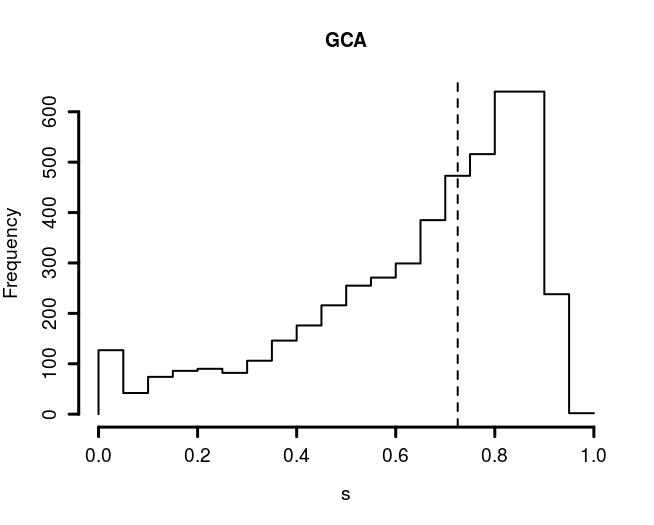
\includegraphics[width=.6\textwidth]{ch2/sel_cai_comp.png}\\
  \caption{Distribution of s for codon GCA for amino acid alanine. Dashed line indicates the CAI weight for
GCA. The comparison provides a more nuanced picture as we can see that the selection on GCA varies
across the genome.}
  \label{fig:sne_dummy}
\end{figure} 

\subsubsection{Diagnostic Plots}
A first step after every run should be to determine if the sampling routine has converged. 
To do that, AnaCoDa provides plotting routines to visualize all sampled parameter traces from which the posterior sample is obtained.
First we have to obtain the \textbf{trace} object stored within our \textbf{parameter} object. 
Now we can simply plot the \textbf{trace} object. The argument \textbf{what} specifies which type of parameter should be plotted.
Here we plot the selection parameter $\Delta \eta$ of the ROC model. 
These parameters are mixture specific and one can decide which mixture set to visualize using the argument \textbf{mixture}.

\begin{lstlisting}[language=R]
trace <- getTrace(parameter)
plot(x = trace, what = "Mutation", mixture = 1)
\end{lstlisting}

\begin{figure}[h]
  \centering
  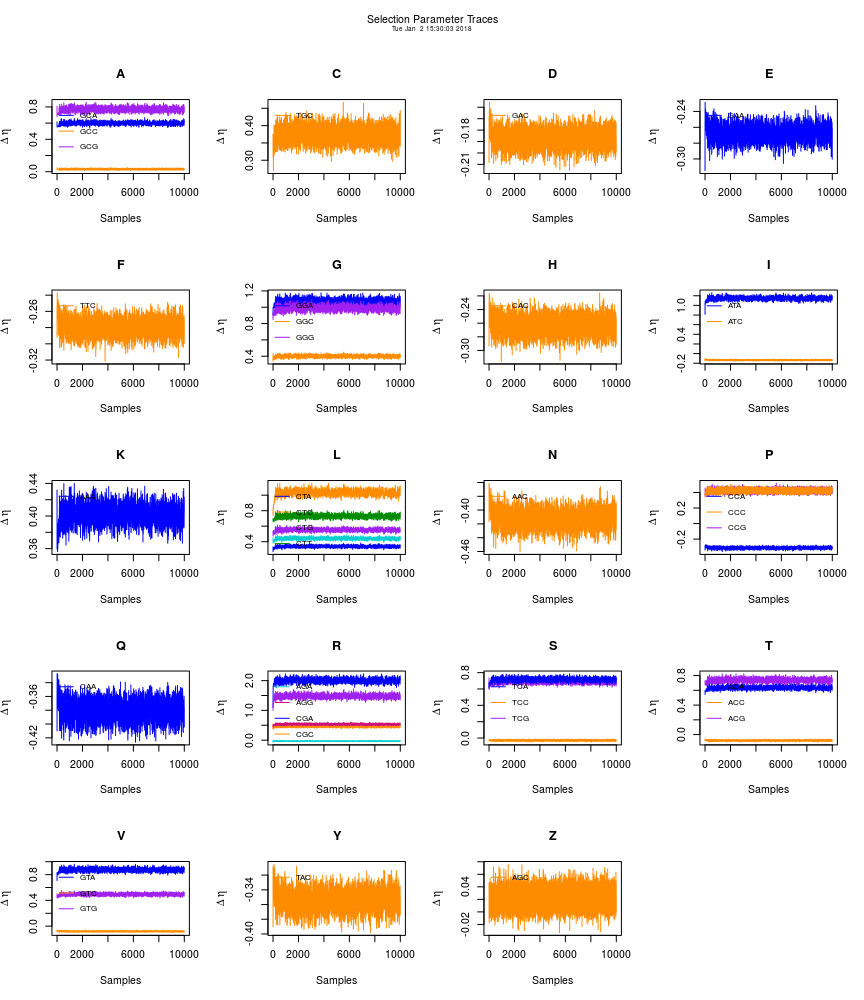
\includegraphics[width=\textwidth]{ch2/selection_trace.png}\\
  \caption{Trace plot showing the traces of all 40 codon specific selection parameters $\Delta \eta$ organized by amino acid.}
  \label{fig:mutation_trace}
\end{figure} 

A special case is the plotting of traces of the protein synthesis rate $\phi$. 
As the number of traces for the different $\phi$ traces is usually in the thousands, a \textbf{geneIndex} has to be passed to determine for which gene the trace should be plotted. 
This allows to inspect the trace of every gene under every mixture assignment.

\begin{lstlisting}[language=R]
trace <- parameter$getTraceObject()
plot(x = trace, what = "Expression", mixture = 1, geneIndex = 669)
\end{lstlisting}

\begin{figure}[h]
  \centering
  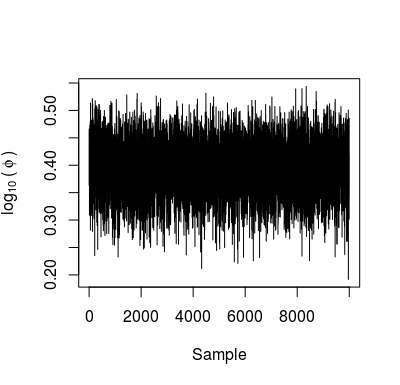
\includegraphics[width=3in]{ch2/expression_trace.png}\\
  \caption{Trace plot showing the protein synthesis trace $\phi$ for gene 669.}
  \label{fig:logphi_trace}
\end{figure} 

We can find the likelihood and posterior trace of the model fit in the \textbf{mcmc object}. 
The trace can be plotted by just passing the \textbf{mcmc} object to the \textbf{plot} routine. 
Again we can switch between $\log(likelihood)$ and $\log(posterior)$ using the argument \textbf{what}. 
The argument \textbf{zoom.window} is used to inspect a specified window in more detail. 
It defaults to the last 10 \% of the trace. 
The $\log(posterior)$ displayed in the figure title is estimated over the \textbf{zoom.window}.

\begin{lstlisting}[language=R]
plot(mcmc, what = "LogPosterior", zoom.window = c(9000, 10000))
\end{lstlisting}


\begin{figure}[h]
  \centering
  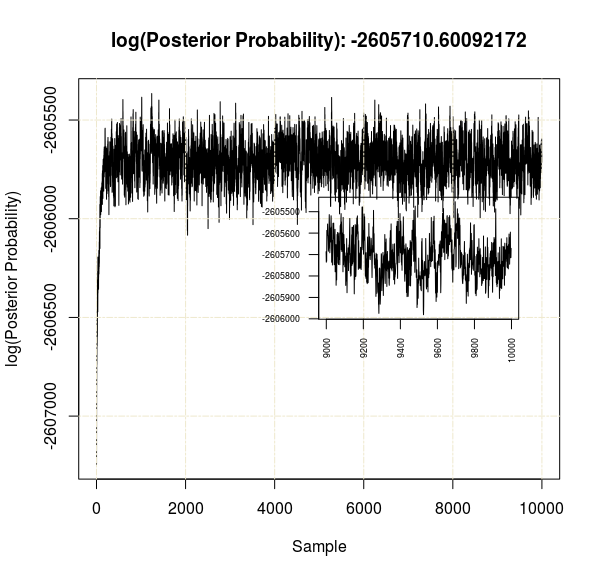
\includegraphics[width=3in]{ch2/logpost_trace.png}\\
  \caption{Trace plot showing the $\log(Posterior)$ trace for the current model fit. Window inset shows the last 1.000 samples}
  \label{fig:logpost_trace}
\end{figure} 

\subsubsection{Model visualization}
We can visualize the results of the model fit by plotting the \textbf{model} object. 
For this we require the model and the \textbf{genome} object. 
We can adjust which mixture set we would like to visualize and how many samples should be used to obtain the posterior estimate for each parameter. 
For more details see \citet{gilchrist2015}.

\begin{lstlisting}[language=R]
# use the last 500 samples from mixture 1 for posterior estimate.
plot(x = model, genome = genome, samples = 500, mixture = 1)
\end{lstlisting}

\begin{figure}[h]
  \centering
  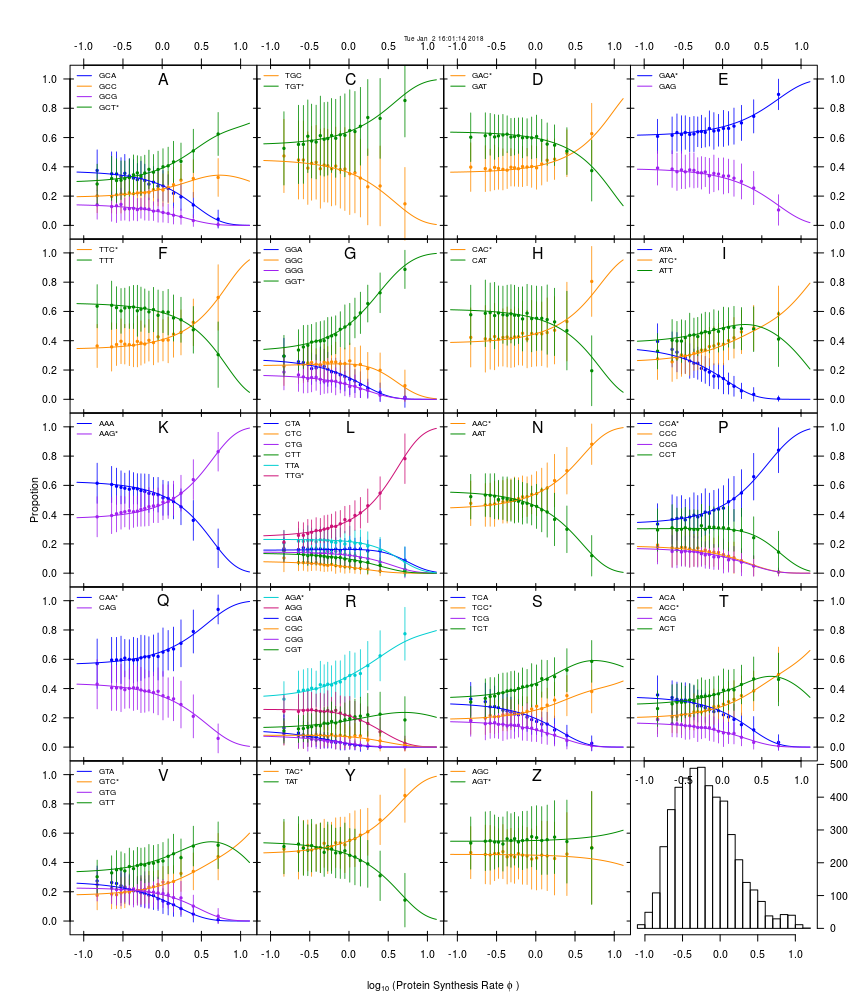
\includegraphics[width=\textwidth]{ch2/model_fit.png}\\
  \caption{Fit of the ROC model for a random yeast. The solid line represent the model fit from the data,
showing how synonymous codon frequencies change with gene expression. The points are the observed mean
frequencies of a codon in that synthesis rate bin and the whisks indicate the standard deviation within the bin.
The codon favored by selection is indicated by a "*". The bottom right panel shows how many genes are
contained in each bin}
  \label{fig:cub_dummy}
\end{figure} 

As AnaCoDa is designed with the idea to allow gene-sets to have independent gene-set specific parameters, AnaCoDa also provides the option to compare different gene-sets by plotting the parameter object. 
Here we compare the selection parameter estimated by ROC for seven yeast species.

\begin{lstlisting}[language=R]
# use the last 500 samples from mixture 1 for posterior estimate.
plot(parameter, what = "Selection", samples = 500)
\end{lstlisting}



\begin{figure}[h]
  \centering
  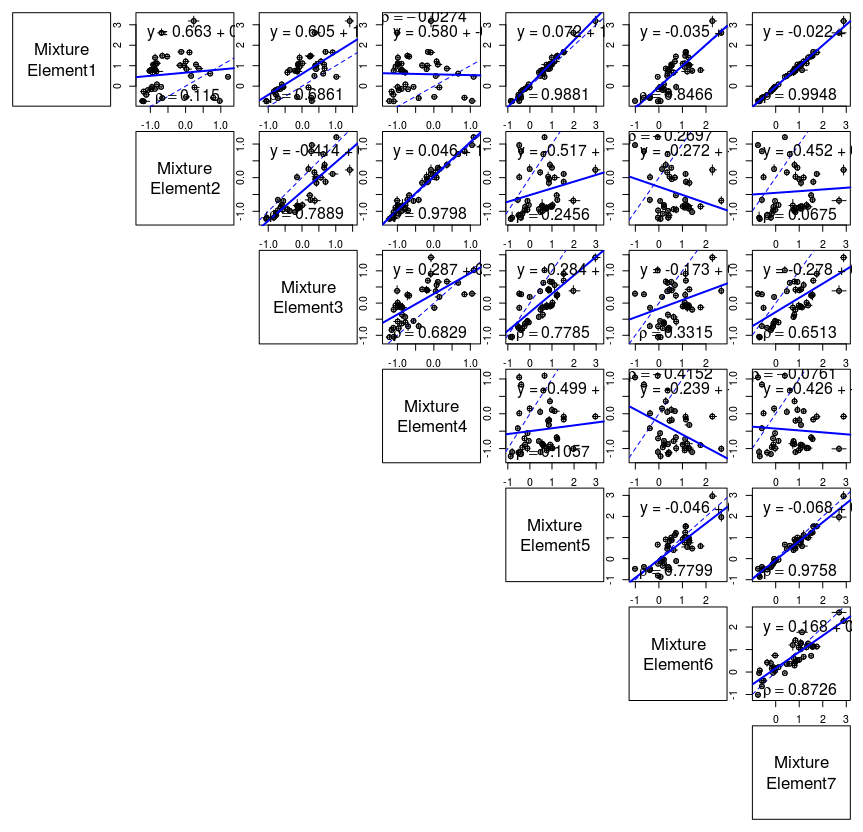
\includegraphics[width=\textwidth]{ch2/param_comp.png}\\
  \caption{Comparison of the selection parameter of seven yeast species estimated with ROC-SEMPPR.}
  \label{fig:comp_dummy}
\end{figure} 
    \chapter{Decomposing mutation and selection to identify mismatched codon usage}
\label{ch:kluyveri}


This chapter is a lightly revised version of a paper to be submitted to Genome Biology and Evolution and co-authored with Michael A. Gilchrist.\\
\newline
\newline
C. Landerer, M.A. Gilchrist, Decomposing mutation and selection to identify mismatched codon usage

\clearpage
\pagebreak

\begin{center}\textbf{Abstract}\end{center}
Codon usage has been used as a measure for adaptation of genes to their cellular environment for decades. 
The introgression of genes from one cellular environment to another may cause well adapted genes to suddenly be less adapted due to them having evolved in a different environment.
As a result, we expect that transferred genes result in a large fitness burden for the new host organism.
Here we examine the yeast \textit{Lachancea kluyveri} which has experienced a large introgression, replacing the left arm of chromosome C ($\sim 10 \%$ of its genome).
The \kluyveri genome provides an opportunity to study the evolution of introgressed genes to a novel cellular environment and estimate the fitness cost such a transfer imposes.
We quantified the effects of mutation bias and selection against translation inefficiency on the codon usage pattern of the endogenous and introgressed exogenous genes using a Bayesian mixture framework.
We found substantial differences in codon usage between the endogenous and exogenous genes, and show that these differences can be largely attributed to a shift in mutation bias from A/T ending codons in the endogenous genes to C/G ending codons in the exogenous genes.
Recognizing the two different signatures of mutation and selection bias improved our ability to predict protein synthesis rate by $17 \%$ and allowed us to accurately assess codon preferences.
In addition we utilize the estimates of mutation bias and selection against translation inefficiency to determine \textit{Eremothecium gossypii} as potential source lineage, estimate the time since introgression to be on the order of $6\times 10^8$ and assess the fitness burden across introgressed loci, showing the advantage of mechanistic models when analyzing codon data.

\newpage


\section{Introduction}

Mutation, selection and genetic drift can be used to quantify the environment a genome has evolved in.
Mutation bias is purely determined by the cellular environment, while the strength and efficacy of selection relative to drift is determined by the cellular environment, e.g. tRNA abundance, and the natural environment e.g. gene expression.
A lineages effective population size determines the efficacy of selection relative to drift.
Synonymous codon usage, the non-uniform usage of codons encoding the same amino acid, is a reflection of both, the cellular and the natural environment.
Decomposing codon usage, therefore, provides us the necessary information to describe the environment a genome has evolved in in terms of its codon usage. 

In general, the strength of selection on codon usage increases with gene expression \citep{ikemura1985, gouy1982}.
Conversely, the impact of mutation bias on codon usage declines with gene expression.
Thus, we can easily imagine that with increasing gene expression, codon usage shifts from a process dominated mutation to a process dominated by selection.
Together, the mutation process favoring specific synonymous codons - or mutation bias -  and the selection for translation efficiency scaled by gene expression and effective population size - or selection bias -  shape codon usage in a genome.
This mutation-selection-drift balance model allows us to explicitly describe the environment in which genes evolve with respect to mutation and selection bias.
Here we show that estimating the influence of mutation bias and selection bias on a gene's codon usage allows us to not only predict protein synthesis rate $\phi$, but also, to infer its history and make predictions about its future with respect to these forces.

Most studies implicitly assume that synonymous codon usage of a genome is shaped by a single cellular environment. 
However, it is easy to think about the influence of multiple cellular environments within a cell, as genes are horizontally transferred, introgress, or as species hybridize.
Genes introduced via horizontal gene transfer, introgression, or hybridization may carry the signature of a different, foreign cellular environment.
These transferred genes may be less adapted to their new cellular environment, potentially imposing large fitness burdens to the organism.
We expect a greater fitness burden of transferred genes if donor and recipient environment differ greatly in their selection bias, making such transfers less likely.
More practically, if transferred genes are unaccounted for, they may distort parameters by biasing estimates.
This can lead to the conclusion of the wrong codon preference for an amino acid when analyzing a genome that has experienced such transfer events.  

In this study, we analyze the synonymous codon usage of the genome of \textit{Lachancea kluyveri}, the earliest diverging lineage of the Lachancea clade.
The Lachancea clade diverged from the Saccharomyces clade prior to the whole genome duplication, about 100 Mya ago.
Since its divergence from the other Lachancea, \kluyveri  has experienced a large introgression of exogenous genes.
The introgression replaced the left arm of the C chromosome and displays a $13 \%$ higher \GC than the endogenous \kluyveri genome \citep{payen2009, friedrich2015}.
These characteristics make \kluyveri an ideal model to study the effects of an introgressed cellular environment and the resulting mismatch codon usage.

Using \ROC, a population genetics Bayesian model, allows us to quantify the cellular environment in which genes have evolved by separating and estimating effects of mutation bias and selection bias, and predicting protein production rate \citep{gilchrist2015}.
We use \ROC to describe two cellular environments reflected in the \kluyveri genome, a native endogenous and an introgressed exogenous environment.
Our results indicate that the difference in \GC between endogenous and exogenous genes mostly to differences in mutation bias.
Recognizing the differences in codon usage between the endogenous and exogenous gene sets also improves our ability to predict protein synthesis rate from the sequence data alone.

With our improved model fits, we obtained more reliable estimates of mutation bias, selection bias and protein synthesis rate, allowing us to address more refined questions of biological importance.
First we determine a potential source lineage of the exogenous genes using a combination of information in codon usage and gene synteny.
We compared estimates of mutation bias (\DM) and selection bias (\DE) for the exogenous genes to 38 yeast lineages and further investigated candidate lineages using synteny.
Second, we estimate the time since introgression and the persistence of the signal of the exogenous cellular environment from our estimates of \DM using an exponential model of decay.
Third, we estimate the selective cost of the mismatched codon usage for the introgression, using our estimates of \DE and protein synthesis rate $\phi$. 
Thus, in addition to being able to estimate codon preference and gene expression to describe codon usage patterns, we also gain insights into the evolution of genes that have been transferred between lineages.

\section{Results}
Model selection and validation confirmed that the \kluyveri genome contains signatures of at least two cellular environments.
We compared model fits of \ROC to the homogeneous \kluyveri genome and the separated sets of endogenous and exogenous genes of 4864 and 497 genes respectively, using AnaCoDa \citep{landerer2018}.
We compared estimates of the cellular environment to describe differences in endogenous and exogenous codon usage.
Furthermore, we utilize the differences in model fit and parameters estimated from the endogenous and exogenous genes to explore the evolution of the exogenous gene set.

AIC indicates that parameter estimates for mutation bias (\DM) and selection bias (\DE) differ greatly between exogenous and endogenous gene sets.
As a result, the partitioning of the \kluyveri genome into an endogenous and exogenous gene set is clearly favored by model selection.
The inclusion of 81 additional parameters ($40$ for \DM, $40$ for \DE, and one for $s_{\phi}$) necessary to describe both gene sets separately improves our model fit by $\sim 75,000$ AIC units (5,311,060 for the combined gene set vs 5,235,598 for the separated gene sets).

\begin{figure}[t]
    \centering
    \begin{subfigure}
        \centering
        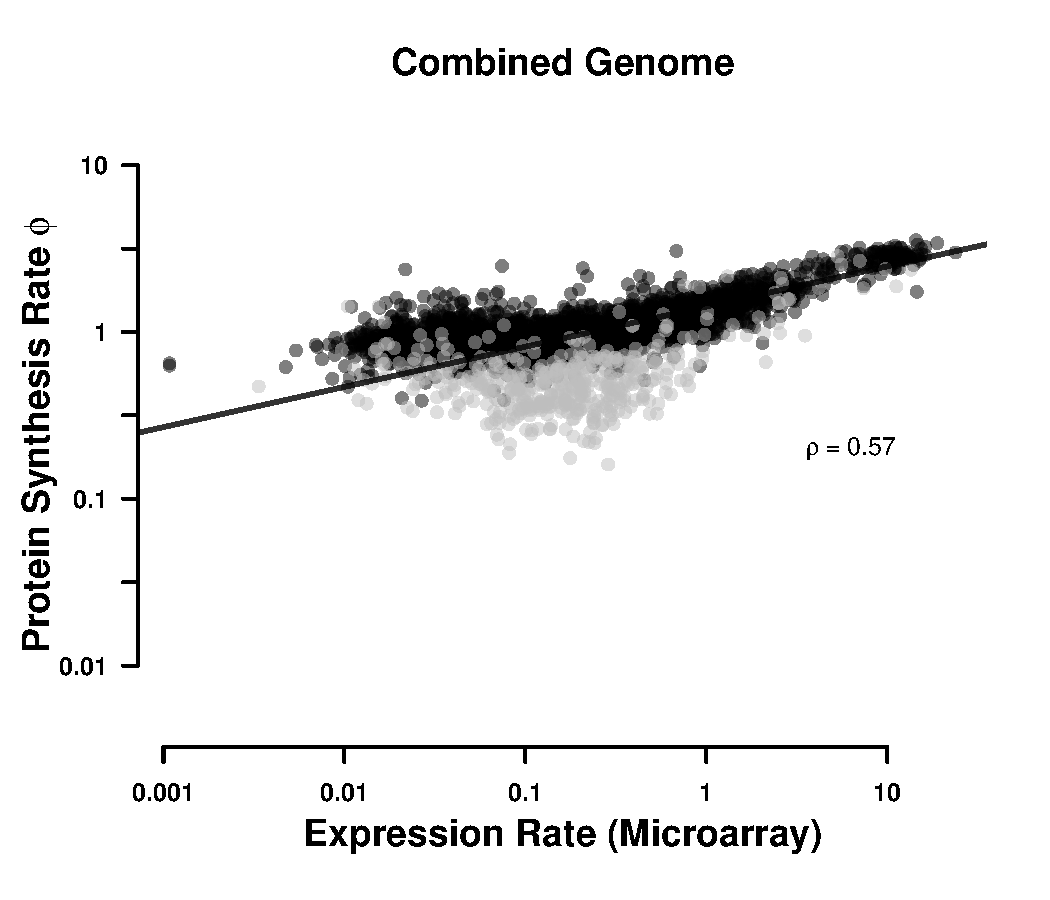
\includegraphics[width=.45\textwidth]{ch3/phi_corr_plot_whole_Genome_estim.pdf}
    \end{subfigure}
    \begin{subfigure}
        \centering
        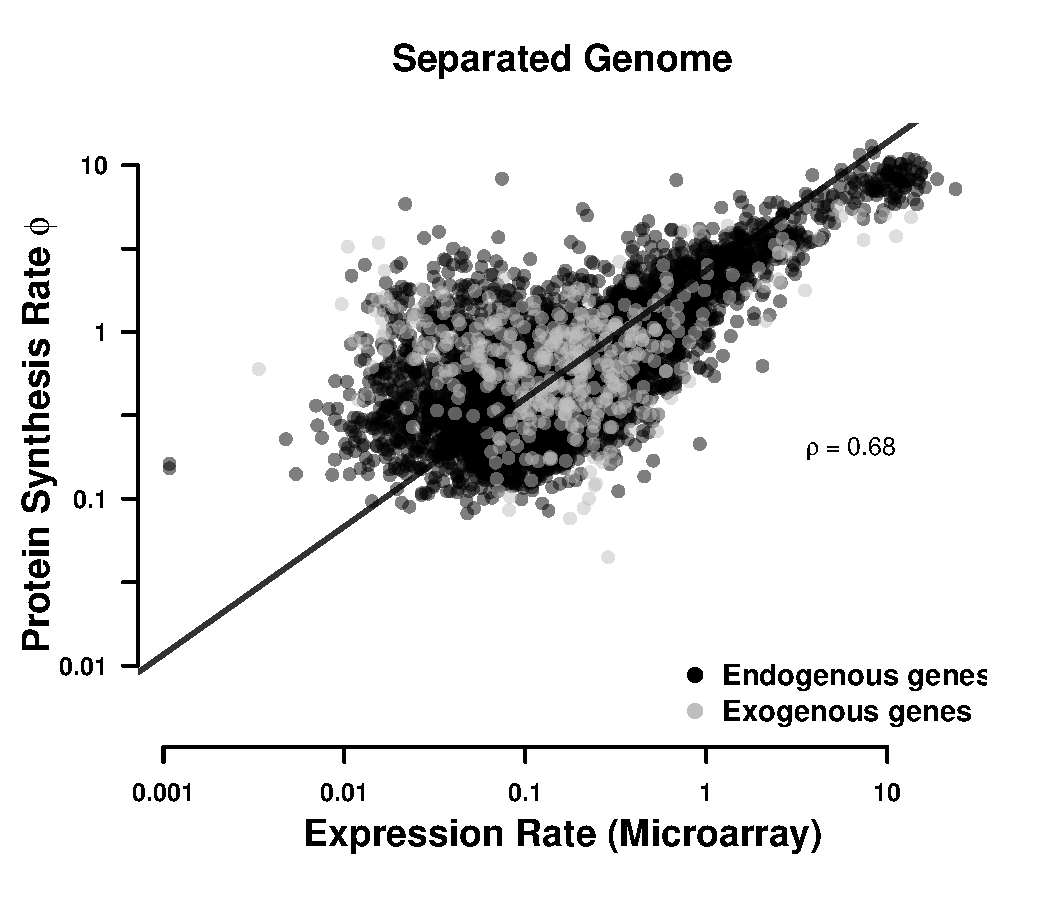
\includegraphics[width=.45\textwidth]{ch3/phi_corr_plot_split_Genome_estim.pdf}
    \end{subfigure}
    \caption{Comparison of predicted protein synthesis rate $\phi$ to Microarray data from \citet{tsankov2010} for (a) the combined genome and (b) the separated endogenous and exogenous genes. 
    Endogenous genes are displayed in black and exogenous genes in gray. Black line indicates type II regression line.}
    \label{fig:phi_corr_two_cond}
\end{figure}

In addition to model selection, we utilized independent information on gene expression to evaluate model fit.
Recognizing differences in \DM and \DE for the endogenous and exogenous gene sets substantially improves our ability to predict protein synthesis rate $\phi$ ($\rho = 0.69$ vs. $\rho = 0.59$ for the full genome;  Figure \ref{fig:phi_corr_two_cond}).

\subsection{Differences in the Endogenous and Exogenous Codon Usage}

As our estimates of parameters for a codon family coding for an amino acid are relative to a reference codon, changes in the reference codon will change the order between sets.
To better compare our estimates of of mutation bias (\DM) and selection bias (\DE) obtained from fitting \ROC between the endogenous and exogenous gene sets, we express our estimates relative to the mean for each codon family.
As 
We find larger differences between \DM than \DE (Figure \ref{fig:csp_comp}). 
Estimates of \DM in the endogenous genes negatively correlate with the \DM estimates for the exogenous genes ($\rho = -0.49$) indicating strong discordance in the mutation environment between \kluyveri and the donor lineage of the exogenous genes.
For example, $\sim 95 \%$ of codon families show mutation preference for A/T ending codons, in contrast, the exogenous genes display an equally strong mutation bias towards C/G ending codons.
Only the two codon amino acid Phenylalanine (Phe, F) shows complete concordance between endogenous and exogenous genes in their \DM values.
\begin{figure}[h]
    \centering
    \begin{subfigure}
        \centering
        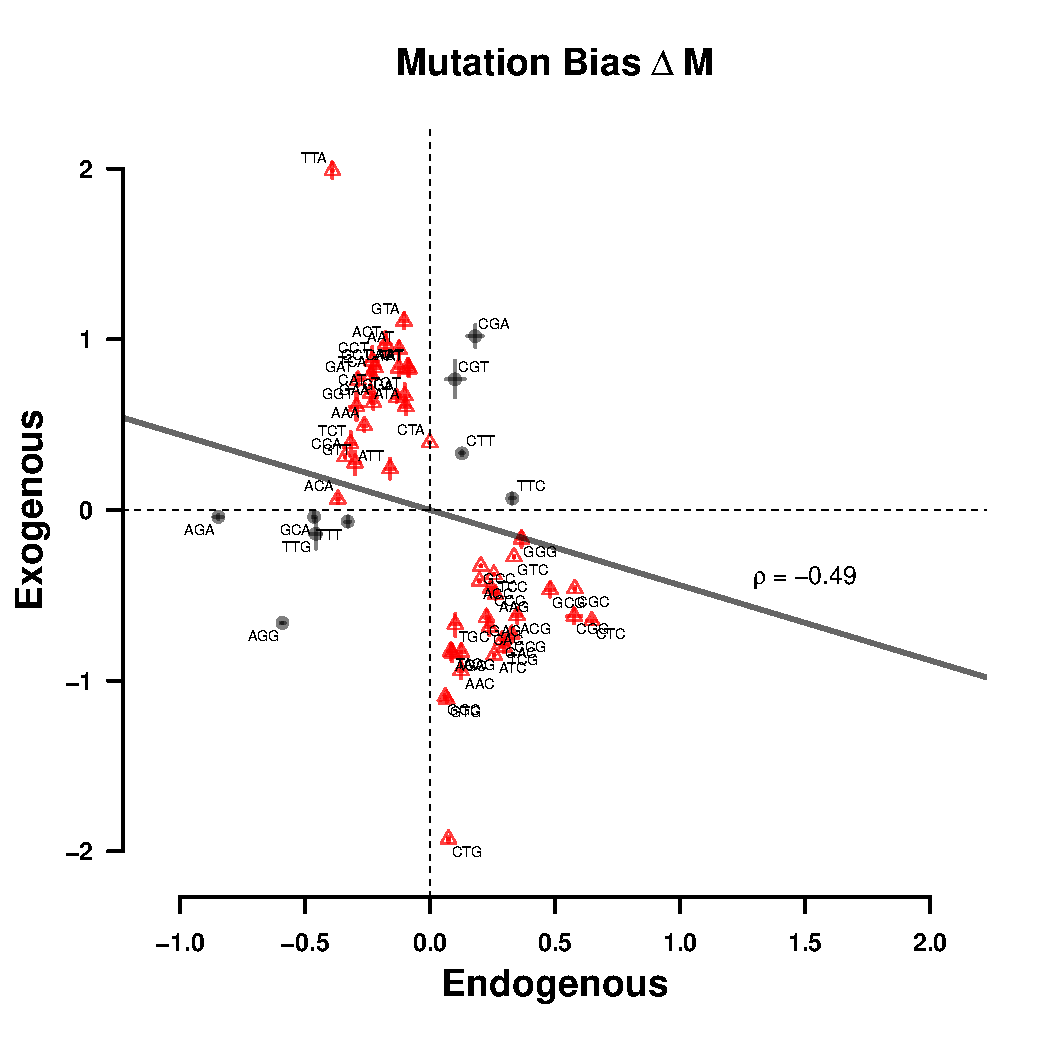
\includegraphics[width=.45\textwidth]{ch3/csp_corr_dm.pdf}
    \end{subfigure}
    \begin{subfigure}
        \centering
        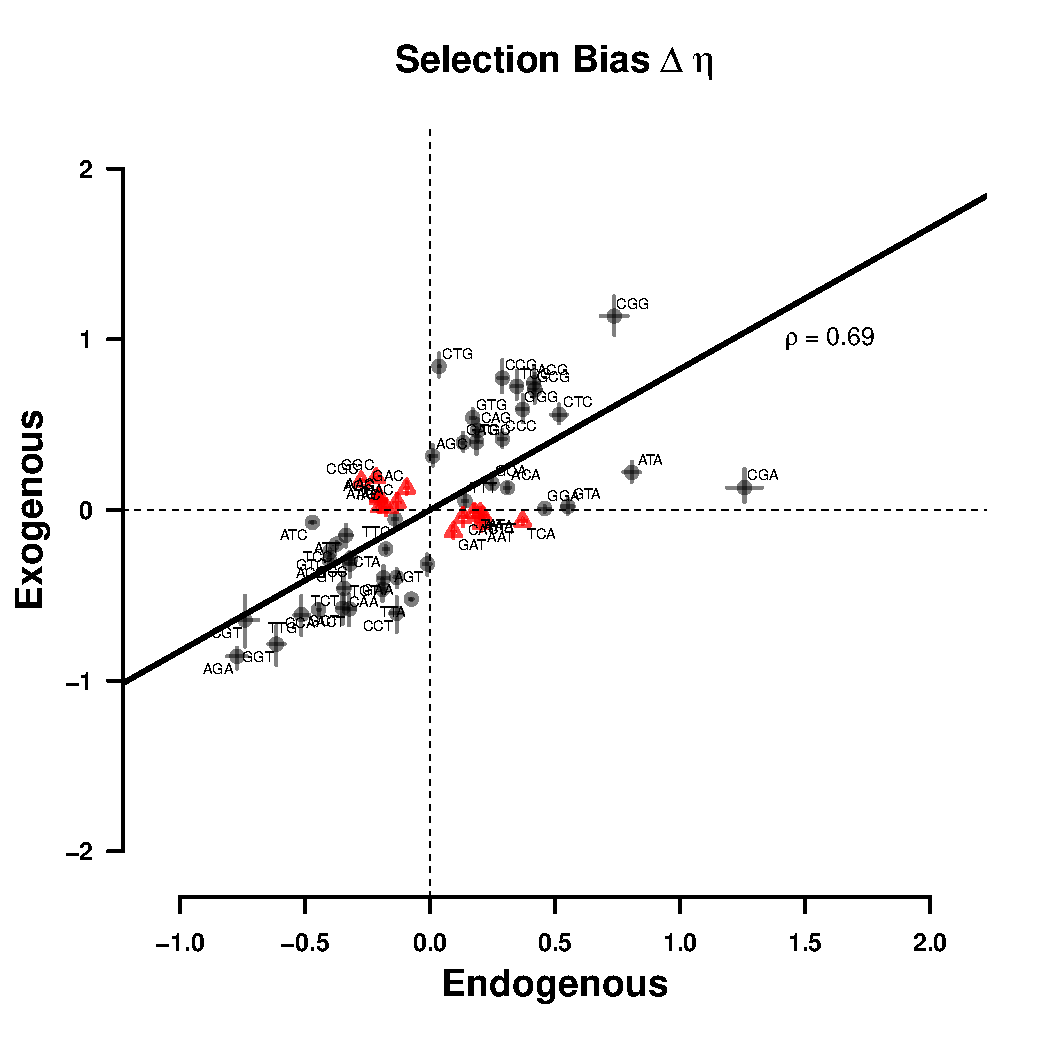
\includegraphics[width=.45\textwidth]{ch3/csp_corr_deta.pdf}
    \end{subfigure}
    \caption{Comparison of (a) mutation bias \DM and (b) selection bias \DE of endogenous and exogenous genes. Estimates are relative to the mean for each codon family. Black dots indicate parameters with sign concordance, red dots indicate parameters with sign discordance between endogenous and exogenous genes. Black line shows the type II regression. Dashed lines mark quadrants.}
    \label{fig:csp_comp}
\end{figure}

Our estimates of \DE for the endogenous and exogenous genes were positively correlated ($\rho = 0.69$), indicating increased concordance of $\sim53\%$ between the two selection environments  (Figure \ref{fig:csp_comp}).
Nevertheless, the endogenous genes only show a selection preference for C and G ending codons in $\sim58\%$ of the codon families.
In contrast, the exogenous genes display a strong preference for A and T ending codons in $\sim89\%$ of the codon families.

The difference in codon preference between endogenous and exogenous genes is striking.
Fits to the complete \kluyveri genome reveal that the relatively small exogenous gene set has a disproportional effect on the model fit.
We find that the complete \kluyveri genome is estimated to share the mutational preference with the exogenous genes in $\sim78\%$ of codon families with discordance between endogenous and exogenous genes.
In two cases, Isoleucine (Ile, I) and Arginine (Arg, R), the strong discrodance in mutation preference results in a estiamted codon preference in the complete \kluyveri genome that is not reflected by either endogenous nor exogenous genes.

The impact of the small exogenous gene set on the fit to the complete \kluyveri genome is less prevalent in our estimates of selection bias $\DE$ but still strong.
We find that the complete \kluyveri genome is estimated to share the selection preference with the exogenous genes in $\sim60\%$ of codon families with discordance between endogenous and exogenous genes.
Therefore, it is important to recognize and treat endogenous and exogenous genes as separate sets to avoid the inference of incorrect synonymous codon preferences.

\subsection{Determining Source of Exogenous Genes}

We combined our estimates of mutation bias ($\Delta M$) and selection bias ($\Delta \eta$) with synteny information and searched for potential source lineages of the introgressed region.
We examined 38 yeast lineages of which two (\textit{Eremothecium gossypii} and \textit{Candida dubliniensis}) showed a strong positive correlation in codon usage (Figure \ref{fig:csp_endo_exo_comp}a).
\begin{figure}[h]
    \centering
    \begin{subfigure}
        \centering
        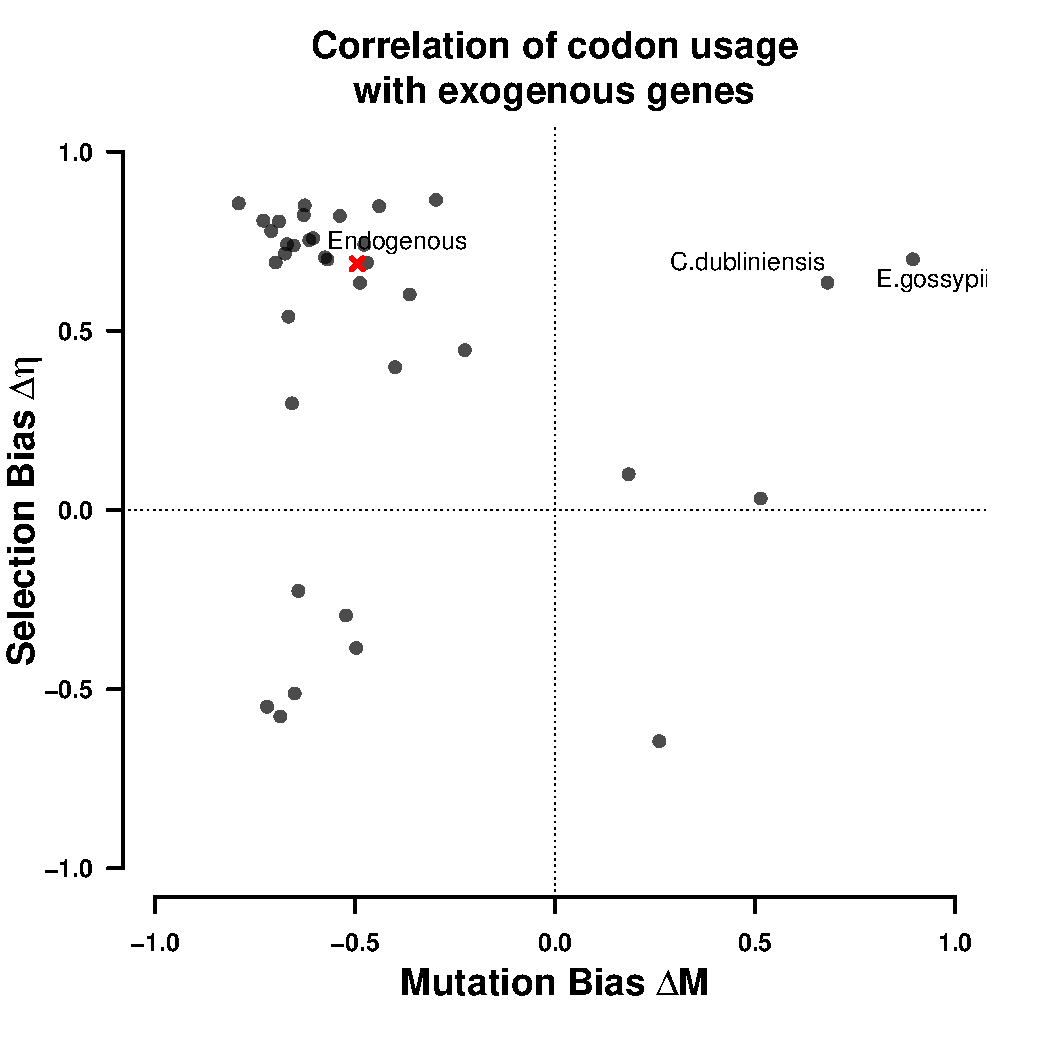
\includegraphics[width=.45\textwidth]{ch3/csp_mean_correlation_exo.pdf}
    \end{subfigure}
    \begin{subfigure}
        \centering
        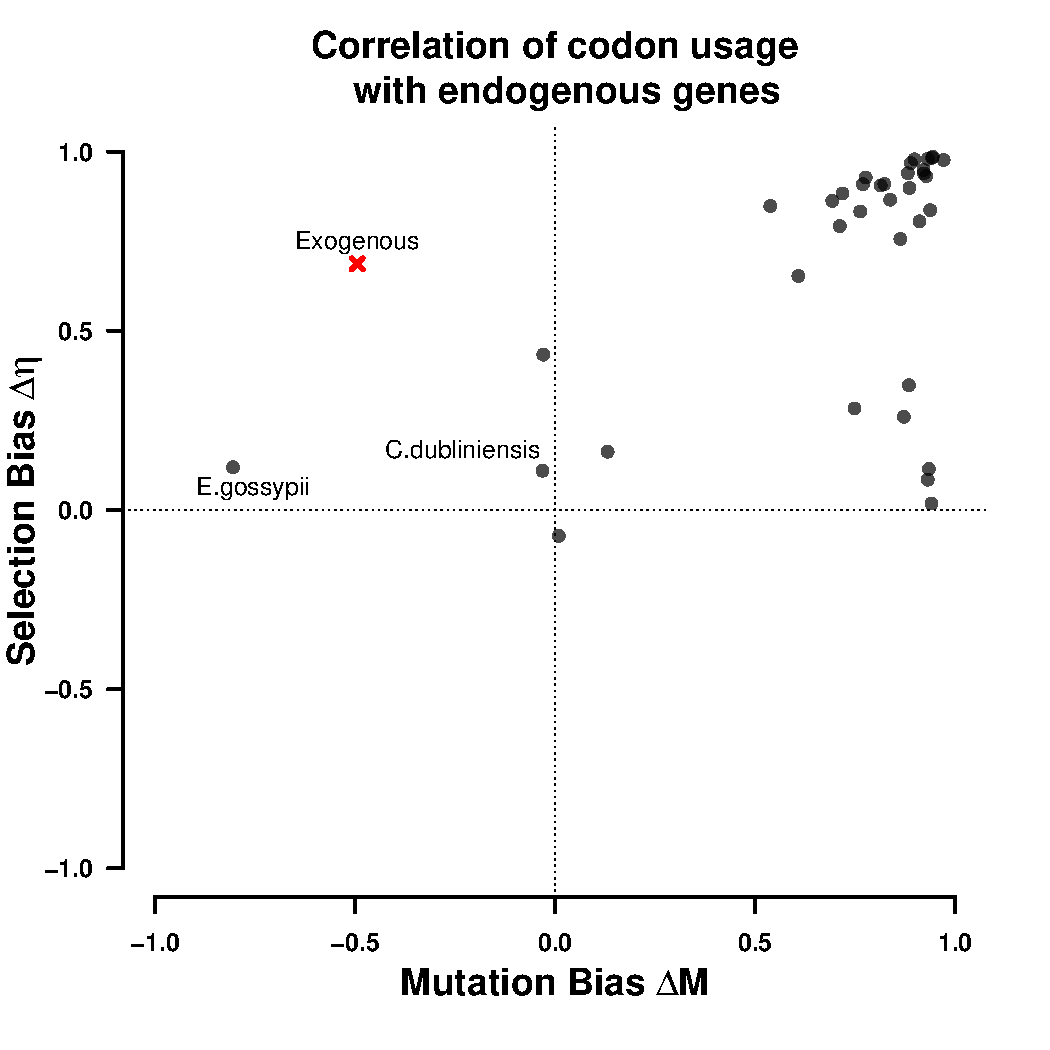
\includegraphics[width=.45\textwidth]{ch3/csp_mean_correlation_endo.pdf}
    \end{subfigure}
    \caption{Correlation of \DM and \DE of the (a) exogenous and (b) endogenous genes with 38 examined yeast lineages. Dots indicate the correlation of \DM and \DE of the lineages with the endogenous and exogenous parameter estimates. All regressions were performed using a type II regression.}
    \label{fig:csp_endo_exo_comp}
\end{figure}
The endogenous \kluyveri genome exhibits codon usage very similar to most yeast lineages examined, indicating little variation in codon usage among the examined yeasts (Figure \ref{fig:csp_endo_exo_comp}b).
Four lineages show a positive correlation for $\Delta M$ and $\Delta \eta$ with the exogenous genes and have a weak to moderate positive correlation in selection bias with the endogenous genes; but, like the exogenous genes, tend to have a negative correlation in $\Delta M$ with the endogenous genes.

Comparing synteny between the exogenous left arm of chromosome C, and \gossypii and \dubl as well as closely related yeast species we find that \gossypii displays the highest synteny coverage  (Figure \ref{fig:synteny_species}a,b).
\dubl, even though it displays similar codon usage does not show synteny with the exogenous region.
Furthermore, the synteny relationship between the exogenous region and other yeasts appears to be limited to the Saccharomycetacease group(Figure \ref{fig:synteny_species}b).
Given these results, we conclude that the \gossypii lineage is the most likely source of the introgressed exogenous genes.

\subsection*{Estimating Introgression Age}

We estimated the introgression assuming that \gossypii is still representative of the mutation bias of its ancestral source lineage at the time of the introgression.
We infer the age of the introgression to be on the order of $6.2\pm1.2\times 10^8$ generations. 
\kluyveri experiences between one and eight generations per day, we therefore expect the introgression to have occurred between $205,000$ to $1,600,000$ years ago.
This estimates the introgression to be older than previous assumed \citet{friedrich2015}.
However, our estimates are likely overestimates as they assume a purely neutral decay.

We also estimated the persistence of the signal of the foreign cellular environment.
Assuming that differences in mutation bias will decay more slowly than differences in selection bias, we predict that the \DM signal of the source cellular environment will have decayed to be within one percent of the \kluyveri environment within about $5.4\pm0.2\times 10^9 $ generations.

\subsection*{Genetic Load of the Exogenous Genes}

Estimates of selection bias for the exogenous genes show that, while well correlated with the endogenous genes, only nine amino acids share the optimal codon.
We therefore expect that the introgressed genes represent a significant reduction in fitness, or genetic load for \kluyveri, and even more so at the time of introgression.
As the introgression occurred before the diversification of \kluyveri and has fixed since then throughout the various populations, we are left without the original chromosome arm \citep{friedrich2015}.
Using our estimates of $\Delta M$ and $\Delta \eta$ from the endogenous genes, we can estimate the genetic load of the exogenous genes relative to an expected gene set.
We define genetic load as the difference between the fitness of an expected, replaced endogenous gene and the inferred introgressed gene relative to drift $s \propto \phi \DE$ (See Methods for details).
\begin{figure}[h]
    \centering
    \begin{subfigure}
        \centering
        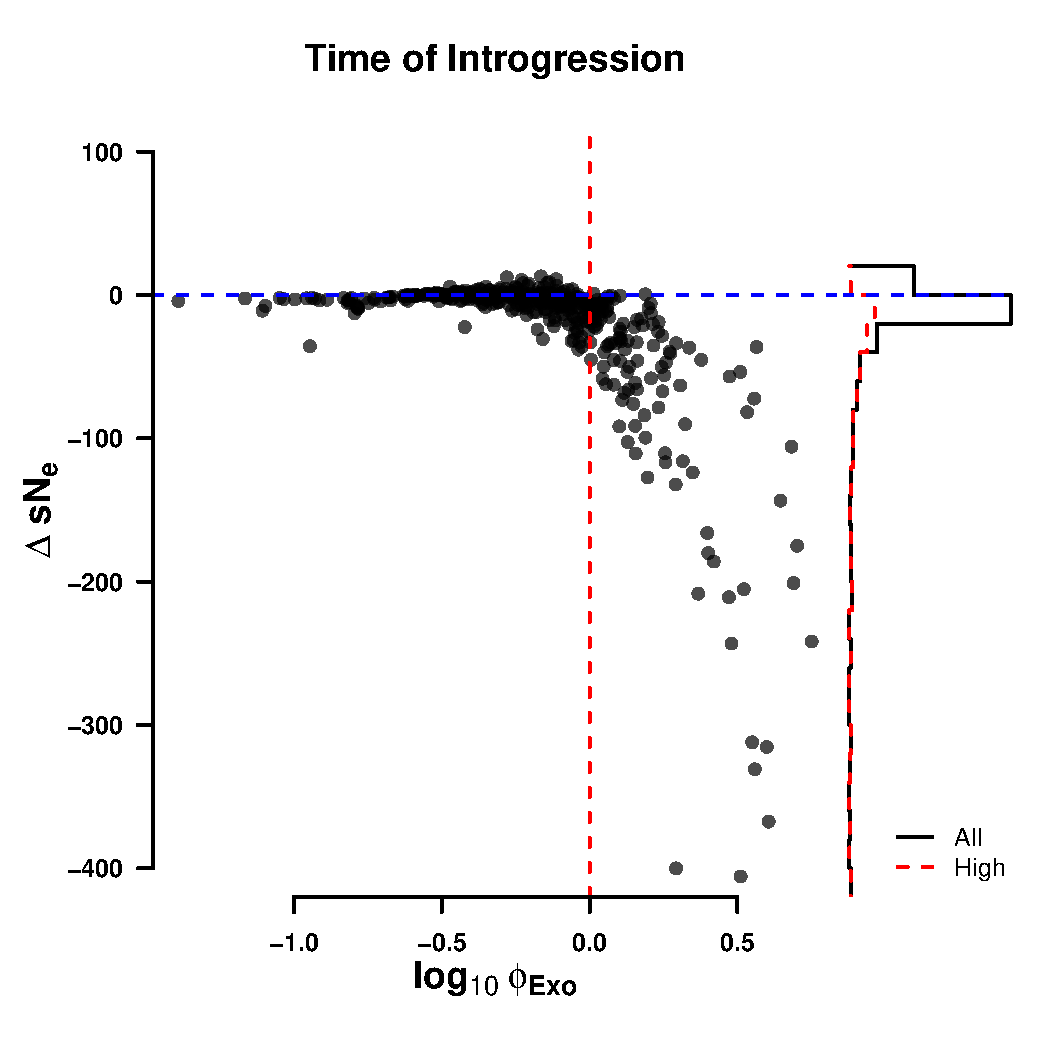
\includegraphics[width=.45\textwidth]{img/fitness_difference_gos_kappa5.pdf}
    \end{subfigure}
    \begin{subfigure}
        \centering
        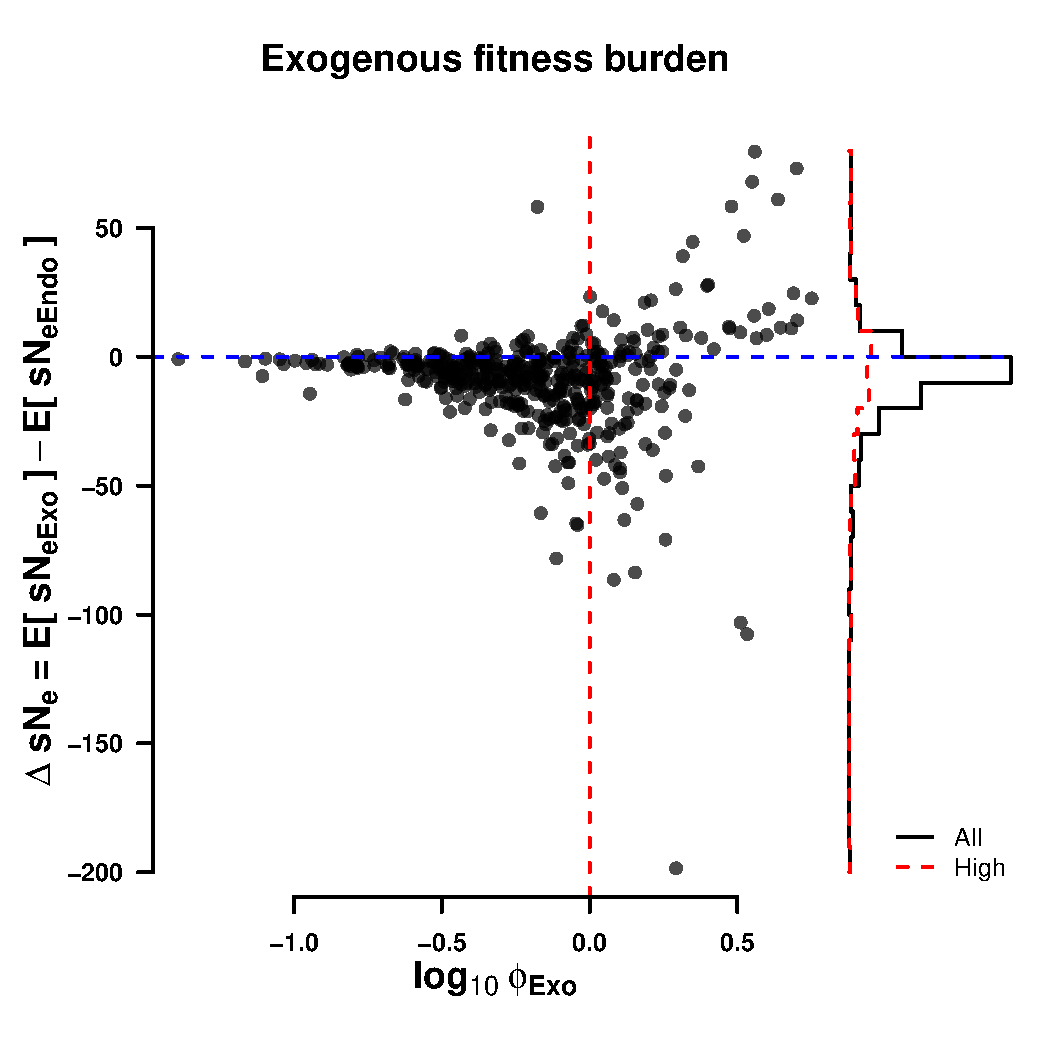
\includegraphics[width=.45\textwidth]{img/fitness_difference_exo.pdf}
    \end{subfigure}
    \caption{Fitness burden $\Delta sN_e$ (a) at the time of introgression ($\kappa = 5$), and (b) currently ($\kappa = 1$). }
    \label{fig:sne_fitness_burden}
\end{figure}

We estimate the genetic load of the exogenous genes at the time of introgression (Figure \ref{fig:sne_fitness_burden}a) and currently (Figure \ref{fig:sne_fitness_burden}b).
As \DE is defined as $\DE = 2N_eq(\eta_i-\eta_j)$, we can not distinguish if $\kappa$ is a scaling on protein synthesis rate $\phi$, effective population size $N_e$ the value of an ATP $q$\citep{gilchrist2015}.

At the time of the introgression, we predict that only a few genes were weakly exapted (Figure \ref{fig:sne_fitness_burden}a) with all high expression genes ($\phi > 1$) being maladapted to the novel cellular environment.
However, these highly expressed genes show the greatest rate of adaptation to the \kluyveri cellular environment (Figures \ref{fig:sne_fitness_burden}a, \ref{fig:adapt_tot}).

\section{Discussion}

Using \ROC we show that the \kluyveri genome contains two distinct signatures of cellular environments, its own endogenous and a foreign exogenous one obtained by an introgression event ($\Delta AIC = 78,000$).
Following \citet{payen2009}, who defined the boundary of the anomalous chromosome region based on its elevated \GC, we partitioned the \kluyveri genome into an endogenous and an exogenous gene set using gene location.
We estimated the codon usage of the entire \kluyveri genome and the separated endogenous and exogenous gene sets (Figure \ref{fig:cub_all_sets}).
Both, Mutation bias and selection bias differ between endogenous and exogenous genes.
The endogenous genes show a strong mutation bias towards A/T ending codons, while the exogenous genes show mutation is bias towards G/C ending codons.
We observed the reversed to be true in selection bias, leading to a strong mismatch in codon usage between the gene sets, supporting our notion of two distinct signatures of codon usage.

Only half of the codon families share the same optimal codon in the endogenous and exogenous gene sets.
However, we find that the strength of selection within a codon family differs between gene sets, causing a change in rank order.
Nevertheless, we find a high correlation for our estimates of selection bias \DE between the two gene sets.
Our estimates of the optimal codon differ in nine cases between endogenous and exogenous genes.
Interestingly, when the difference in codon usage is ignored, we find that in seven out of these nine cases the exogenous codon preference is inferred as optimal(Table \ref{tab:codon_pref_deta}).
We find even greater discordance in our estimates of \DM between endogenous and exogenous gene sets(Table \ref{tab:codon_pref_dm}).
Without recognizing this difference in codon preference our estimates would not have been reflective of the actual codon usage of the \kluyveri genome but of a relatively small introgressed gene set.
This shows that a small number of exogenous genes ($\sim 9 \%$ of genes) can have a disproportional impact on our estimates of \DM and \DE when fitting \ROC to the entire \kluyveri genome.
While this is surprising, it highlights the importance to recognize differences in codon usage within a genome.
Our results also indicate that we can attribute the higher \GC in the exogenous genes mostly to differences in mutation bias favoring G/C ending codons rather than a novel selective force.

Separating the endogenous and exogenous genes improves our estimates of protein synthesis rate $\phi$ by $17 \%$ relative to the full genome estimate ($\rho = 0.59$ vs. $\rho = 0.69$, respectively).
Furthermore, we find that the variation in our estimates of $\phi$ is more consistent with the current understanding of gene expression (compare Figure \ref{fig:phi_corr_two_cond}a and b). 
Small variation in $\phi$ estimates may serve as an indicator for the presents of the signature of multiple cellular environments in future work.
In the case of the \kluyveri genome, finding a severe mismatch in \DM causes $\phi$ values for low expression genes ($\phi < 1$) to increase towards the inflection point where the dominance of mutation gives way to selection.
In the case of the two codon amino acids, the inflection point represents the point at which mutation and selection are contributing equally to the probability of a codons occurrence.
We find this inflection point around $\phi = 1$ for most amino acids (Figure \ref{fig:cub_all_sets}). 
However, \ROC assumes that estimates of $\phi$ follow a log-normal distribution with an expected value $E[\phi] = 1$. 
This assumption allows us to interpret \DE as the strength of selection relative to drift ($sN_e$) for a codon in a gene with the average protein synthesis rate $\phi = 1$.
However, tying the mean and standard deviation of the prior distribution together.
Therefore, an increase in $\phi$ for low expression genes has to be meet with a decrease of $\phi$ for high expression genes, reducing the overall variance in $\phi$ (see \citet{gilchrist2015} for details). 

Having shown that the introgressed exogenous genes reflect a foreign cellular environment, we used the quantitative estimates of mutation bias \DM and selection bias \DE from \ROC to identify potential source lineages.
The comparison of the endogenous and exogenous \DM and \DE estimates to 38 other yeast lineages revealed that most yeasts examined share similarity in mutation bias (Figure \ref{fig:csp_comp}).
Similar, we find strong similarities in selection bias between examined yeasts, potentially indicating stabilizing selection on codon usage.
However, the exogenous genes do not share this commonality (Figure \ref{fig:csp_comp}a), as their mutation bias strongly deviates from the endogenous genes and most other yeast species examined. 
This large difference in mutation bias between endogenous and exogenous genes allowed us to limit our candidate list to only two likely lineages, \dubl and \gossypii.
Interestingly, we did not find \textit{Lachancea thermotolerance}, a thermophilic lineage closely related to \kluyveri, as a potential candidate.
While \textit{L. thermotolerance} does have a strong synteny relationship with \kluyveri, it does not show similarity in codon usage with the exogenous genes and does not share their high \GC.

Inference of synteny relationships between the exogenous region and \dubl and \gossypii as well as closely related species showed that synteny relationship is limited to the Saccharomycetaceae clade (Figure \ref{fig:synteny_species}b).
\gossypii showed the highest syntenty coverage and is the only species with similar codon usage.
Furthermore, \gossypii is the only species examined with a \GC $> 50 \%$ like it is observed in the exogenous region.
The synteny coverage extends along the whole exogenous regions with the exception to the very 3' and 5' end of the region. 
The lack of synteny at the ends of the region also coincides with a drop in \GC, potentially indicating remains of the original replaced region or increased adaptation.
The ancestral introgressed region may have also broken up in \gossypii as we find non overlapping synteny with chromosomes \emph{VI} and \emph{V} as well as have indication that the C chromosome of \kluyveri very robust to recombination events \citep{payen2009, vakirlis2016}. 

With \gossypii identified as potential source lineage of the introgressed region, we inferred the time past since the introgression occurred using our estimates of mutation bias \DM.
The \DM estimates are well suited for this task as they are free of the influence of selection and unbiased by $N_e$ and other scaling terms, which is in contrast to our estimates of \DE \citep{gilchrist2015}.
We estimated the time since introgression to be on the order of $6\times 10^8$ generations, which is $\sim 10$ times longer time than a previous estimate by \citet{friedrich2015} of a minimum of $5.6\times 10^7$ generations .
However, our estimate implicitly assumes all mutations are neutral, it is therefore a conservative estimate, potentially overestimating the time since introgression. 
Our estimate also depend on the assumption that the \gossypii cellular environment reflects the ancestral environment at the time of the introgression.
If the the ancestral mutation environment was more similar to the \kluyveri environment at the time of the introgression than the \gossypii environment is today, we would overestimate this time.
On the other hand, we would underestimate the time since introgression if the two cellular environments were more dissimilar.
We could have attempted to reconstruct the ancestral state of \gossypii, however, as methods for ancestral state reconstruction are phenomenological, assumptions would be unclear. 

The estimates of mutation bias \DM also allow us the infer the time until the signature of the exogenous cellular environment will have decayed to be indistinguishable at about one percent difference.
Our estimate of decay is an order of magnitude greater than our estimate of the time since introgression ($5\times 10^9$ and $6\times 10^8$ generations).
Estimates of decay based on \DM are more conservative as we expect differences in \DE to decay before due to selection favoring the decay.
 
As we have determined that the introgression event has a long persisting exogenous signature, it is important to understand the fitness consequences of such an event.
We estimated the genetic load that the exogenous genes represent assuming that the replaced endogenous genes and the new exogenous genes had the same amino acid composition.
This assumption, along with the assumption that the current \kluyveri cellular environment is reflective of the cellular environment at the time of the introgression is necessary to estimate the expected endogenous sequence that was replaced.
Our results show that individual low expression genes contribute little to the genetic load, and show less adaptation to the novel cellular environment (Figure \ref{fig:sne_fitness_burden}, \ref{fig:adapt_tot}).
A small number of low expression genes even appear exapted, likely due to the mutation bias in the endogenous genes matching the selection bias in the exogenous genes for G/C ending codons.
Highly expressed genes on the other hand have greatly adapted to the \kluyveri cellular environment.
This, however, does not mean that these genes show a higher rate of evolution, but that small changes in their sequence have large impacts on the fitness burden these sequences represent.
To this day, the exogenous genes represent a significant fitness burden on \kluyveri.
However, our estimates are conservative as we do not account for potential changes in the codon usage of \gossypii. 
While divergent evolution in codon usage between \gossypii and \kluyveri would cause us to overestimate the genetic load, convergent evolution, on the other hand, would cause us to underestimate the genetic load.
However, as the introgression appears to have reached fixation \citep{friedrich2015}, the genetic load relative to the replaced chromosome arm is only of theoretical interest.

The large genetic load the exogenous genes represented at the time of the introgression indicates that the fixation of the introgression was a very unlikely event in a population with a large $N_e$ as it is typical for yeasts.
It is hard to contextualize the probability of this introgression being fixed as we are not aware of any estimates of the frequency at which such large scale introgressions of genes with very different signatures of codon usage occur.
One example is \textit{Saccharomyces bayanus}, a hybrid of \textit{Saccharomyces uvarum},\textit{Saccharomyces cerevisiae}, and \textit{Saccharomyces eubayanus}.
However, unlike with \kluyveri and \gossypii it appears that the donor lineages show similar codon usage.
\textit{Saccharomyces cerevisiae} and \textit{Saccharomyces eubayanus} show a very strong correlation between selection bias \DE of $\rho = 0.98$ and a strong correlation between mutation bias \DM of $ \rho = 0.83$
We were unable to identify codon usage for \textit{Saccharomyces uvarum}.
However, \kluyveri diverged about 85 Mya ago from the rest of the Lachancea clade.
This represents between $10^{10}$ to $10^{11}$ generations.
Assuming for yeasts typical effective population size on the order of $10^8$, we are left with $10^{18}$ to $10^{19}$ opportunities for such an event to occur.
In addition, the strong mutation bias towards G/C ending codons in the exogenous genes may have contributed to the fixation of this introgression (include figure of \DM v \DE).
It is, on the other hand, also possible that despite their mismatch in codon usage, the exogenous genes have represented a fitness increase due to external environmental factors resulting in the fixation of the introgression.
 
In conclusion, our results show the usefulness of the separation of mutation bias and selection bias and the importance of recognizing the presence of multiple cellular environments in the study of codon usage.
We also illustrate how a mechanistic model like \ROC and the quantitative estimates it provides can be used for more sophisticated hypothesis testing in the future.
In contrast to other approaches used to study codon usage like CAI \citep{sharp1987} or tAI \citep{dosreis2004}, \ROC is sensitive to differences in mutation bias.
We highlight potential pitfalls when estimating codon preferences, as estimates can be biased by the signature of a second, historical cellular environment.
In addition, we show how quantitative estimates of mutation bias and selection relative to drift can be obtained from codon data and used to infer the fitness cost of an introgression as well as its history and potential future.


\section{Materials and Methods}

\subsection{Separating endogenous and exogenous genes}
A GC-rich region was identified by \citet{payen2009} in the \kluyveri genome extending from position 1 to 989,693 of chromosome C.
This region was later identified as an introgression by \citet{friedrich2015}.
We obtained the \kluyveri genome from SGD Project \url{http://www.yeastgenome.org/download-data/} (last accessed: 09-27-2014) and the annotation for \kluyveri NRRL Y-12651 (assembly ASM14922v1) from NCBI (last accessed: 12-09-2014).
We assigned 457 genes located on chromosome C with a location within the $\sim 1 Mb$ window to the exogenous gene set.
All other 4864 genes of the \kluyveri genome were assigned to the exogenous genes.
All genes could be uniquely assigned to one or the other gene set.

\subsection{Model Fitting with \ROC}
\ROC was fitted to each genome using AnaCoDa (0.1.1) \citep{landerer2018} and R (3.4.1).
\ROC was run from multiple starting values for at least 250,000 iterations, every 50th sample was collected to reduce autocorrelation. 
After manual inspection to verify that the MCMC had converged, parameter posterior means were estimated from the last 500 samples.

\subsection{Comparing codon specific parameter estimates}
Choice of reference codon does reorganize codon families coding for an amino acid relative to each other, therefore all parameter estimates are relative to the mean for each codon family.
\begin{equation}
\DM_{i,a}^c = \DM_{i,a} - \bar{\DM_a}
\end{equation}
\begin{equation}
\DE_{i,a}^c = \DE_{i,a} - \bar{\DE_a}
\end{equation}
Comparison of codon specific parameters (\DM and \DE) was performed using the function lmodel2 in the R package lmodel2 (1.7.3) and R version 3.4.1.
Type II regression was performed with re-centered parameter estimates, accounting for noise in dependent and independent variable.


\subsection{Synteny}
We obtained complete genome sequences from NCBI (last accessed: 02-05-2017).
Genomes were aligned and checked for synteny using SyMAP (4.2) with default settings \citep{soderlund2006, soderlund2011}.
We assessed Synteny as percentage non-overlapping coverage of the exogenous gene region (Figure \ref{fig:synteny_species}b).

\subsection{Determining introgression timeline}
We modeled the change in codon frequency over time using an exponential model for all two codon amino acids, and describing the change in codon $c_1$ as
\begin{equation}
\frac{d c_1}{d t} = -\mu_{1,2}c_1 - \mu_{2,1}(1-c_1)
\label{mut_ode}
\end{equation}
where $\mu_{i,j}$ is the rate at which codon $i$ mutates to codon $j$ and $c_1$ is the frequency of the reference codon.
Our estimates of $\DM_{endo}$ can be directly related to the steady state of equation \ref{mut_ode}.
\begin{equation}
\frac{\mu_{2,1}}{\mu_{1,2} + \mu_{2,1}} = \frac{1}{1+\exp(\DM_{endo})}
\end{equation}
Solving for $\mu_{1,2}$ gives us $\mu_{1,2} = \DM_{endo}\exp(\mu_{2,1})$ which allows us to rewrite and solve equation \ref{mut_ode} as
\begin{equation}
c_1(t) = \frac{\exp(-t(1+\DM_{endo})\mu_{2,1})\exp(t(1+\DM_{endo})\mu_{2,1}) + (1+\DM_{endo})K}{1+\DM_{endo}}
\label{mut_close_form}
\end{equation}
where K is
\begin{equation}
K = \frac{-1 + c_1(0) + c_1(0)\DM_{endo}}{1+\DM_{endo}}
\end{equation}

Equation \ref{mut_close_form} was solved over time with a mutation rate $m_{2,1}$ of $3.8\times 10^{-10}$ per nucleotide per generation \citep{lang2008}. 
Initial codon frequencies $c_1(0)$ for each codon family where taken from our estimates of $\DM_{gos}$ from \gossypii. 
Current codon frequencies for each codon family where taken from our estimates of \DM from the exogenous genes.
Mathematica (9.0.1.0) \citep{Mathematica} was used to calculate the time $t_{exo}$ it takes for the initial codon frequencies $c_1(0)$ for each codon family to change to the current exogenous codon frequencies.
The same equation was used to determine the time $t_{endo}$ at which the signal of the exogenous cellular environment has decayed to within $1 \%$ of the endogenous environment.

\subsection*{Estimating Genetic Load}

To estimate the fitness burden, we made three key assumptions.
First, we assumed that the current exogenous amino acid composition of genes is representative of the replaced endogenous genes.
Second, we assume that the currently observed cellular environment of \gossypii reflects the cellular environment that the exogenous genes experienced before transfer to \kluyveri.
Lastly, we assume that the difference in the efficacy of selection between the cellular environments of the source lineage and \kluyveri can be expressed as a scaling constant and that protein synthesis rate $\phi$ has not changed between the replaced endogenous and the introgressed exogenous genes.

Using estimates for $N_e$ from XXX et al. we scale our estimates of \DE and define $\DE' = \frac{\DE}{N_e}$.
We calculated the fitness burden each gene represents assuming additive fitness effects as 
\begin{equation}
s_g = \sum_i^{C} -\kappa \phi_g \DE'_i n_{g,i} 
\end{equation}
where $s_g$ is the selection against translation inefficiency.
$\phi_g$ is the estimated protein synthesis rate for gene $g$ in the exogenous gene set.
$n_{g,i}$ is the codon count of each codon $i$ in the codon set $C$ for each gene $g$.
$\kappa$ is a constant, scaling the efficacy of selection between cellular environments.
Like stated previously, our \DE are relative to the mean of the codon family.
We find that the fitness burden of the introgressed genes  is minimized at $\kappa \sim 5$ (Figure \ref{fig:sne_scaling}b).
Thus, we set $\kappa = 1$ if we calculate the $s_g$ for the endogenous and the current exogenous genes, and $\kappa = 5$ for $s_g$ for the fitness burden at the time of introgression.
Since we are unable to observe codon counts for the replaced endogenous genes and for the exogenous genes at the time of introgression, we calculate expected codon counts
\begin{equation}
E[n_{g,i}] = \frac{\exp(-\DM_i -\DE_i\phi_g)}{\sum_j^C \exp(-\DM_j -\DE_j\phi_g)}\times m_{a_i}
\end{equation} 
$m_{a_i}$ is the number of occurrences of amino acid $a$ that codon $i$ codes for.

We report the genetic load of the introgression as $\Delta s = s_{Intro} - s_{Endo}$ where $s_{Intro}$ is either the fitness burden at the time of the introgression or presently.

\section{Acknowledgments}

This work was supported in part by NSF Awards MCB-1120370 (MAG and RZ) and DEB-1355033 (BCO, MAG, and RZ) with additional support from The University of Tennessee Knoxville. 
CL received support as a Graduate Student Fellow at the National Institute for Mathematical and Biological Synthesis, an Institute sponsored by the National Science Foundation through NSF Award DBI-1300426, with additional support from UTK. 
The authors would like to thank Brian C. O'Meara and Alexander Cope for their helpful criticisms and suggestions for this work.


\bibliographystyle{unsrtnat}
\bibliography{kluyveri_paper}

\clearpage
\section{Supplementary Material}
\beginsupplement

Supporting Materials for \emph{Fitness consequences of mismatched codon usage} \ by Landerer \emph{et al.}.


\begin{table}
    \centering
\begin{tabular}{  l  c  c  c  c  }
\hline
	Amino Acid & \gossypii & Endogenous & Exogenous & \kluyveri \\ \hline \hline
	Ala A & GCG & GCA & GCG & GCG \\ \hline
	Cys C & TGC & TGT & TGC & TGC \\ \hline
	Asp D & GAC & GAT & GAC & GAC \\ \hline
	Glu E & GAG & GAA & GAG & GAG \\ \hline
	Phe F & TTC & TTT & TTT & TTT \\ \hline
	Gly G & GGC & GGT & GGC & GGC \\ \hline
	His H & CAC & CAT & CAC & CAC \\ \hline
	Ile I & ATC & ATT & ATC & ATA \\ \hline
	Lys K & AAG & AAA & AAG & AAA \\ \hline
	Leu L & CTG & TTG & CTG & CTG \\ \hline
	Asn N & AAC & AAT & AAC & AAT \\ \hline
	Pro P & CCG & CCA & CCG & CCG \\ \hline
	Gln Q & CAG & CAA & CAG & CAG \\ \hline
	Arg R & CGC & AGA & AGG & CGG \\ \hline
	Ser$_4$ S & TCG & TCT & TCG & TCG \\ \hline
	Thr T & ACG & ACA & ACG & ACG \\ \hline
	Val V & GTG & GTT & GTG & GTG \\ \hline
	Tyr Y & TAC & TAT & TAC & TAC \\ \hline
	Ser$_2$ Z & AGC & AGT & AGC & AGC \\ \hline
\end{tabular}
    \caption{Synonymous codon preference in the various data sets based on our estimates of $\Delta M$}
    \label{tab:codon_pref_dm}
\end{table}

\clearpage

\begin{table}
    \centering
\begin{tabular}{  l  c  c  c  c  }
\hline
	Amino Acid & \gossypii & Endogenous & Exogenous & \kluyveri \\ \hline \hline
	Ala A & GCT & GCT & GCT & GCT \\ \hline
	Cys C & TGT & TGT & TGT & TGT \\ \hline
	Asp D & GAT & GAC & GAT & GAT \\ \hline
	Glu E & GAA & GAA & GAA & GAA \\ \hline
	Phe F & TTT & TTC & TTC & TTC \\ \hline
	Gly G & GGA & GGT & GGT & GGT \\ \hline
	His H & CAT & CAC & CAT & CAT \\ \hline
	Ile I & ATA & ATC & ATT & ATT \\ \hline
	Lys K & AAA & AAG & AAA & AAG \\ \hline
	Leu L & TTA & TTG & TTG & TTG \\ \hline
	Asn N & AAT & AAC & AAT & AAC \\ \hline
	Pro P & CCA & CCA & CCT & CCA \\ \hline
	Gln Q & CAA & CAA & CAA & CAA \\ \hline
	Arg R & AGA & AGA & AGA & AGA \\ \hline
	Ser$_4$ S & TCA & TCC & TCT & TCT \\ \hline
	Thr T & ACT & ACC & ACT & ACT \\ \hline
	Val V & GTT & GTC & GTT & GTT \\ \hline
	Tyr Y & TAT & TAC & TAT & TAC \\ \hline
	Ser$_2$ Z & AGT & AGT & AGT & AGT \\ \hline
\end{tabular}
    \caption{Synonymous codon preference in the various data sets based on our estimates of $\Delta \eta$}
    \label{tab:codon_pref_deta}
\end{table}

\clearpage
\begin{figure}[H]
     \centering
	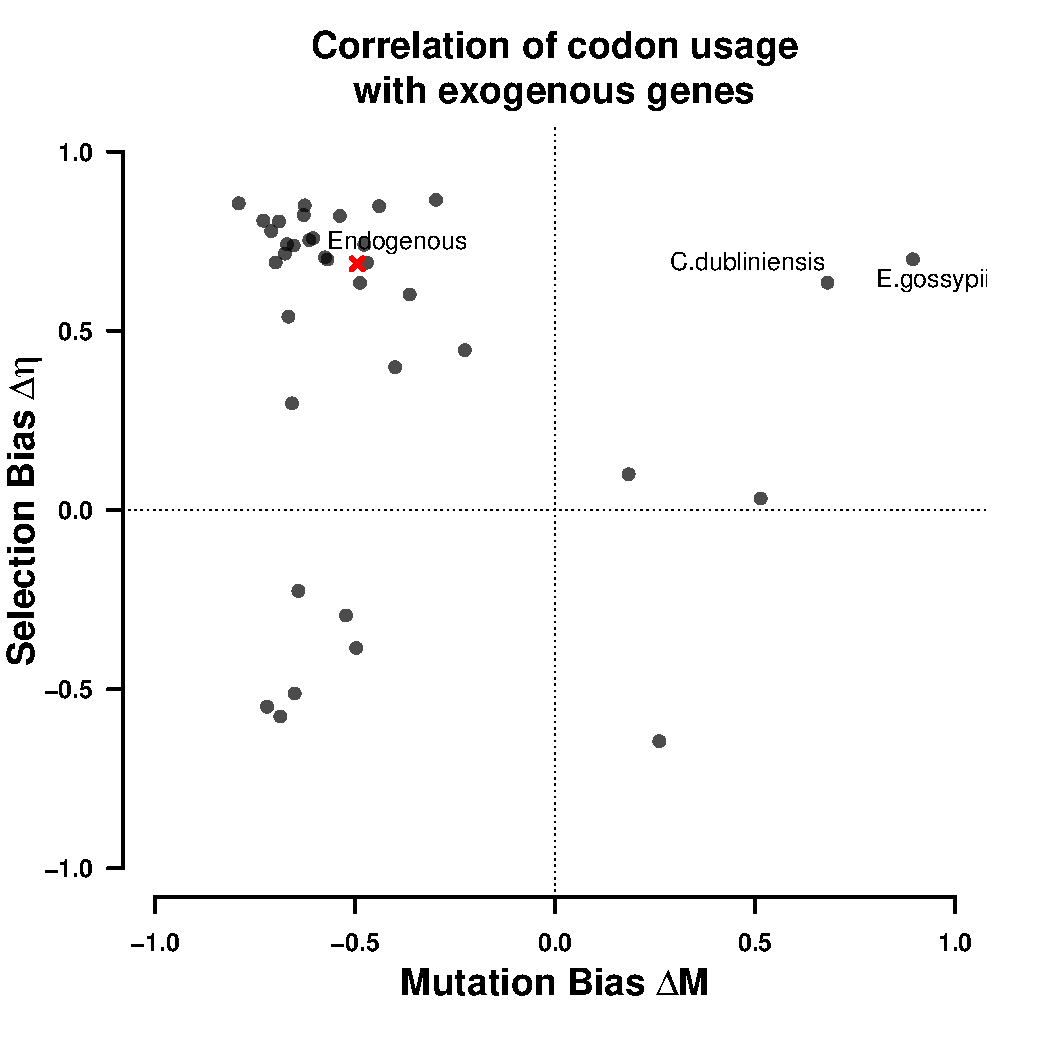
\includegraphics[width=0.5\textwidth]{ch3/csp_mean_correlation_exo.pdf}
	\caption{Correlation of \DM and \DE of the endogenous genes with 38 examined yeast lineages. Dots indicate the correlation of \DM and \DE of the lineages with the endogenous and exogenous parameter estimates. All regressions were performed using a type II regression.}
	\label{fig:csp_endo_comp}
\end{figure}


\begin{figure}[H]
     \centering
	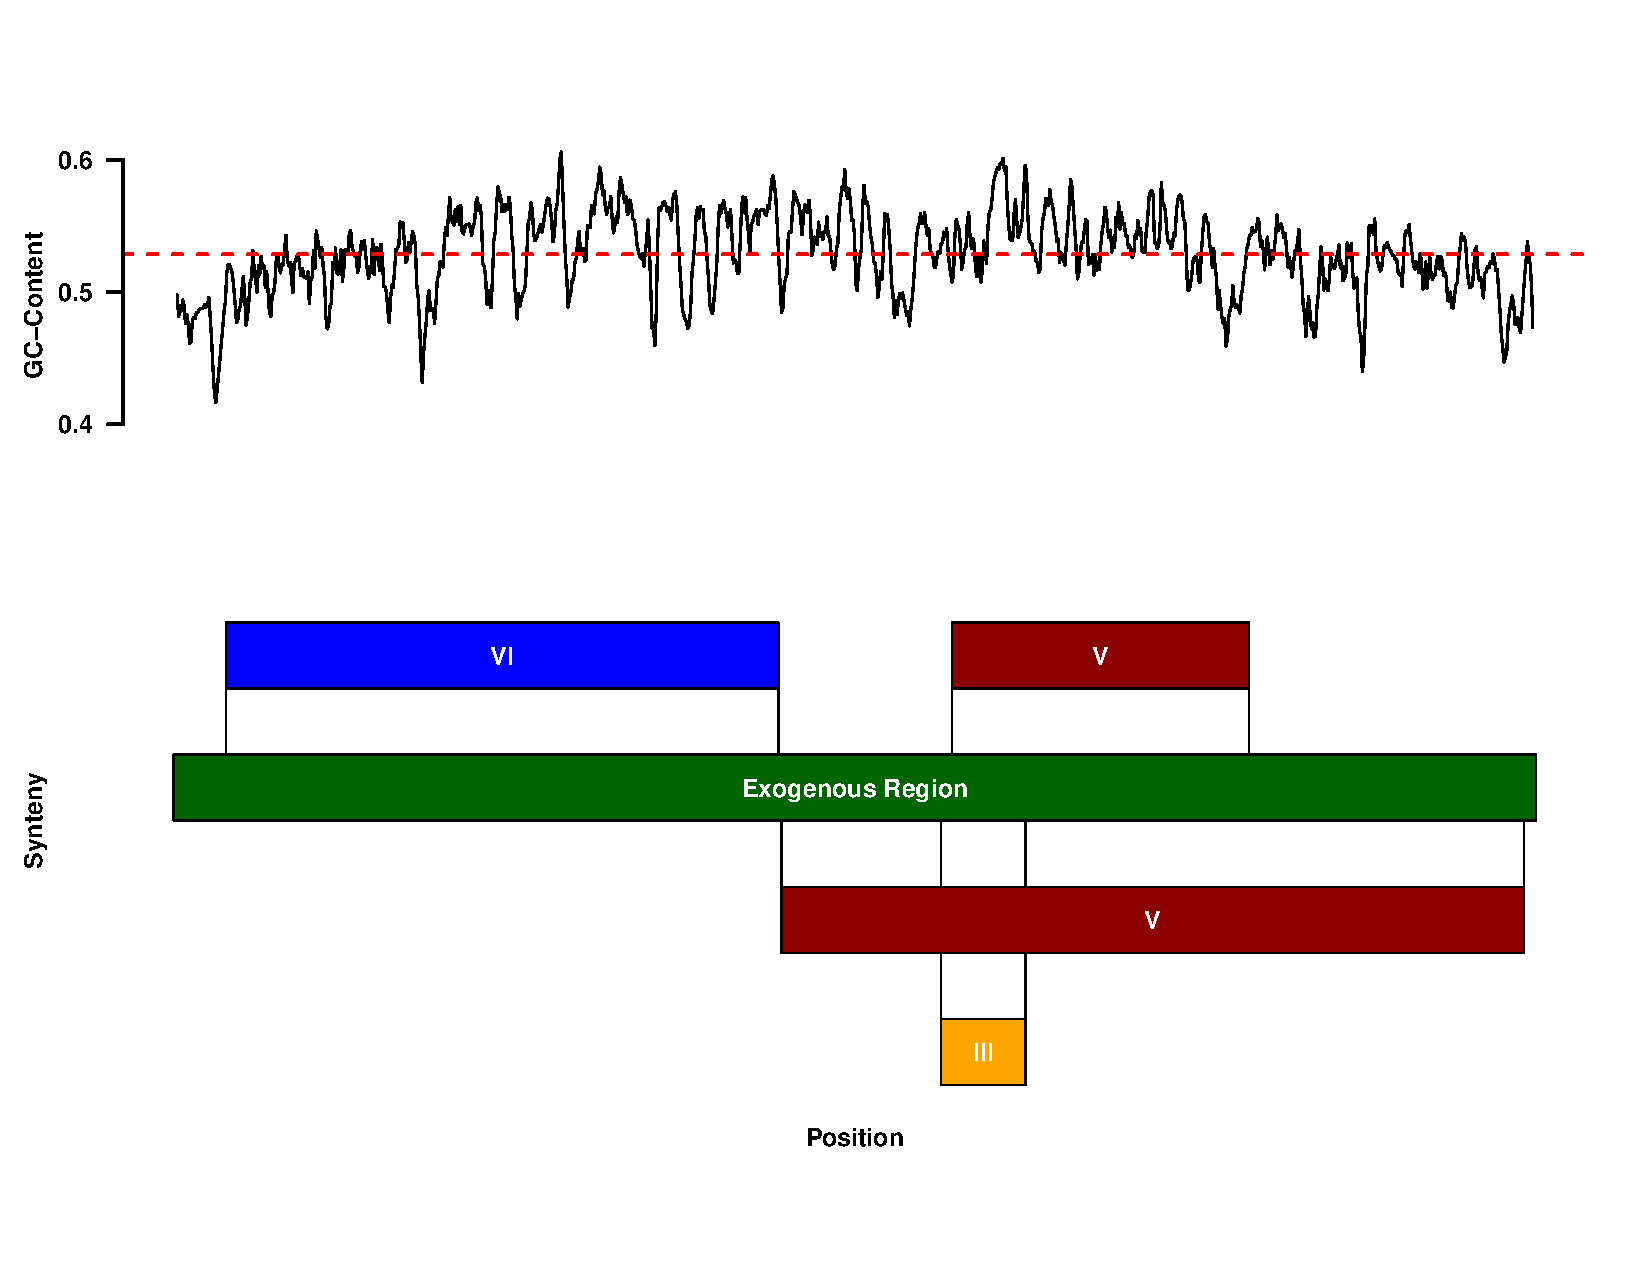
\includegraphics[width=0.5\textwidth]{ch3/synteny_blocks_and_gc.pdf}
	\caption{Synteny relationship of \gossypii and the exogenous genes}
	\label{fig:synt_rel}
\end{figure}


\begin{figure}[H]
     \centering
	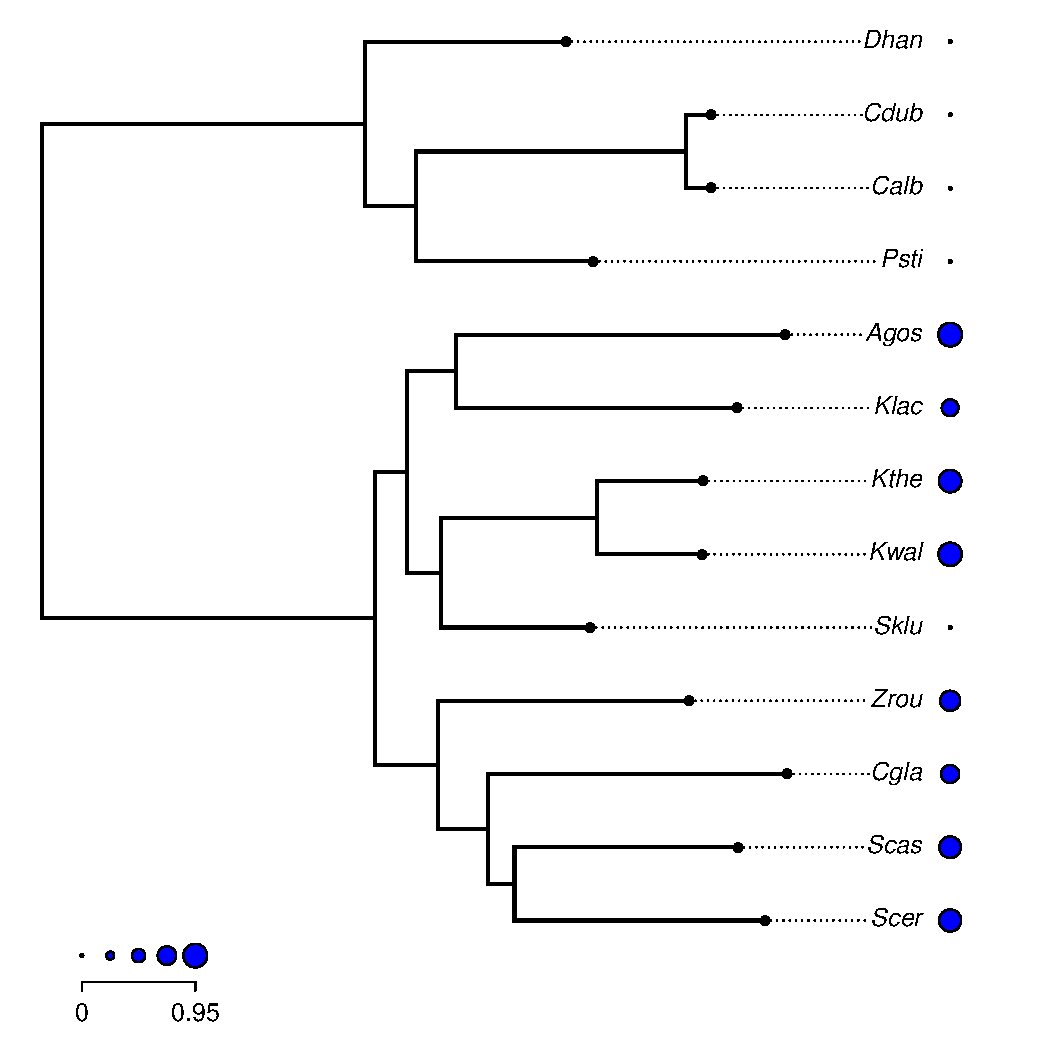
\includegraphics[width=0.5\textwidth]{ch3/synteny_coverage.pdf}
	\caption{Amount of synteny for each species (Units of std dev) checked for synteny.}
	\label{fig:synteny_species}
\end{figure}



\begin{figure}[h]
    \centering
    \begin{subfigure}
        \centering
        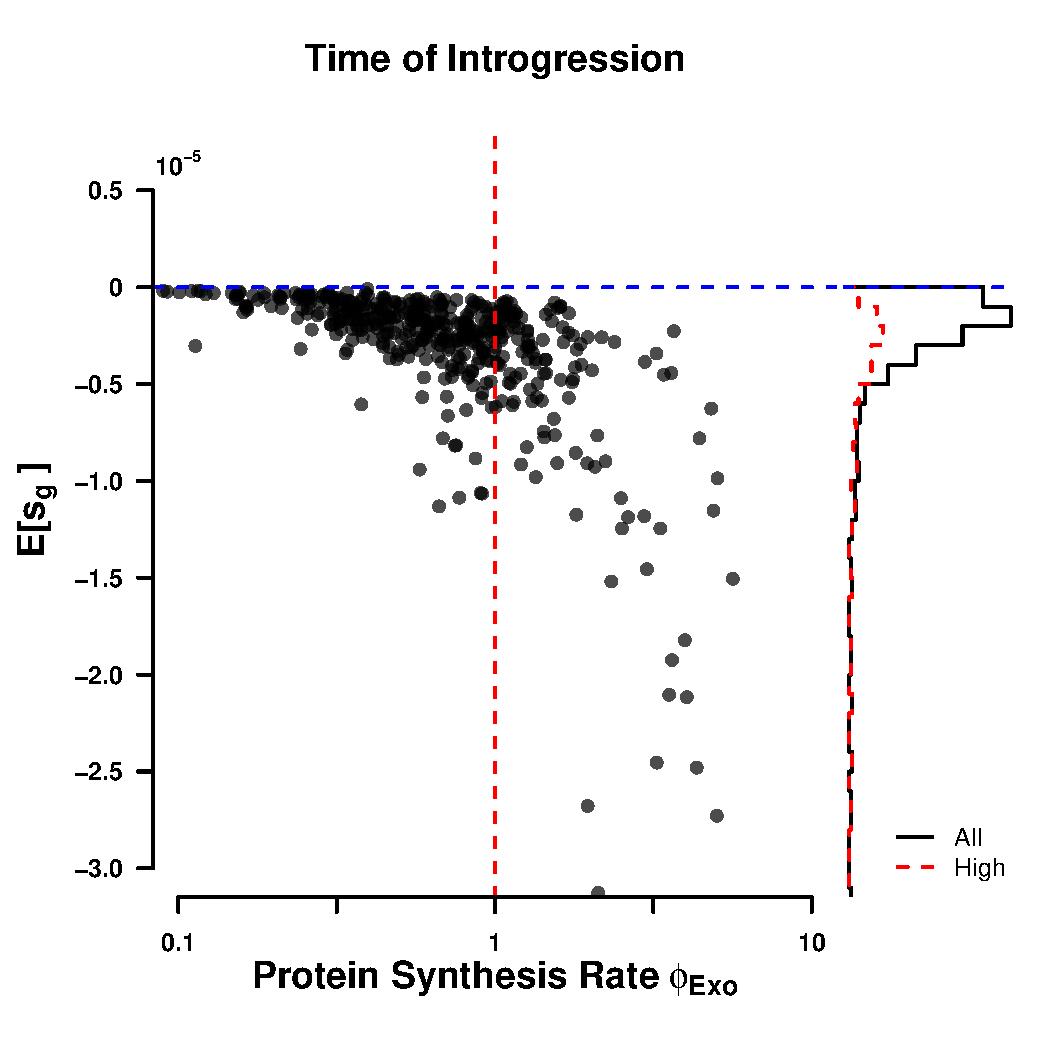
\includegraphics[width=.45\textwidth]{ch3/fitness_difference_gos_kappa1.pdf}
    \end{subfigure}
    \begin{subfigure}
        \centering
        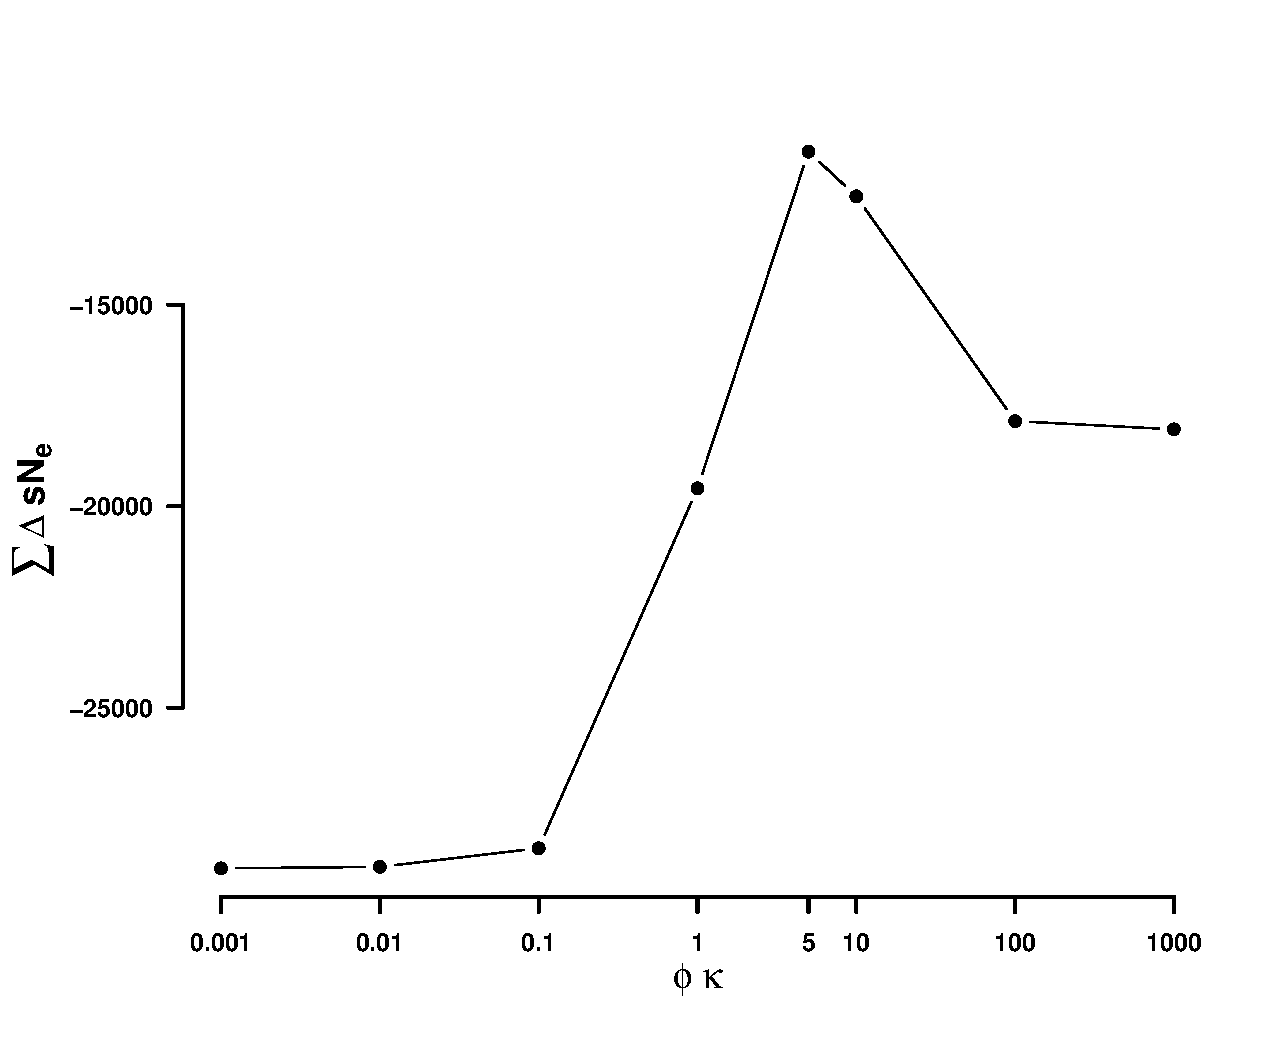
\includegraphics[width=.45\textwidth]{ch3/fitness_phi_scaling_gos.pdf}
    \end{subfigure}
    \caption{Suppl Fig: Fitness burden (left) without scaling of $\phi$, and change of total fitness burden with scaling $\kappa$}
    \label{fig:sne_scaling}
\end{figure}

\begin{figure}[H]
     \centering
	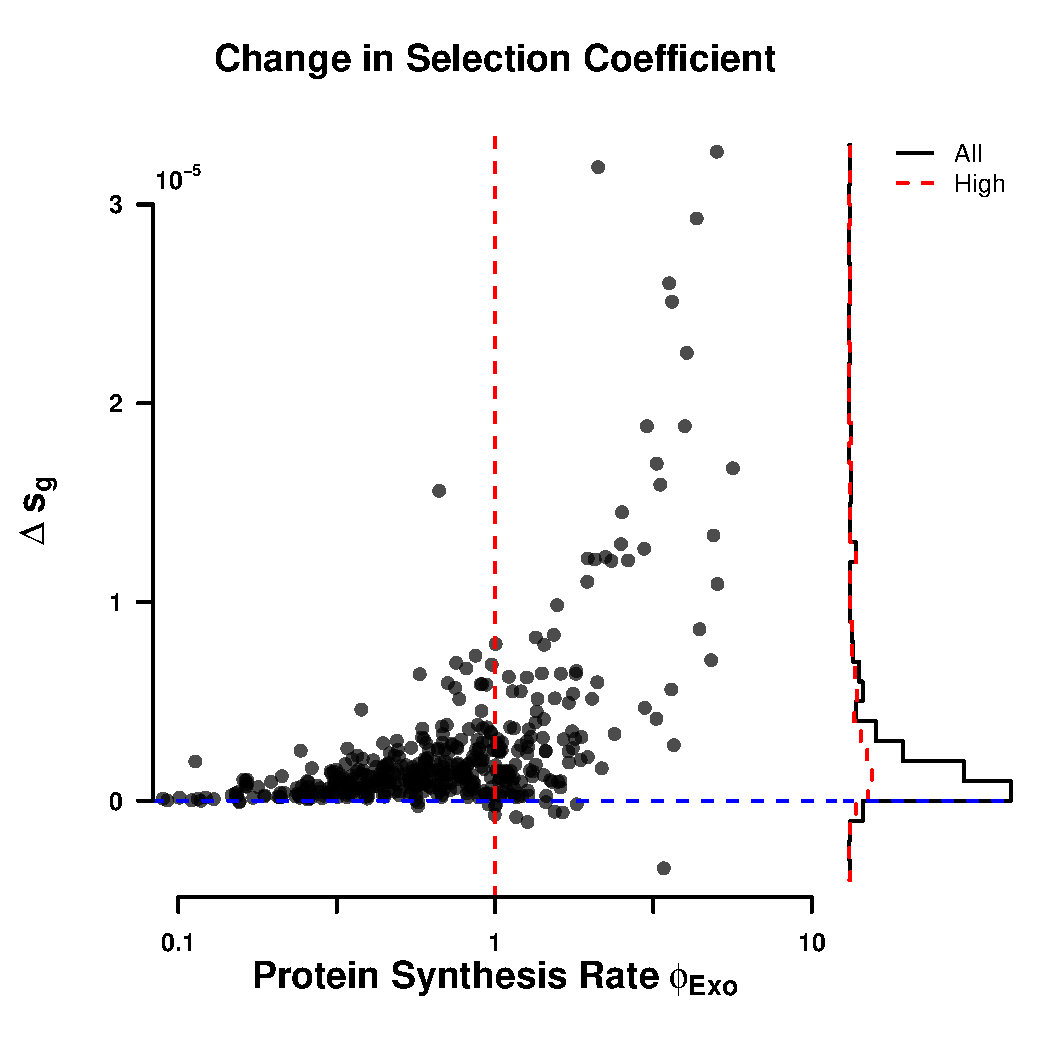
\includegraphics[width=.5\textwidth]{ch3/adaptation_total.pdf}
	\caption{Total amount of adaptation between time of introgression and now}
	\label{fig:adapt_tot}
\end{figure}

\clearpage
\begin{figure}[H]
     \centering
	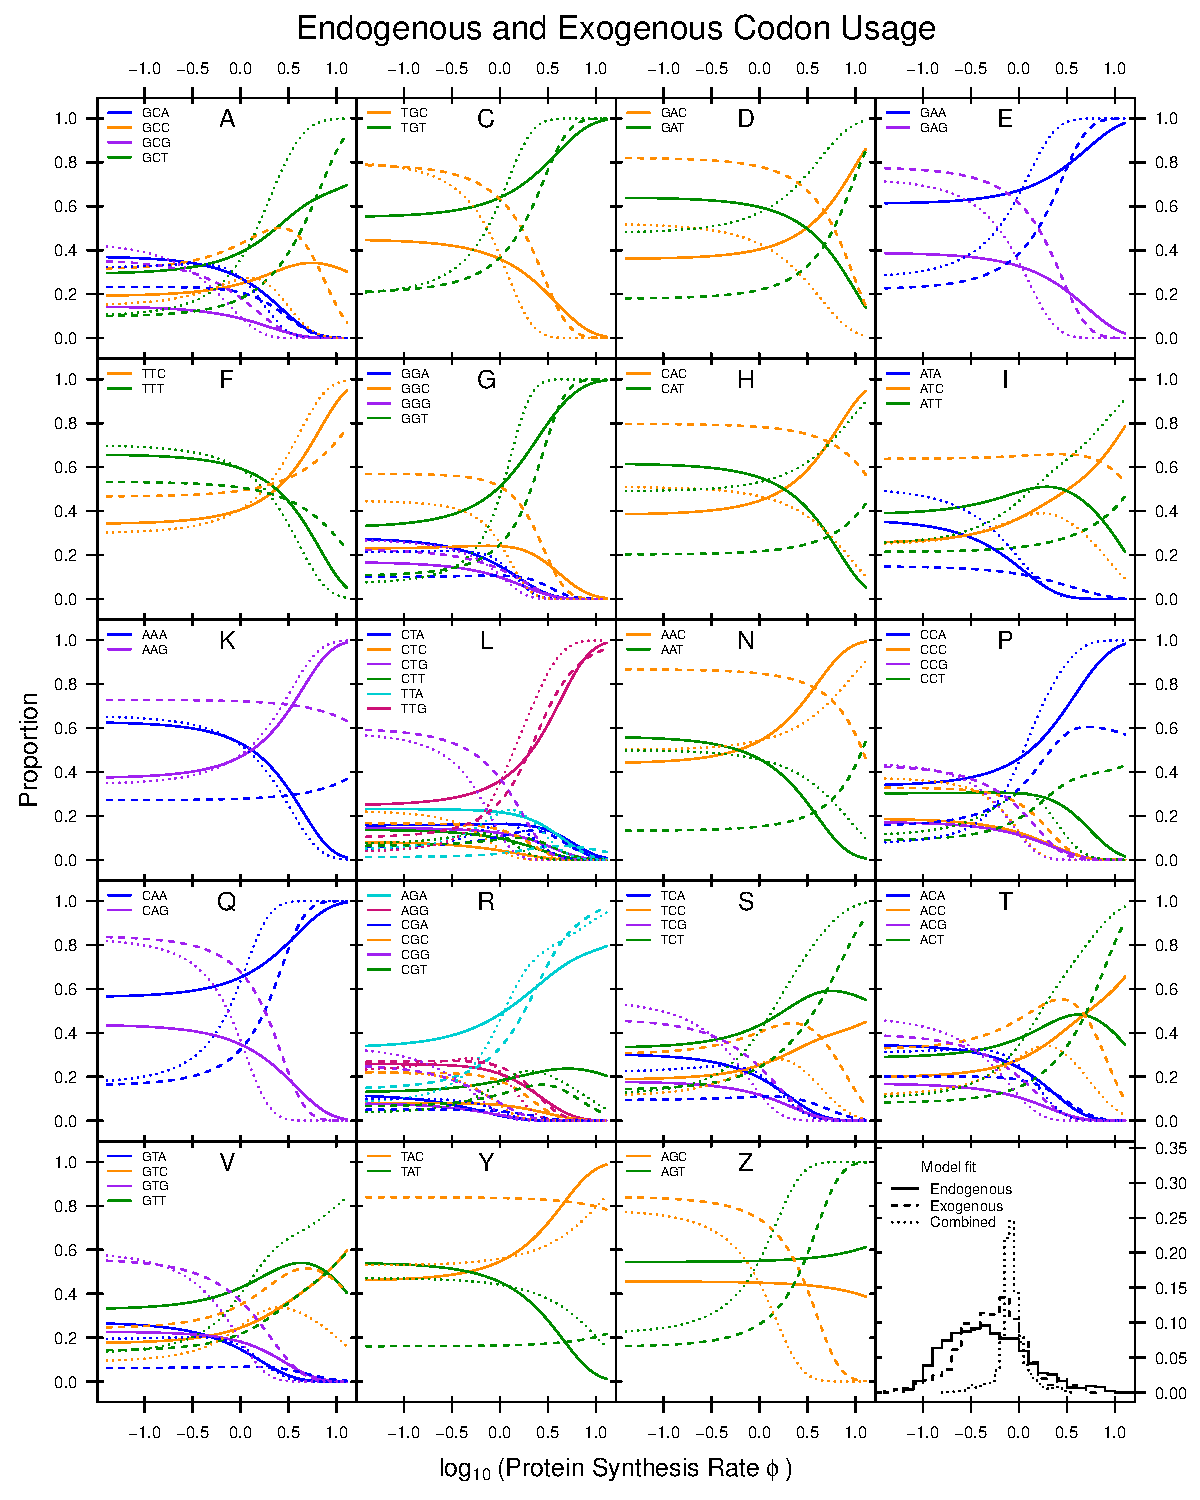
\includegraphics[width=\textwidth]{ch3/CUB_cleft_main.pdf}
	\caption{Suppl Fig}
	\label{fig:cub_all_sets}
\end{figure}

\end{document}

    \chapter{Phylogenetic model of stabilizing selection is more informative about site specific selection than extrapolation from laboratory estimates} 
\label{ch:phylogeny}

\clearpage
\pagebreak

This chapter is a lightly revised version of a paper to be submitted to Genome Biology and Evolution and co-authored with Michael A. Gilchrist and Brian C. O'Meara.\\
\newline
\newline
C. Landerer, B.C. O'Meara, M.A. Gilchrist, Decomposing mutation and selection to identify mismatched codon usage

\section{Abstract}
%\begin{center}\textbf{Abstract}\end{center}
Here we examine the adequacy of experimentally inferred site specific selection for amino acids to inform phylogenetic inferences of sequence evolution.
Previous work has shown that laboratory estimates of selection can improve model fit but did not assess their adequacy.
We assess the adequacy of experimentally inferred site specific selection using DMS to inform phylogenetic models.
We use the $\beta$-lactamse TEM for which empirical estimates of site specific selection on amino acids are readily available.
We compare our results to \selac, a new phylogenetic model of stabilizing selection.
Using simulations to assess model adequacy, we find that experimentally inferred selection does not adequately reflect evolution in the wild.
In contrast, \selac improves model fit over models informed by experimentally inferred selection and provides higher model adequacy.
We demonstrate the capability of \selac by estimating site specific genetic load of the observed TEM variants.

\newpage

\section{Introduction}

Numerous attempts to incorporate selection into phylogenetic models have been made.
Early models focused on the influence of selection on the substitution rate and fixation probability between a resident and a mutant introduced into a population\citep{GoldmanAndYang1994, MuseAndGaut1994, thorne1996}.
These models however, lack site specific equilibrium frequencies.
The importance of site specific equilibrium frequencies has long been noted \citep{felsenstein1981, gojobori1983}.
\citet{HalpernAndBruno1998} first introduced a model to incorporate site specific equilibrium frequencies of amino acids.
However, they had to concede that their model was too parameter rich and therefore intractable for biological data sets without additional simplifying assumptions.
More recent models incorporating site specific equilibrium frequencies still require a large number of parameter to be estimated from the sequence data \citep{LartillotAndPhilippe2004,le2008,wang2008,holder2008,wu2013,tamuri2014}.
Other approaches treat site specific selection as a random effect \citep{rodrigue2010,rodrigue2013,rodrigue2014}.
A full parameterization of site specific equilibrium frequencies for amino acids requires $19\times N$ parameters where $N$ is the length of the sequence in amino acids.
It is therefore an attractive option to utilize laboratory experiments to empirically estimate site specific strength of selection on amino acids and infer their equilibrium frequencies \citep{bloom2014, thyagarajan2014, bloom2017}.

Incorporating empirical estimates of site specific strength of selection on amino acids has important advantages.
Individual amino acid site along the protein show differences in evolutionary rates, and strong preferences for amino acids \citep{HalpernAndBruno1998, ashenberg2013, echave2016}.
The usage of site specific selection acknowledges the heterogeneity in selection and amino acid preferences along the protein sequence \citep{hilton2017}.
Empirical estimates of site specific selection reduce the number of parameters that have to be estimated from the data, making it applicable for smaller data sets and allowing for the fitting of more complex models.
There are, however, also shortcomings.
Deep mutation scanning (DMS) has recently been recently used to generate comprehensive site specific estimates of the strength of selection on amino acids \citep{Fowler2014}.
The ability to estimate site specific strength of selection on amino acids allows to estimate site specific amino acid preferences and the genetic load a mutation introduces at a particular site\citep{bloom2014,firnberg2014,stiffler2016}.
The quality of empirical estimates from DMS, however, depends on many factors including the initial library of mutants and the applied selection \citep{FirnbergAndOstermeier2012}.
Mutation libraries have to be extensive and therefore produce a heterogeneous population of competing organisms usually not found in nature.
In addition, estimates of selection can only be obtained for fast growing organisms that can be manipulated under laboratory conditions.
This is a severe limitation of experimentally informed models as many organism can not be cultivated under laboratory conditions or have long generation times.

Even in the cases where empirical estimates of site specific selection on amino acids can be obtained, their applicability for phylogenetic reconstruction is questionable.
In this study, we assess the adequacy of experimentally inferred site specific selection using DMS to inform phylogenetic models and offer an alternative approach to determine site specific selection on amino acids.
We use site specific estimates of selection on amino acids for the $\beta$-lactamase TEM from \citet{stiffler2016}.
We fitted $227$ nucleotide and codon models using IQTree and compared their model fits to site specific models of stabilizing selection with (\phydms, \selacDMS) and without (\selac) experimentally determined site specific selection coefficients on amino acids \citep{nguyen2015,hilton2017,beaulieu2018}.
We find that experimentally inferred selection, while improving model fit, does not adequately reflect observed wild type sequences.
In contrast, \selac \citep{beaulieu2018} a mechanistic phylogenetic model of stabilizing selection rooted in first principles with site specific equilibrium frequencies improves model fit, and better reflects evolution in the wild.
Because \selac assumes stabilizing selection and that the distance of two amino acids in \PC space affects substitution probabilities it is able to infer the optimal amino acid at a site and reduce the number of site specific parameters from $19\times L$ to $L$.

\section{Results}

\subsection{Site Specific Stabilizing Selection on Amino Acids Improves Model Fit}
We compared \phydms \citep{hilton2017} and \selac \citep{beaulieu2018}, models of site specific stabilizing selection on amino acids, to $227$ other codon and nucleotide models.
We fitted all models to 49 observed sequences of the $\beta$-lactamase TEM.
The \phydms and \selac models with site specific selection on amino acids improved model fits by $366$ and $934$ AICc units, respectively, over codon or nucleotide models without site specific selection (Table \ref{tab:AIC}).
In addition, \selac outperformed the experimentally informed model \phydms by $562$ to $568$ AICc units, depending whether site specific selection on amino acids was inferred by \selac or experimentally informed.

\selac utilizes a hierarchical model and estimates 263 site specific parameters, $\sim5\%$ of the $19\times N = 4997$ parameters necessary to fully describe the site specific selection on amino acids.
In contrast, \phydms does not infer any site specific parameters, but utilizes site specific selection on amino acids estimated from deep mutation scanning experiments.
We fixed the optimal amino acid at each site to the experimentally determined one in \selac and refitted the model to the 49 TEM sequences (\selacDMS).
Incorporating site specific selection on amino acids estimated from deep mutation scanning experiments into \selac (\selacDMS) yields a similar AICc value to \selac without that information.
We incorporated the experimentally inferred site specific amino acids by estimating the 

\begin{table}
  \centering
  \caption{Model selection, shown are the three models of stabilizing site specific amino acid selection (\selac, \selacDMS, \phydms) and the best performing codon and nucleotide model. 
  Reported are the log-likelihood ($\log(\Lik)$), the number of parameters estimated $n$ including edge length, AIC, $\Delta$AIC, AICc, and $\Delta$AICc values.
  See Table \ref{tab:AIC} for all models tested.}  
  \begin{tabular}{lrrrrrr}
    Model		& $\log(\Lik)$ & n & AIC & $\Delta$AIC & AICc & $\Delta$AICc\\ \hline 
    \selacDMS 		& -1768 & 111& 3758& 14	& 3760  & 0\\
    \selac		& -1498 & 374& 3744&  0	& 3766  & 6 \\
    \phydms 		& -2061 & 102& 4326& 582& 4328 & 568\\
    SYM+R2 		& -2230 & 102& 4663& 919& 4694 & 934 \\
    GY+F1X4+R2 		& -2243 & 102& 4690& 946& 4821 & 1061 \\
  \end{tabular}
  \label{tab:AIC}
\end{table}

However, \selacDMS is favored by AICc.
This is solely due to a decrease in the number of parameters estimated, as the model log-likelihood ($\log(\Lik)$) worsens from $-1498$ to $-1768$ (Table \ref{tab:AIC}).
$263$ of the $374$ parameters estimated are the discrete optimal amino acid state at each site. 
However, it is unclear if discrete parameters contribute to the Kullback-Leibler divergence like continuous parameters do and have to be penalized like such.
Therefore, the number of parameter for \selac is reported conservatively as the number of unique site patterns in the TEM alignment is only 27 which would yield a total number of $138$ parameters (96 edge length, 15 mutation/selection parameters, and 27 optimal amino acids).
This however would likely be an under estimate of the number of parameters estimated and the true number of parameters remains unclear at this point due to the inherent non-independence of the underlying data and the discrete nature of the optimized parameters.

\singlespacing
\begin{figure}[H]
     \centering
	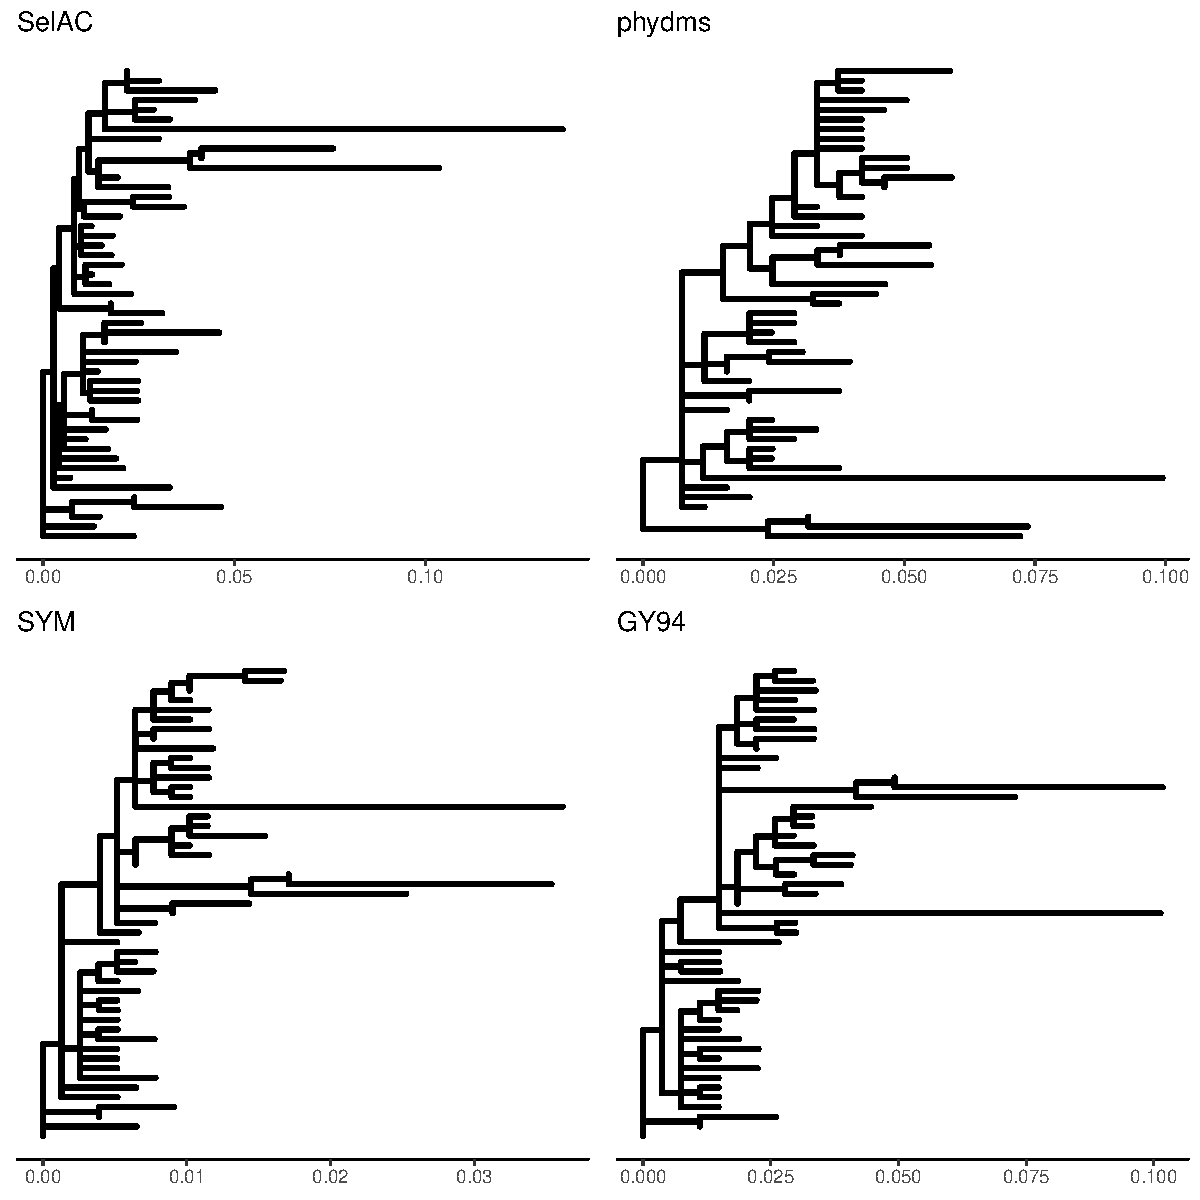
\includegraphics[width=\textwidth]{ch4/phy_TEM2016.pdf}
	\caption{Phylogenies resulting from \selac, \selacDMS, \phydms, and \gy. As \selac is currently to slow for the inference of topologies, the topology for the \selac phylogenies was inferred using the codon model of \citet{KosiolEtAl07}.}
	\label{fig:phylo}
\end{figure}
\doublespacing

We observe differences in the topology between model fits.
The \selac model is currently too slow to estimate the topology, therefore the topology was estimated using the codon model of \citet{KosiolEtAl07}.
At this point, it is therefore unclear if the difference in topology can be attributes to the experimentally inferred selection on amino acids.
We find that the best codon model (\gy) \citep{GoldmanAndYang1994} is outperformed by several nucleotide model e.g. \emph{SYM} \citep{zharkikh1994}.
This could be an indication that negative frequency dependent selection like it is modeled in \gy is not appropriate for TEM \citep{GoldmanAndYang1994,beaulieu2018}.
Figure \ref{fig:phylo} shows that the estimated phylogenetic trees shift from long terminal branches (\selac) to longer internal branches (\phydms).
While the \selac model fit shows $84 \%$ of all evolution happening at the tips, this reduces to $79 \%$ in the \selacDMS model fit, and $77 \%$ in the \phydms and \gy model fits.
All models produce polytomies but their location differs between models.
The largest polytomies appear in the experimentally informed phylogenies of \phydms.
The position of the sequences with the longest branches differ between \selac and \phydms.


\subsection{Laboratory Inferences Inconsistent with Observed Sequences.}
The improved model fits with phydms relative to classical nucleotide and codon models are, however, deceiving.
The site specific selection inferred by DMS is inconsistent with the observed TEM sequences.
We find that the sequence of selectively favored amino acids has only $52 \%$ sequence similarity with the observed consensus sequence (Figure \ref{fig:sim_seqs_cons}).
In addition, assuming the site specific selection estimated by DMS, the observed TEM sequences represent an unexpected high genetic load.
%This is in contrast to the $99 \%$ of sequence similarity with the sequence of selectively favored amino acids estimated by \selac.

\singlespacing
\begin{figure}[H]
     \centering
	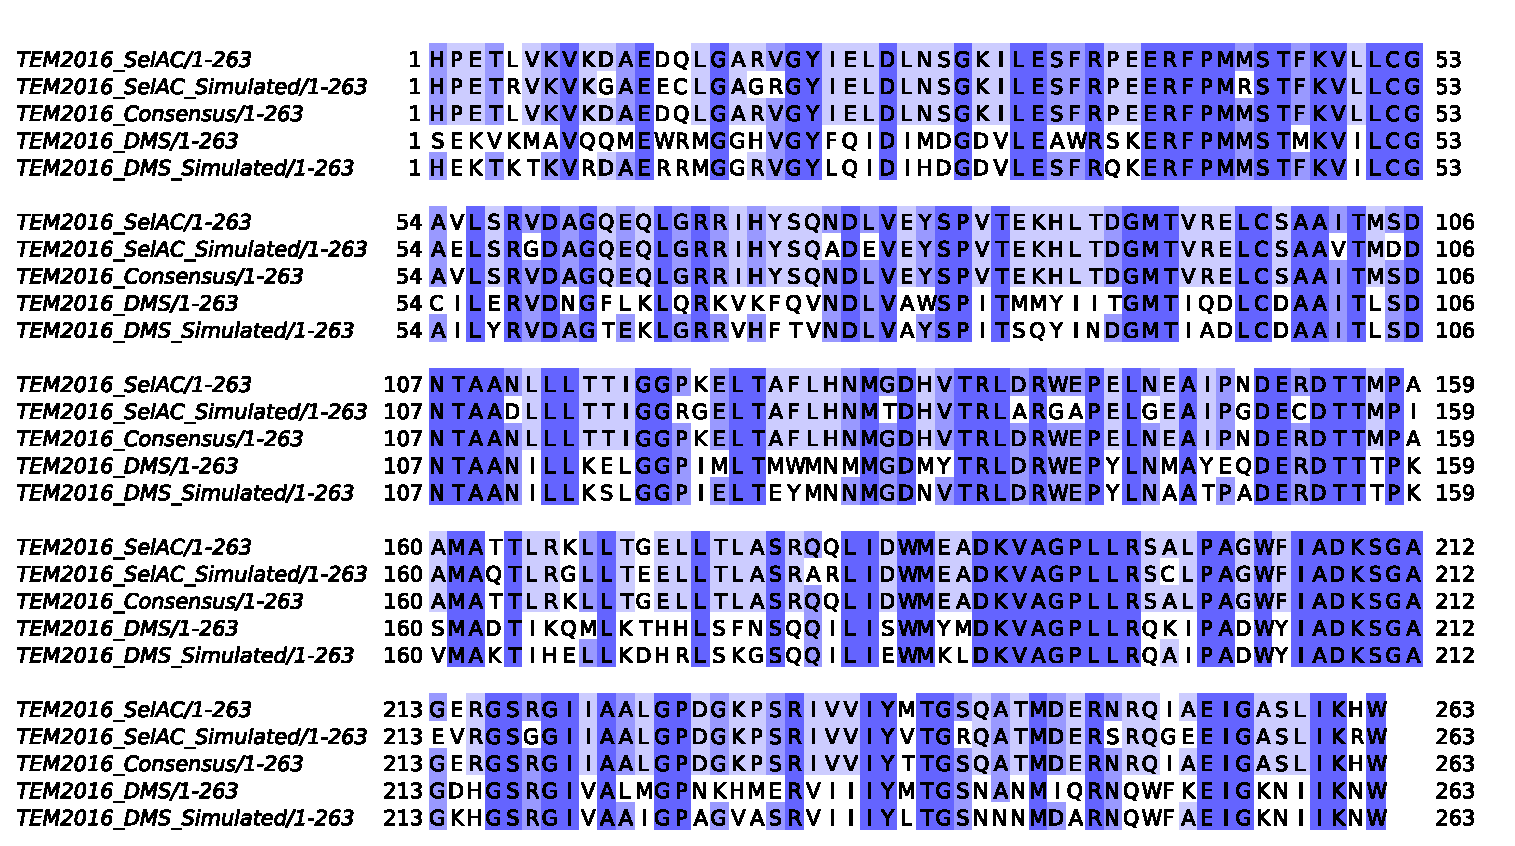
\includegraphics[width=\textwidth]{ch4/seq_simil_all.eps}
	\caption{Alignment of TEM optimal and simulated sequences. Indicated is the percentage identity at each site.}
	\label{fig:sim_seqs_cons}
\end{figure}
\doublespacing

Simulations of codon sequences under the experimentally inferred site specific selection for amino acids reveals that we would not expect to see the observed TEM sequences.
We simulated under a wide range of effective population sizes $N_e$, and find that the experimentally inferred site specific selection is very strong.
With more realistic values of $N_e = 10^7$, we find that the simulated sequences are $62 \%$ similar to the observed consensus sequence (Figure \ref{fig:dms_sim}a).
This is a higher similarity than the observed consensus sequence shows with the sequence of selectively favored amino acids estimated using deep mutation scanning.
Only when $N_e$ is reduced to one individual does drift overpower selection (Figure \ref{fig:dms_sim}b).
The genetic load of the simulated sequences decrease slowly with increasing $N_e$ (Figure \ref{fig:dms_sim}b).
After simulating until the sequences reached $0.1$ expected mutation per site and $N_e = 10^7$ the simulated sequences already show an average genetic load of $0.025$, which is in contrast to the more than $2$ times higher observed load of $0.065$.
Thus it appears unlikely that the observed sequences have evolved under the DMS inferred site specific selection values.


\begin{figure}[h]
    \centering
    \begin{subfigure}
        \centering
        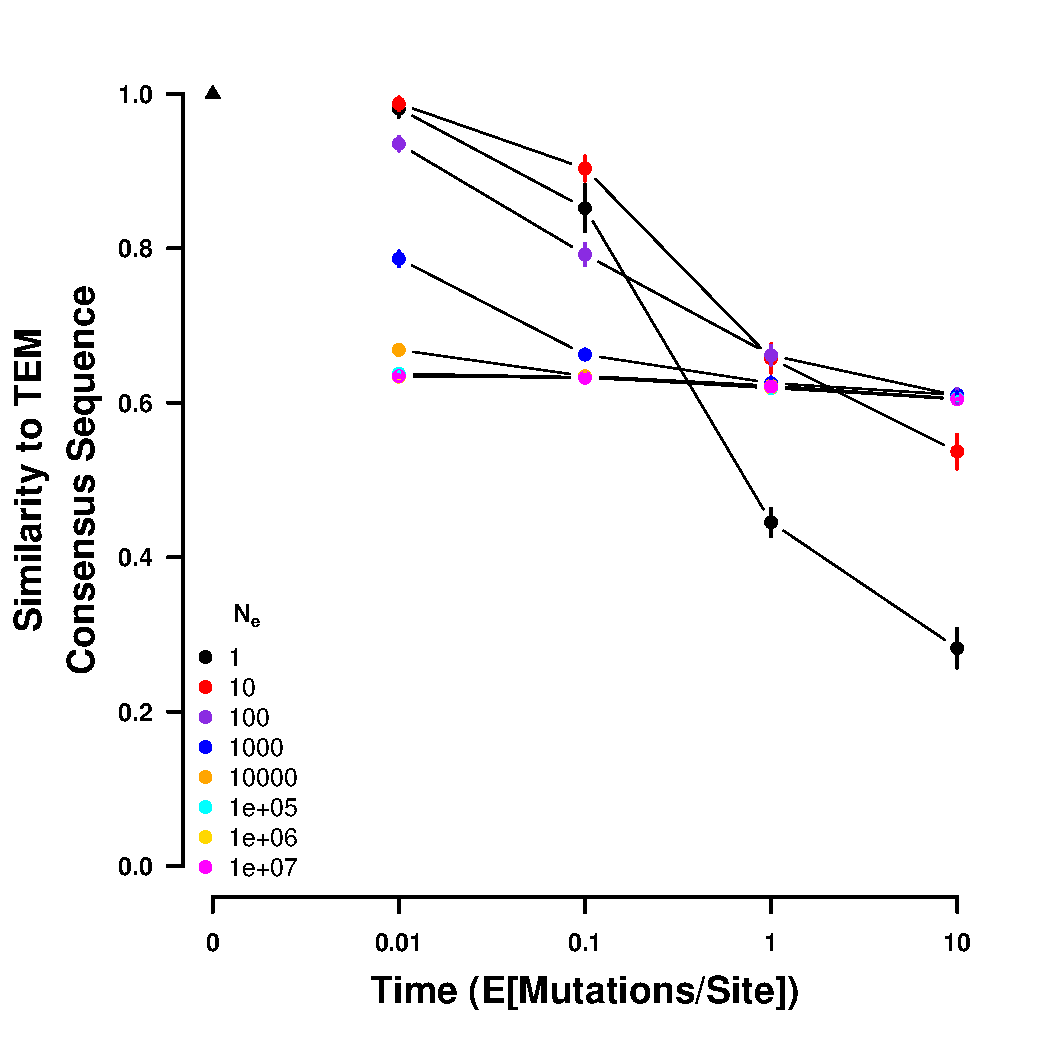
\includegraphics[width=.45\textwidth]{ch4/simulated_dist_time_DMS_ancest.pdf}
    \end{subfigure}
    \begin{subfigure}
        \centering
        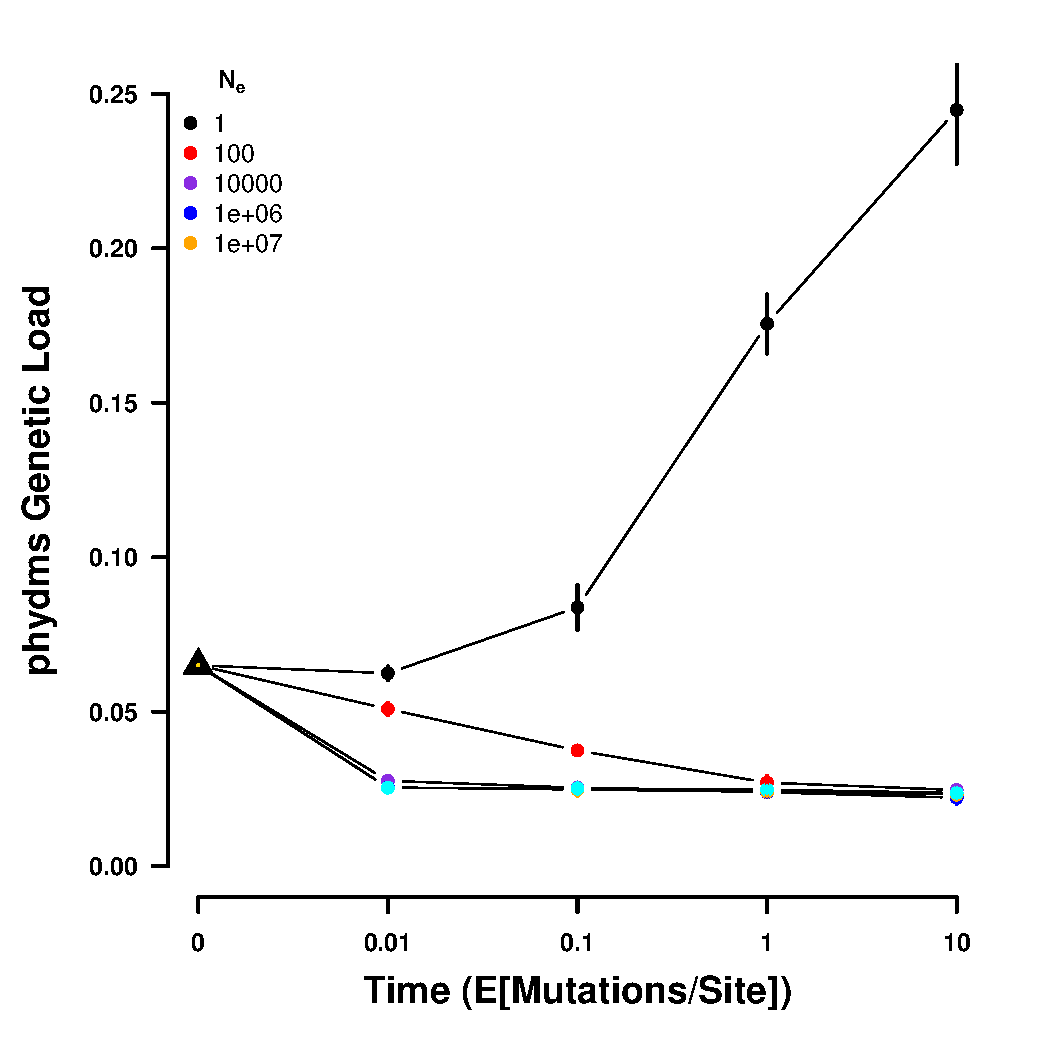
\includegraphics[width=.45\textwidth]{ch4/simulated_gl_time_DMS_ancest.pdf}
    \end{subfigure}
    \caption{Sequences simulated from the ancestral state under the site specific selection on amino acids estimated using deep mutation scanning. 
    (left) Sequence similarity to the observed consensus sequence at various times for a range on values of $N_e$.
    (right) Genetic load of the simulated sequences at various times for a range on values of $N_e$.
    Time is given in number of expected mutations per site, which equals the substitution rate of a neutral mutation.
    Points indicate sample means and vertical bars indicate standard deviations. Initial sequence is the inferred ancestral state of the TEM variants and indicated by a black triangle.}
    \label{fig:dms_sim}
\end{figure}

\subsection{Stabilizing Selection for Optimal Physicochemical Properties Improves Model Adequacy} 
We assessed model adequacy of \selac and find that it better explains the observed TEM sequences than \phydms.
The observed consensus sequence has $99 \%$ sequence similarity with the sequence of selectively favored amino acids estimated by \selac.
Furthermore, assuming the site specific selection estimated by \selac, the observed sequences represent a very small genetic load on the order of $10^{-6}$(Table \ref{tab:selection}, Figure \ref{fig:tem2016_sse}).

We simulated codon sequences forward in time for various length of time, using the \selac inferred site specific selection for amino acids to assess sequence similarity.
% Ancestral starting point
We simulated the evolution of TEM from the inferred ancestral state using a wide range of effective population sizes $N_e$ (Figure \ref{fig:selac_sim}a).
The ancestral state was estimated to be the observed consensus sequence.
As expected, for small $N_e$, simulated sequences drift away from the observed consensus sequence. 
Because of the high similarity between the optimal amino acid sequence estimated by \selac and the observed consensus sequence, the genetic load increases drastically as a result.
Increasing $N_e$ to $10^7$ the simulated sequences reach a sequence similarity of $83 \%$, this is in contrast to the observed average sequence similarity of $98 \%$.

We estimated the total genetic load the sequences represent using the \selac inferred selection on amino acids.
The total genetic load of the simulated sequences averages $9.8\times10^{-6}$ (Figure \ref{fig:selac_sim}b).
The total estimated genetic load of the observed sequences averages $4.2\times 10^{-5}$.
Thus, the simulated sequences show a lower genetic load despite the greater divergence from the observed consensus sequence.

\begin{figure}[h]
    \centering
    \begin{subfigure}
        \centering
        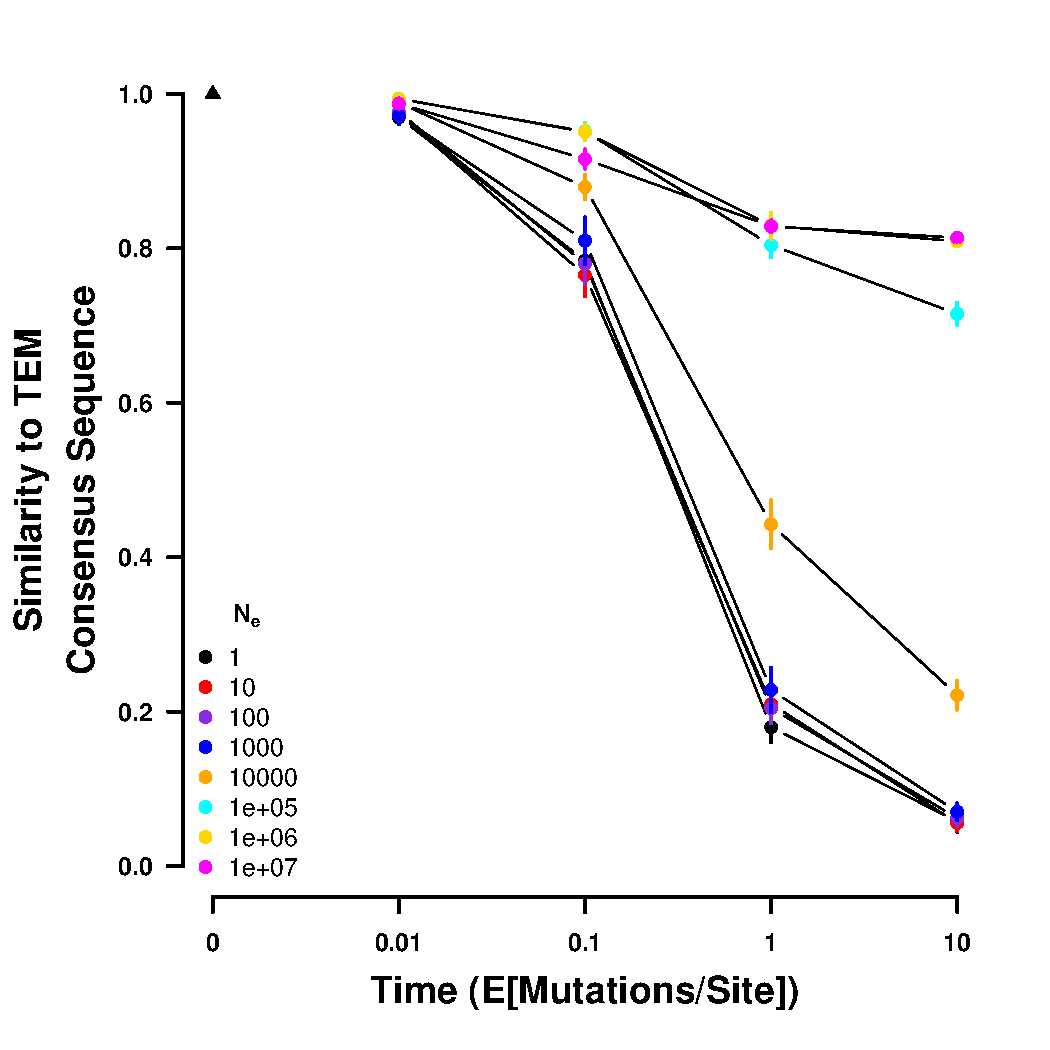
\includegraphics[width=.45\textwidth]{ch4/simulated_dist_time_SELAC_ancest.pdf}
    \end{subfigure}
    \begin{subfigure}
        \centering
        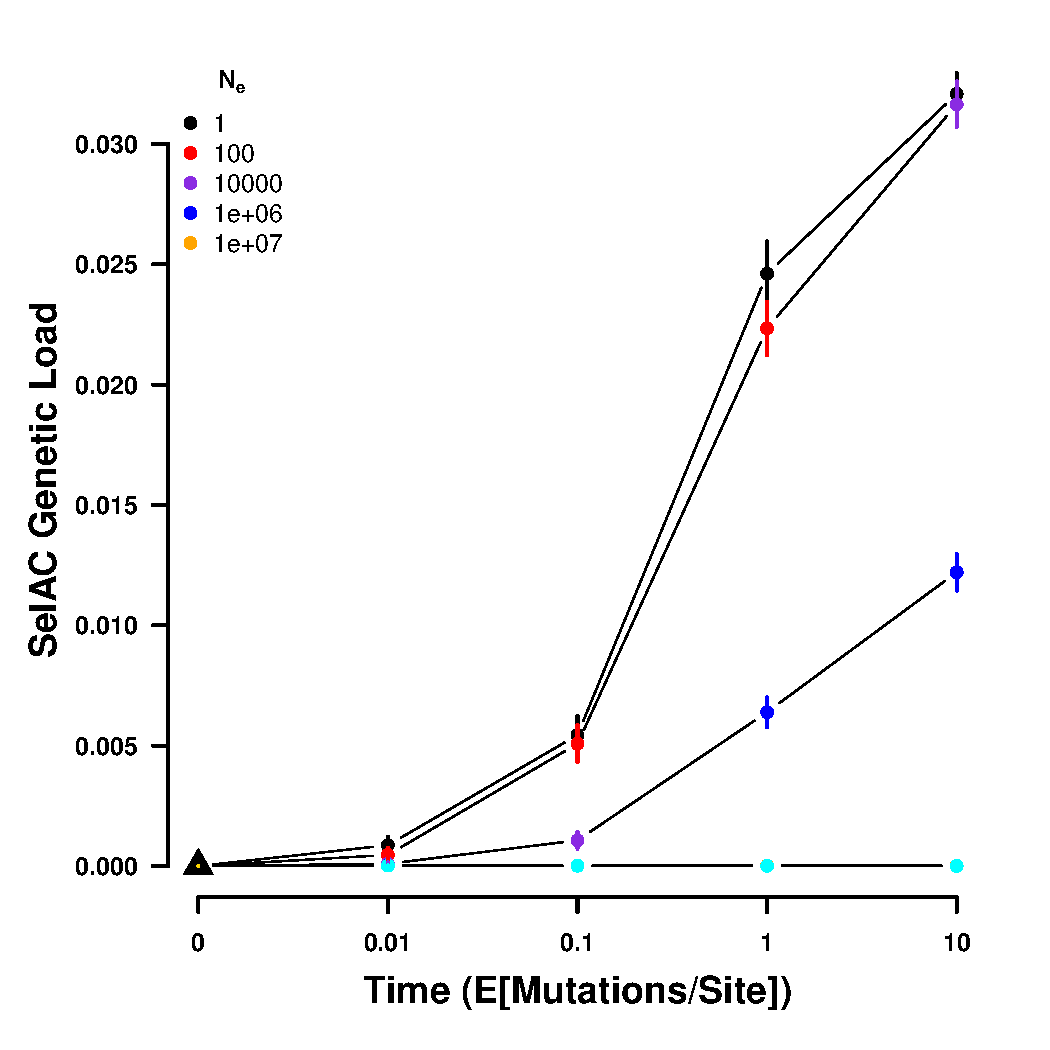
\includegraphics[width=.45\textwidth]{ch4/simulated_gl_time_SELAC_ancest.pdf}
    \end{subfigure}
    \caption{Sequences simulated from the ancestral state under the site specific selection on amino acids estimated using \selac. 
    (left) Sequence similarity to the observed consensus sequence at various times for a range on values of $N_e$.
    (right) Genetic load of the simulated sequences at various times for a range on values of $N_e$.
    Time is given in number of expected mutations per site, which equals the substitution rate of a neutral mutation.
    Points indicate sample means and vertical bars indicate standard deviations. Initial sequence is the inferred ancestral state of the TEM variants and indicated by a black triangle.}
    \label{fig:selac_sim}
\end{figure}

% Random starting point
To further demonstrate the consistency of \selac, we simulated codon sequences over the same period of time using $10$ uniform samples codon sequences with $263$ sites, the same length as the observed TEM variants.
We find that the sequence similarity increases with effective population size $N_e$.
The random sequences start of with a similarity of $\sim6 \%$ which increases with $N_e$ to $\sim28 \%$ (Figure \ref{fig:selac_sim_rand}a).
The same initial sequences under the site specific selection inferred by the deep mutation scanning experiment increase only to $\sim18 \%$ in sequence similarity.



\subsection{Estimating Site Specific Selection on Amino Acids}
\selac allows for the estimation of site specific selection on amino acids and the genetic load of an observed amino acid relative to the inferred optimal amino acid.
Figure \ref{fig:tem2016_sse} and Figure \ref{fig:tem2016_3d} illustrate how the genetic load varies along the TEM sequence.
The region between residue $80$ to $120$ where three consecutive helices are located consist only of selectively favored amino acids and does not show any genetic load. 
The highest genetic load is found in the unstructured regions and the lowest genetic load is found in $\beta$-sheets.
Despite the differences, none show statistical significance.
The largest increase in genetic load is located at the beginning of the last helix.
This strongly contributes to the estimate of similar genetic loads for helices and unstructured regions in the observed TEM sequences (Table \ref{tab:selection}).
However, exclusion of this site as outliers does not produce a significant difference in genetic load between unstructured and helix regions.

The highest efficacy of selection $G$ and the lowest genetic load among the TEM secondary structure features is estimated in the $\beta$-sheet regions.
Residues forming the active and substrate binding site appear to be under the strongest selection, with no accumulated genetic load.
However, we find in one sequence (\textit{Acinetobacter baumannii}, TEM-193) a Lysine, a proton donor, at the proton acceptor site 143 driving the reduced efficacy of selection $G$. 
This is in concordance with the experimental estimates, where proton acceptors are selectively favored.
Again, differences between secondary structure elements are not statistically significant.

\begin{table}
  \centering
  \caption{Efficacy of selection (G) and Genetic Load for TEM and SHV, and separated by secondary structure. G was estimated as a truncated variable with an upper bound of 300.}
  \begin{tabular}{llrrrrr}
    & & & \multicolumn{2}{c}{G} & \multicolumn{2}{c}{Genetic Load $L_i$} \\ 
    Protein & Secondary Structure & \# Residues	& \multicolumn{1}{c}{Mean} & \multicolumn{1}{c}{SE} & \multicolumn{1}{c}{Mean} & \multicolumn{1}{c}{SE} \\ \hline 
    TEM	&		& 263 & 219.3 & 7.5  & $15.9\times10^{-8}$ & $6.5\times10^{-8}$ \\
    &Helix 		& 113 & 206.1 & 12.4 & $17.5\times10^{-8}$ & $13.1\times10^{-8}$ \\
    &$\beta$-Sheet 	&  48 & 238.6 & 15.8 & $ 6.8\times10^{-8}$ & $2.9\times10^{-8}$ \\
    &Unstructured 	& 102 & 224.8 & 11.4 & $18.6\times10^{-8}$ & $8.1\times10^{-8}$ \\
    &Active Sites 	&   5 & 202.6 & 62.2 & $0.01\times10^{-8}$& $0.01\times10^{-8}$ \\ \hline
    
    SHV&		& 263 & 244.9 & 6.8  & $4.0\times10^{-8}$ & $1.9\times10^{-8}$ \\
    &Helix		& 102 & 234.6 & 11.5 & $7.3\times10^{-8}$ & $4.8\times10^{-8}$ \\
    &$\beta$-Sheet 	&  66 & 253.1 & 12.8 & $2.1\times10^{-8}$ & $1.1\times10^{-8}$ \\
    &Unstructured	&  95 & 224.7 & 11.4 & $1.5\times10^{-8}$ & $0.6\times10^{-8}$  \\
    &Active Sites	&   5 & 239.9 & 60.0 & $1.5\times10^{-8}$ & $1.5\times10^{-8}$ \\

  \end{tabular}
  \label{tab:selection}
\end{table}

It was previously proposed that experimentally inferred site specific selection for amino acids can be used to extrapolate the fitness landscape of related proteins \citep{bloom2014, bloom2017}.
We therefore compared the genetic load, the \selac selection parameters of our \selac TEM model fit to a \selac model fit of SHV, and site specific efficacy of selection ($G$).
The genetic load in SHV appears to be lower than in TEM with the exception of residues found in $\beta$-sheets and the active site (Table \ref{tab:selection}).
This is consistent with the elevated efficacy of selection $G$ in SHV.
However, only differences in genetic load in the unstructured regions are significantly different between the TEM and SHV sequences, but only at the $\alpha = 0.05$ significant level ($p = 0.04$).
While the average genetic load across secondary structures is not significantly different, the sites causing increases genetic load differ between SHV and TEM (Figure \ref{fig:shv2016_sse}).
In contrast to TEM, we find the highest genetic load in SHV secondary structure features in the helices (Table \ref{tab:selection}).
We find the highest genetic load in SHV at the end of the first helix.
However, we do find a peak of similar magnitude in the TEM sequence at the end of the first helix, but this peak is overshadowed by increased genetic load at the beginning of the last helix.

We find that site specific efficacy of selection $G$ differs greatly between SHV and TEM ($\rho = 0.12$), despite a similar estimate of $\alpha_G$ describing the distribution of $G$ values (Figure \ref{fig:tem_shv_param_comp}a).
We generally find increased G values in SHV (Table \ref{tab:selection}).
However, non of these increases are statistically significant.
Most \selac selection parameters are very similar between the TEM and the SHV model fit. 
An exception is the weight for the \PC composition property $\alpha_c$ (Figure \ref{fig:tem_shv_param_comp}b).
Furthermore, we find that the sequences of selectively favored amino acids estimated by \selac for TEM and SHV only show $68 \%$ sequence similarity.


\singlespacing
\begin{figure}[H]
     \centering
	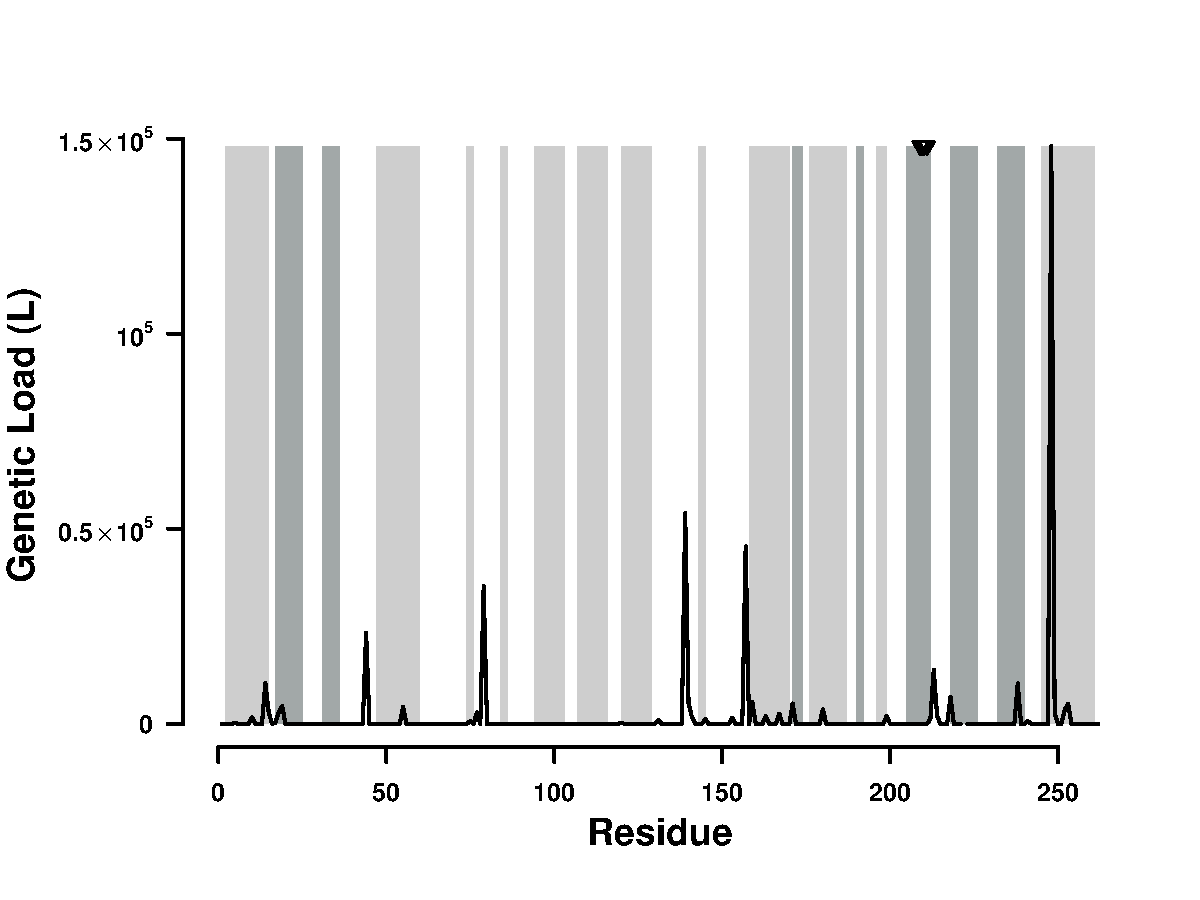
\includegraphics[width=\textwidth]{ch4/GL_slide_TEM2016}
	\caption{Distribution of genetic load in TEM. 
	Average genetic load over all observed TEM variants is indicated by the black line. 
	Light gray bars indicate where helices are found, and dark gray bars indicate $\beta$-sheets.
	The three residues forming the active sites are indicated by three triangles at the top of the plot.}
	\label{fig:tem2016_sse}
\end{figure}
\doublespacing

\section{Discussion}

Here we revisited how well experimental selection estimates from laboratory experiments, specifically deep mutation scanning, explain sequence evolution and compared it to \selac, a novel phylogenetic framework.
Previous work has shown that laboratory estimates of selection can improve model fit over classical approaches like GY94 \citep{bloom2014, bloom2017}.
While our study confirms this notion, we identify important shortcomings of these laboratory estimates.
In contrast, \selac is a more general phylogenetic model of stabilizing selection that does not require costly laboratory estimates of selection and is nevertheless favored by model selection (Table \ref{tab:AIC}).
\selac does not rely on artificially induced selection in the laboratory but is a mechanistic framework rooted in first principles.
It estimates site specific selection on amino acids from the sequence data based on distances between amino acids in \PC space \citep{grantham1974,beaulieu2018}.
This allows \selac to be applied to any set of protein coding sequences, eliminating the need to extrapolate from one homologous gene family to the next (e.g. from TEM to SHV).

While previous work showed the advantages of experimentally informed phylogenetics, they did not assess how adequate the estimated selection reflects observed wild-type sequences.
The low sequence similarity between the observed consensus sequence and the sequence of selectively favored amino acids estimated from deep mutation scanning experiments is evidence for that.
This begs the question how well the experimental selection coefficients represent evolution of sequences in nature.
Deep mutation scanning experiments are performed using a comprehensive library of mutants and a strong artificial selection pressure \citep{FirnbergAndOstermeier2012, Jain2014, FowlerAndFields2014, Fowler2014}.
This results in a very large selection coefficient $s$ and a heterogeneous population of competing individuals unlikely to occur in nature.

The selection pressure imposed during the DMS experiment was limited to ampicillin and focused solely on TEM-1 \citep{stiffler2016}.
However, TEM variants can also confer resistance to a wide range of other antibiotics, including penicillins, cephalosporins, cefotaxime, ceftazidime, or aztreonam \citep{sougakoff1988,sougakoff1989,goussard1991,mabilat1992,chanal1992,brun1994}.
Thus, the inferred selection is biased towards ampicillin and is inconsistent with the observed TEM sequences (Figure \ref{fig:dms_sim}).
This may very well be very appropriate to explore the selection on TEM in a hospital environment but is unlikely to be representative of the selection faced by \ecoli in nature.
%We therefore propose to include a variety of selection pressures if the experimental selection estimates are used for phylogenetic inference.

%TODO:  Lack of repeatability between labs introduces further problems (Firnberg et al 2014 vs. Stifler et al. 2016).

If we assume that the DMS selection coefficients underly the evolution of the observed TEM sequences we are left with two possible explanations for the observed sequences.
First, the sequences are unable to reach a fitness peak, potentially due to a low selection pressure, or not enough time.
Second, the observed TEM sequences are highly maladapted.
Both options seem unlikely.
\ecoli has a large effective population size $N_e$, estimates are on the order of $10^8$ to $10^9$ \citep{OchmanAndWilson1987, hartl1994}.
As new mutations are introduced into a population at a rate proportional to $N_e$, \ecoli can effectively explore the sequence space.
We, therefore, expect the observed sequence variants to be near mutation-selection-drift equilibrium.
This expectation is supported by our simulations in which we observe a higher sequence similarity with the observed TEM consensus sequence and decreased genetic load even with much smaller $N_e$ (Figure \ref{fig:dms_sim}).
Furthermore, previous work showed that the catalytic reaction performed by TEM of penicillin-class antibiotics is close the diffusion limit, making TEM a so-called perfect enzyme \citep{matagne1998}.
The very large effective population size, however, also raises a concern that the population mutation rate of \ecoli $\Theta = 4N_e\mu$ exceeds $0.1$ and violated \selac's weak mutation assumption \citep{deKoning259507}.
If the weak mutation assumption is violated evolution is no longer mutation limited and the time between fixation events increases.

As experimental selection estimates are not readily available for most organsims and proteins, one solution is to extrapolate the estimates to homologous gene families \citep{bloom2014, bloom2017}.
When extrapolating the selection estimates from the $\beta$-lactamase family TEM to the SHV family, the sequence similarity between the observed consensus sequence and the sequence of selectively favored amino acids estimated from deep mutation scanning experiments drops slightly from $52 \% $ to $49 \%$.
In contrast, the site specific efficacy of selection (G) revealed large differences in the site specific selection on amino acids between TEM and SHV.
The mismatched in \PC weights also indicates differences in selection constraints. 
While the polarity of amino acids is of similar importance in TEM and SHV, amino acid composition appears to play a much greater role in SHV than in TEM.
In contrast to the experimental selection estimates, extrapolated from TEM to SHV, the \selac selection estimates are consistent with the observed sequences, e.g. the selectively favored amino acids estimated by \selac shows a high sequence similarity with the observed TEM and SHV consensus sequence ($99 \%$).

While \selac better explains the observed TEM sequences than the experimental estimates of site specific selection on amino acids, it is not without shortcomings itself.
\selac is currently to slow to be used in topology searches, therefore it is unclear if the differences in topology between \phydms and \selac can be attributed to the same inadequacies of experimentally inferred selection.
As the simulation of TEM evolution from he ancestral state under the \selac inferred site specific selection revealed, the formulation of \selac can and should be improved upon.
Starting from the ancestral sequence, the simulated sequences show initial divergence despite stabilizing selection for the optimal amino acid.
While \selac allows for site heterogeneity in selection for amino acids, it still ignores epistasis.
This however, is a shortcoming shared with experimental estimates by deep mutation scanning, as each mutant typically only carries one mutation \citep{FirnbergAndOstermeier2012, Jain2014}.
\selac is a model stabilizing selection, however, not every protein is under stabilizing selection.
TEM plays a role in chemical warfare with conspecifics and other microbes, therefore some sites may be under negative frequency dependent selection.
This potential heterogeneity in selection highlights another shortcoming of \selac.
\selac assumes the same distribution for the efficacy of selection (G) and \PC sensitivities across the whole protein.
However, it is easy to imagine that sites in different secondary structures or at active sites do not share a common distribution.

% TODO: talk about that random sequences still have 30% functionallity under selac. Could explain why the  simulation from the ancestral state diverges to ~80 %. Or maybe do we underestimate selection?

As \selac assumes that the fitness of an amino acid at a site declines with its distance in \PC space to the optimal amino acid, the choice of \PC properties becomes important.
In this study, we assumed the \PC properties estimated by \citet{grantham1974} for all sites.
However, a wide range of additional \PC properties of amino acids have been described \citep{Kawashima2008}.
A more optimal choice of \PC properties may be possible as well as the a relaxation of the assumptions that the same properties apply to all sites equally.
Future work will attempt to address these shortcomings, however, \selac's hierarchical model structure and the open-source code base allow researchers to easily address these shortcoming if desired.

In conclusion, experimental estimates of site specific selection on amino acids have to be treated with skepticism and their adequacy should be assessed before using them to inform phylogenetic inferences.
This study was initiated to assess the quality of \selac with the expectation that \selac could be a faster, cheaper, and more readily available alternative to experimentally inferred selection;
specifically in organisms where these experiments are not feasible.
Intuitively one would expect that selection coefficients estimated of mutations in living organisms would provide more information on the evolution of proteins than a model relying on many simplifying assumptions.
As we show in this study, not only can \selac estimate site specific selection on amino acids but our approach is a more adequate description of selection on amino acids in nature than experimental estimates.


\section{Materials and Methods}

\subsection{Phylogenetic Inference and Model selection}

TEM and SHV sequences were obtained from \citet{bloom2017} already aligned.
We however, separated the TEM and SHV sequences into individual alignments.
Experimentally fitness values for TEM were taken from \citet{stiffler2016}.
We followed \citep{bloom2017} to convert the experimental fitness values into site specific equilibrium frequencies for \phydms. 
\phydms (version 2.5.1) was fitted using site specific selection on amino acids estimated from deep mutation scanning experiments from \citet{stiffler2016} and python (version 3.6).

\selac (version 1.6.1) was fitted to the TEM alignment using R (version 3.4.1) \citep{rcore} with and without site specific selection on amino acids estimated from deep mutation scanning experiments.
We assumed the \PC properties estimated by \citet{grantham1974}.
We chose the constraint free  general unrestricted model \citep{yang1994} as mutation model .
All other models were fitted using IQTree \citep{nguyen2015}.

We report each model's $\log(\Lik)$, AIC, and  AICc. 
Models were selected based on the AICc values.

\subsection{Sequence Simulation}

Sequences were simulated by stochastic simulations using a Gillespie algorithm \citep{gillespie1976} that was model independent.
The simulation followed \citet{SellaAndHirsh2005} to calculate fixation probabilities.
The fitness values were estimated using \selac or experimentally inferred.
We chose the fitness values of the highest concentration (2500 $\mu g/mL$) treatment of ampicillin for our comparison.
We modified the experimental fitness such that the amino acid with the highest fitness at each site has a value of one.
Mutation rates were taken from the \selac or \selacDMS fit.
The initial sequences were either a random sample of 263 codons or the ancestral sequence reconstructed using FastML \citep{fastml} (last accessed: 30.09.2018).
Each sequence was simulated 10 times and we report average genetic load and sequence similarity and the corresponding standard error.
The sequences were sampled at times 0.01, 0.1, 1, and 10 expected mutations per site.

\subsection{Estimating site specific efficacy of selection G}

\selac does not by default estimate site specific values for $G$ but assumes G values follow a gamma distribution \citep{Felsenstein2001}.
Site specific values for $G$ were optimized by fixing all estimated parameters and performing a maximum likelihood search without the usual integration over $G$.
In contrast to \selac that assumes $G$ to be purely positive, we allowed negative values for $G$ and constraint the search to values between $-300$ and $300$.

\subsection{Estimating site specific fitness values $w_i$}

Following \citet{beaulieu2018} $w_i$ is proportional to
\begin{equation}
w_i \propto \exp(-A_0\eta\psi)
\end{equation}
where $A_0$ describes the decline in fitness with each high energy phosphate bond wasted per unit time, and $\psi$ is the protein's production rate.
$\eta$ is the cost/benefit ratio of a protein (see \citep{beaulieu2018} for details). 
However, \selac only estimates a composition parameter $\psi' = A_0\psi N_e$.
$N_e$ describes the effective population size.
\selac assumes $N_e = 5\times 10^6$.
\selac assumes $A_0 = 4 \times 10{-7}$ \citep{gilchrist2007}.
Thus, 
\begin{equation}
\psi = \frac{\psi'}{A_0N_eq}
\end{equation}


\subsection{Model Adequacy}

Model adequacy was assessed by comparing the observed sequences and simulations under the site specific selection inferred by the deep mutation scanning experiment or \selac.
First, similarity between the sequence of selectively favored amino acids and the observed TEM sequences was assessed.
Sequence similarity was measured as the number of differences in the amino acid sequence.
Second, the genetic load of the observed and the simulated sequences was calculated using either the site specific selection inferred by the deep mutation scanning experiment or \selac.

Genetic load was calculated as
\begin{equation}
L_i = \frac{w_{max} - w_i}{w_{max}}
\end{equation}
where $w_{max}$ is the fitness of the sequence of selectively favored amino acids estimated using  the site specific selection inferred by the deep mutation scanning experiment or \selac.
$w_i$ represents the fitness of the $i$th residue.
This the genetic load $L$ of a sequence is given by $L = \sum_{i=1}^n L_i$ where $n$ is the number of amino acids.

\section{Acknowledgments}

This work was supported in part by NSF Award and DEB-1355033 (BCO, MAG, and RZ) with additional support from The University of Tennessee Knoxville. 
CL received support as a Graduate Student Fellow at the National Institute for Mathematical and Biological Synthesis, an Institute sponsored by the National Science Foundation through NSF Award DBI-1300426, with additional support from UTK. 
The authors would like to thank Russel Zaretzki, Jeremy Beaulieu and Alexander Cope for their helpful criticisms and suggestions for this work.




%\bibliographystyle{unsrtnat}
%\bibliography{ecoli}

\clearpage
%\beginsupplement
\section{Appendix: Supplementary Material}

\singlespacing
\begin{longtable}{clrrrrrr}
  \caption{Model selection of 230 models of nucleotide and codon evolution.}\\
  
	No. & Model & LnL & n & AIC & $\Delta$AIC & AICc & $\Delta$AICc \\ \hline
	1 & \selacDMS+G4 & -1768 & 111 & 3758 & 14 & 3760 & 0 \\ 
	2 & \selac+G4 & -1498 & 374 & 3744 & 0 & 3766 & 6 \\ 
	3 & \phydms & -2060.85 & 102 & 4326 & 582 & 4328 & 568 \\ 
	4 & SYM+R2 & -2229.616 & 102 & 4663.232 & 919.232 & 4693.862 & 933.862 \\ 
	5 & TIMe+R2 & -2232.406 & 100 & 4664.811 & 920.811 & 4694.172 & 934.172 \\ 
	6 & TVMe+R2 & -2232.838 & 101 & 4667.677 & 923.677 & 4697.668 & 937.668 \\ 
	7 & TIM3e+R2 & -2234.332 & 100 & 4668.664 & 924.664 & 4698.024 & 938.024 \\ 
	8 & TIM2e+R2 & -2234.381 & 100 & 4668.763 & 924.763 & 4698.123 & 938.123 \\ 
	9 & K3P+R2 & -2235.777 & 99 & 4669.553 & 925.553 & 4698.291 & 938.291 \\ 
	10 & TNe+R2 & -2236.078 & 99 & 4670.155 & 926.155 & 4698.892 & 938.892 \\ 
	11 & SYM+R3 & -2229.616 & 104 & 4667.232 & 923.232 & 4699.162 & 939.162 \\ 
	12 & TIM+F+R2 & -2230.958 & 103 & 4667.915 & 923.915 & 4699.191 & 939.191 \\ 
	13 & TIMe+R3 & -2232.404 & 102 & 4668.808 & 924.808 & 4699.437 & 939.437 \\ 
	14 & GTR+F+R2 & -2228.537 & 105 & 4667.073 & 923.073 & 4699.665 & 939.665 \\ 
	15 & K3Pu+F+R2 & -2232.617 & 102 & 4669.234 & 925.234 & 4699.864 & 939.864 \\ 
	16 & TVM+F+R2 & -2230.105 & 104 & 4668.21 & 924.21 & 4700.14 & 940.14 \\ 
	17 & TVMe+R3 & -2232.838 & 103 & 4671.676 & 927.676 & 4702.952 & 942.952 \\ 
	18 & K2P+R2 & -2239.424 & 98 & 4674.847 & 930.847 & 4702.969 & 942.969 \\ 
	19 & TIM3e+R3 & -2234.332 & 102 & 4672.664 & 928.664 & 4703.293 & 943.293 \\ 
	20 & TIM2e+R3 & -2234.381 & 102 & 4672.762 & 928.762 & 4703.391 & 943.391 \\ 
	21 & TIM3+F+R2 & -2233.064 & 103 & 4672.127 & 928.127 & 4703.403 & 943.403 \\ 
	22 & TIM2+F+R2 & -2233.114 & 103 & 4672.227 & 928.227 & 4703.503 & 943.503 \\ 
	23 & K3P+R3 & -2235.777 & 101 & 4673.553 & 929.553 & 4703.545 & 943.545 \\ 
	24 & TN+F+R2 & -2234.624 & 102 & 4673.249 & 929.249 & 4703.878 & 943.878 \\ 
	25 & TPM3u+F+R2 & -2234.673 & 102 & 4673.347 & 929.347 & 4703.977 & 943.977 \\ 
	26 & TPM3+F+R2 & -2234.674 & 102 & 4673.348 & 929.348 & 4703.978 & 943.978 \\ 
	27 & TPM2u+F+R2 & -2234.681 & 102 & 4673.363 & 929.363 & 4703.993 & 943.993 \\ 
	28 & TPM2+F+R2 & -2234.683 & 102 & 4673.365 & 929.365 & 4703.995 & 943.995 \\ 
	29 & TNe+R3 & -2236.077 & 101 & 4674.155 & 930.155 & 4704.146 & 944.146 \\ 
	30 & TIM+F+R3 & -2230.958 & 105 & 4671.915 & 927.915 & 4704.507 & 944.507 \\ 
	31 & HKY+F+R2 & -2236.266 & 101 & 4674.531 & 930.531 & 4704.522 & 944.522 \\ 
	32 & GTR+F+R3 & -2228.536 & 107 & 4671.073 & 927.073 & 4705.011 & 945.011 \\ 
	33 & K3Pu+F+R3 & -2232.617 & 104 & 4673.234 & 929.234 & 4705.163 & 945.163 \\ 
	34 & TVM+F+R3 & -2230.105 & 106 & 4672.21 & 928.21 & 4705.471 & 945.471 \\ 
	35 & K2P+R3 & -2239.192 & 100 & 4678.384 & 934.384 & 4707.745 & 947.745 \\ 
	36 & TIM3+F+R3 & -2233.063 & 105 & 4676.127 & 932.127 & 4708.718 & 948.718 \\ 
	37 & TIM2+F+R3 & -2233.113 & 105 & 4676.227 & 932.227 & 4708.818 & 948.818 \\ 
	38 & TN+F+R3 & -2234.624 & 104 & 4677.249 & 933.249 & 4709.178 & 949.178 \\ 
	39 & TPM3u+F+R3 & -2234.673 & 104 & 4677.347 & 933.347 & 4709.277 & 949.277 \\ 
	40 & TPM3+F+R3 & -2234.674 & 104 & 4677.348 & 933.348 & 4709.277 & 949.277 \\ 
	41 & TPM2u+F+R3 & -2234.681 & 104 & 4677.363 & 933.363 & 4709.293 & 949.293 \\ 
	42 & TPM2+F+R3 & -2234.682 & 104 & 4677.364 & 933.364 & 4709.294 & 949.294 \\ 
	43 & HKY+F+R3 & -2236.074 & 103 & 4678.148 & 934.148 & 4709.424 & 949.424 \\ 
	44 & SYM+I+G4 & -2243.212 & 102 & 4690.424 & 946.424 & 4721.054 & 961.054 \\ 
	45 & TVMe+I+G4 & -2244.533 & 101 & 4691.066 & 947.066 & 4721.057 & 961.057 \\ 
	46 & TIMe+I+G4 & -2246.457 & 100 & 4692.914 & 948.914 & 4722.275 & 962.275 \\ 
	47 & K3P+I+G4 & -2248.166 & 99 & 4694.332 & 950.332 & 4723.069 & 963.069 \\ 
	48 & TVM+F+I+G4 & -2241.853 & 104 & 4691.707 & 947.707 & 4723.636 & 963.636 \\ 
	49 & TIM3e+I+G4 & -2247.379 & 100 & 4694.758 & 950.758 & 4724.119 & 964.119 \\ 
	50 & K3Pu+F+I+G4 & -2245.156 & 102 & 4694.311 & 950.311 & 4724.941 & 964.941 \\ 
	51 & GTR+F+I+G4 & -2241.484 & 105 & 4692.968 & 948.968 & 4725.559 & 965.559 \\ 
	52 & TIM+F+I+G4 & -2244.418 & 103 & 4694.836 & 950.836 & 4726.112 & 966.112 \\ 
	53 & TPM3u+F+I+G4 & -2246.03 & 102 & 4696.06 & 952.06 & 4726.69 & 966.69 \\ 
	54 & TPM3+F+I+G4 & -2246.069 & 102 & 4696.138 & 952.138 & 4726.768 & 966.768 \\ 
	55 & TIM2e+I+G4 & -2248.934 & 100 & 4697.868 & 953.868 & 4727.228 & 967.228 \\ 
	56 & TNe+I+G4 & -2250.587 & 99 & 4699.174 & 955.174 & 4727.911 & 967.911 \\ 
	57 & TIM3+F+I+G4 & -2245.534 & 103 & 4697.068 & 953.068 & 4728.344 & 968.344 \\ 
	58 & K2P+I+G4 & -2252.181 & 98 & 4700.362 & 956.362 & 4728.484 & 968.484 \\ 
	59 & TPM2u+F+I+G4 & -2247.579 & 102 & 4699.158 & 955.158 & 4729.788 & 969.788 \\ 
	60 & TPM2+F+I+G4 & -2247.685 & 102 & 4699.371 & 955.371 & 4730 & 970 \\ 
	61 & HKY+F+I+G4 & -2249.065 & 101 & 4700.13 & 956.13 & 4730.121 & 970.121 \\ 
	62 & TIM2+F+I+G4 & -2247.009 & 103 & 4700.018 & 956.018 & 4731.294 & 971.294 \\ 
	63 & TN+F+I+G4 & -2248.511 & 102 & 4701.023 & 957.023 & 4731.652 & 971.652 \\ 
	64 & TVMe+I & -2254.804 & 100 & 4709.608 & 965.608 & 4738.968 & 978.968 \\ 
	65 & K3P+I & -2257.72 & 98 & 4711.439 & 967.439 & 4739.561 & 979.561 \\ 
	66 & SYM+I & -2254.11 & 101 & 4710.221 & 966.220 & 4740.212 & 980.212 \\ 
	67 & TIMe+I & -2257.074 & 99 & 4712.149 & 968.149 & 4740.886 & 980.886 \\ 
	68 & TVM+F+I & -2252.157 & 103 & 4710.315 & 966.315 & 4741.591 & 981.591 \\ 
	69 & K3Pu+F+I & -2254.856 & 101 & 4711.712 & 967.712 & 4741.704 & 981.704 \\ 
	70 & TIM3e+I & -2257.796 & 99 & 4713.592 & 969.592 & 4742.33 & 982.33 \\ 
	71 & TPM3+F+I & -2255.771 & 101 & 4713.543 & 969.543 & 4743.534 & 983.534 \\ 
	72 & TPM3u+F+I & -2255.771 & 101 & 4713.543 & 969.543 & 4743.534 & 983.534 \\ 
	73 & K2P+I & -2261.218 & 97 & 4716.436 & 972.436 & 4743.949 & 983.949 \\ 
	74 & GTR+F+I & -2252.067 & 104 & 4712.133 & 968.133 & 4744.063 & 984.063 \\ 
	75 & TIM+F+I & -2254.783 & 102 & 4713.566 & 969.566 & 4744.195 & 984.195 \\ 
	76 & TNe+I & -2260.579 & 98 & 4717.158 & 973.158 & 4745.28 & 985.28 \\ 
	77 & TIM3+F+I & -2255.684 & 102 & 4715.368 & 971.368 & 4745.998 & 985.998 \\ 
	78 & HKY+F+I & -2258.352 & 100 & 4716.703 & 972.703 & 4746.064 & 986.064 \\ 
	79 & TIM2e+I & -2259.878 & 99 & 4717.757 & 973.757 & 4746.494 & 986.494 \\ 
	80 & TVMe+G4 & -2258.853 & 100 & 4717.705 & 973.705 & 4747.066 & 987.066 \\ 
	81 & SYM+G4 & -2257.573 & 101 & 4717.146 & 973.146 & 4747.137 & 987.137 \\ 
	82 & TPM2+F+I & -2257.712 & 101 & 4717.423 & 973.423 & 4747.415 & 987.415 \\ 
	83 & TPM2u+F+I & -2257.712 & 101 & 4717.423 & 973.423 & 4747.415 & 987.415 \\ 
	84 & K3P+G4 & -2261.922 & 98 & 4719.844 & 975.844 & 4747.966 & 987.966 \\ 
	85 & TIMe+G4 & -2260.683 & 99 & 4719.365 & 975.365 & 4748.103 & 988.103 \\ 
	86 & TN+F+I & -2258.28 & 101 & 4718.561 & 974.561 & 4748.552 & 988.552 \\ 
	87 & TIM3e+G4 & -2261.255 & 99 & 4720.51 & 976.51 & 4749.247 & 989.247 \\ 
	88 & TVM+F+G4 & -2256.108 & 103 & 4718.216 & 974.216 & 4749.492 & 989.492 \\ 
	89 & TIM2+F+I & -2257.643 & 102 & 4719.286 & 975.286 & 4749.915 & 989.915 \\ 
	90 & K3Pu+F+G4 & -2258.971 & 101 & 4719.941 & 975.941 & 4749.933 & 989.933 \\ 
	91 & TPM3u+F+G4 & -2259.716 & 101 & 4721.433 & 977.433 & 4751.424 & 991.424 \\ 
	92 & TPM3+F+G4 & -2259.717 & 101 & 4721.434 & 977.434 & 4751.425 & 991.425 \\ 
	93 & GTR+F+G4 & -2255.75 & 104 & 4719.5 & 975.5 & 4751.43 & 991.43 \\ 
	94 & TIM+F+G4 & -2258.638 & 102 & 4721.276 & 977.276 & 4751.906 & 991.906 \\ 
	95 & K2P+G4 & -2265.454 & 97 & 4724.907 & 980.907 & 4752.421 & 992.421 \\ 
	96 & TNe+G4 & -2264.219 & 98 & 4724.437 & 980.437 & 4752.559 & 992.559 \\ 
	97 & TIM3+F+G4 & -2259.366 & 102 & 4722.732 & 978.732 & 4753.361 & 993.361 \\ 
	98 & TIM2e+G4 & -2263.57 & 99 & 4725.141 & 981.141 & 4753.878 & 993.878 \\ 
	99 & JC+R2 & -2266.233 & 97 & 4726.466 & 982.466 & 4753.98 & 993.98 \\ 
	100 & F81+F+R2 & -2262.327 & 100 & 4724.654 & 980.654 & 4754.015 & 994.015 \\ 
	101 & HKY+F+G4 & -2262.499 & 100 & 4724.999 & 980.999 & 4754.359 & 994.359 \\ 
	102 & TPM2+F+G4 & -2261.915 & 101 & 4725.829 & 981.829 & 4755.82 & 995.82 \\ 
	103 & TPM2u+F+G4 & -2261.915 & 101 & 4725.829 & 981.829 & 4755.82 & 995.82 \\ 
	104 & TN+F+G4 & -2262.169 & 101 & 4726.338 & 982.338 & 4756.329 & 996.329 \\ 
	105 & TIM2+F+G4 & -2261.585 & 102 & 4727.17 & 983.17 & 4757.8 & 997.8 \\ 
	106 & F81+F+R3 & -2262.028 & 102 & 4728.056 & 984.056 & 4758.685 & 998.685 \\ 
	107 & JC+R3 & -2265.997 & 99 & 4729.994 & 985.994 & 4758.731 & 998.731 \\ 
	108 & F81+F+I+G4 & -2274.845 & 100 & 4749.69 & 1005.69 & 4779.05 & 1019.05 \\ 
	109 & JC+I+G4 & -2279.318 & 97 & 4752.636 & 1008.636 & 4780.149 & 1020.149 \\ 
	110 & F81+F+I & -2283.56 & 99 & 4765.119 & 1021.119 & 4793.857 & 1033.857 \\ 
	111 & JC+I & -2287.984 & 96 & 4767.968 & 1023.968 & 4794.881 & 1034.881 \\ 
	112 & F81+F+G4 & -2287.834 & 99 & 4773.669 & 1029.669 & 4802.406 & 1042.406 \\ 
	113 & JC+G4 & -2292.095 & 96 & 4776.19 & 1032.19 & 4803.103 & 1043.103 \\ 
	114 & \gy+F1X4+R2 & -2242.963 & 102 & 4689.926 & 945.926 & 4821.251 & 1061.251 \\ 
	115 & MGK+F1X4+R2 & -2243.111 & 102 & 4690.221 & 946.221 & 4821.546 & 1061.546 \\ 
	116 & \gy+F1X4+R3 & -2238.022 & 104 & 4684.043 & 940.043 & 4822.271 & 1062.271 \\ 
	117 & MGK+F3X4+R2 & -2229.923 & 108 & 4675.846 & 931.846 & 4828.729 & 1068.729 \\ 
	118 & \gy+F1X4+I+G4 & -2247.179 & 102 & 4698.359 & 954.359 & 4829.684 & 1069.684 \\ 
	119 & MGK+F1X4+I+G4 & -2247.292 & 102 & 4698.583 & 954.583 & 4829.908 & 1069.908 \\ 
	120 & MGK+F1X4+R3 & -2241.989 & 104 & 4691.978 & 947.978 & 4830.206 & 1070.206 \\ 
	121 & MGK+F3X4+R3 & -2224.78 & 110 & 4669.559 & 925.559 & 4830.217 & 1070.217 \\ 
	122 & \gy+F1X4+G4 & -2251.144 & 101 & 4704.287 & 960.287 & 4832.263 & 1072.263 \\ 
	123 & MGK+F1X4+G4 & -2251.472 & 101 & 4704.944 & 960.944 & 4832.919 & 1072.919 \\ 
	124 & \gy+F3X4+R3 & -2227.048 & 110 & 4674.096 & 930.096 & 4834.754 & 1074.754 \\ 
	125 & \gy+F3X4+R2 & -2233.068 & 108 & 4682.136 & 938.136 & 4835.019 & 1075.019 \\ 
	126 & MGK+F3X4+I+G4 & -2233.539 & 108 & 4683.078 & 939.0781 & 4835.962 & 1075.962 \\ 
	127 & MGK+F3X4+G4 & -2237.512 & 107 & 4689.024 & 945.024 & 4838.134 & 1078.134 \\ 
	128 & \gy+F3X4+I+G4 & -2238.243 & 108 & 4692.485 & 948.485 & 4845.368 & 1085.368 \\ 
	129 & \gy+F3X4+R4 & -2227.106 & 112 & 4678.213 & 934.213 & 4846.96 & 1086.96 \\ 
	130 & \gy+F3X4+G4 & -2242.394 & 107 & 4698.789 & 954.789 & 4847.899 & 1087.899 \\ 
	131 & \gy+F1X4+I & -2260.085 & 101 & 4722.169 & 978.169 & 4850.144 & 1090.144 \\ 
	132 & MGK+F1X4+I & -2260.345 & 101 & 4722.69 & 978.69 & 4850.665 & 1090.665 \\ 
	133 & MGK+F3X4+I & -2246.112 & 107 & 4706.225 & 962.225 & 4855.335 & 1095.335 \\ 
	134 & MG+F1X4+R2 & -2268.482 & 101 & 4738.963 & 994.963 & 4866.938 & 1106.938 \\ 
	135 & \gy+F3X4+I & -2252.532 & 107 & 4719.064 & 975.064 & 4868.174 & 1108.174 \\ 
	136 & MG+F3X4+R2 & -2254.453 & 107 & 4722.906 & 978.906 & 4872.015 & 1112.015 \\ 
	137 & MG+F1X4+I+G4 & -2272.057 & 101 & 4746.113 & 1002.113 & 4874.089 & 1114.089 \\ 
	138 & MG+F1X4+R3 & -2267.523 & 103 & 4741.047 & 997.047 & 4875.789 & 1115.789 \\ 
	139 & MG+F1X4+G4 & -2276.171 & 100 & 4752.342 & 1008.342 & 4877.033 & 1117.033 \\ 
	140 & MG+F3X4+I+G4 & -2257.945 & 107 & 4729.891 & 985.891 & 4879.001 & 1119.001 \\ 
	141 & MG+F3X4+G4 & -2261.949 & 106 & 4735.898 & 991.898 & 4881.309 & 1121.309 \\ 
	142 & MG+F3X4+R3 & -2253.514 & 109 & 4725.027 & 981.027 & 4881.759 & 1121.759 \\ 
	143 & SYM & -2329.878 & 100 & 4859.756 & 1115.756 & 4889.116 & 1129.116 \\ 
	144 & TIMe & -2333.105 & 98 & 4862.21 & 1118.21 & 4890.332 & 1130.332 \\ 
	145 & TIM3e & -2333.481 & 98 & 4862.961 & 1118.961 & 4891.083 & 1131.083 \\ 
	146 & TVMe & -2333.164 & 99 & 4864.328 & 1120.328 & 4893.065 & 1133.065 \\ 
	147 & GTR+F & -2328.404 & 103 & 4862.809 & 1118.809 & 4894.085 & 1134.085 \\ 
	148 & K3P & -2336.391 & 97 & 4866.783 & 1122.783 & 4894.297 & 1134.297 \\ 
	149 & MG+F1X4+I & -2284.946 & 100 & 4769.892 & 1025.892 & 4894.583 & 1134.583 \\ 
	150 & TVM+F & -2330.086 & 102 & 4864.172 & 1120.172 & 4894.802 & 1134.802 \\ 
	151 & TIM+F & -2331.48 & 101 & 4864.96 & 1120.96 & 4894.952 & 1134.952 \\ 
	152 & TNe & -2336.729 & 97 & 4867.458 & 1123.458 & 4894.972 & 1134.972 \\ 
	153 & K3Pu+F & -2333.162 & 100 & 4866.323 & 1122.323 & 4895.684 & 1135.684 \\ 
	154 & TIM3+F & -2331.971 & 101 & 4865.942 & 1121.942 & 4895.934 & 1135.934 \\ 
	155 & TPM3+F & -2333.648 & 100 & 4867.297 & 1123.297 & 4896.657 & 1136.657 \\ 
	156 & TPM3u+F & -2333.648 & 100 & 4867.297 & 1123.297 & 4896.657 & 1136.657 \\ 
	157 & TIM2e & -2336.292 & 98 & 4868.584 & 1124.584 & 4896.706 & 1136.706 \\ 
	158 & MG+F3X4+I & -2270.442 & 106 & 4752.885 & 1008.885 & 4898.295 & 1138.295 \\ 
	159 & K2P & -2340.015 & 96 & 4872.03 & 1128.03 & 4898.943 & 1138.943 \\ 
	160 & TN+F & -2335.102 & 100 & 4870.204 & 1126.204 & 4899.565 & 1139.565 \\ 
	161 & HKY+F & -2336.783 & 99 & 4871.566 & 1127.566 & 4900.303 & 1140.303 \\ 
	162 & TIM2+F & -2334.7 & 101 & 4871.401 & 1127.401 & 4901.392 & 1141.392 \\ 
	163 & TPM2u+F & -2336.381 & 100 & 4872.761 & 1128.761 & 4902.122 & 1142.122 \\ 
	164 & TPM2+F & -2336.381 & 100 & 4872.762 & 1128.762 & 4902.123 & 1142.123 \\ 
	165 & JC & -2366.286 & 95 & 4922.571 & 1178.571 & 4948.892 & 1188.892 \\ 
	166 & F81+F & -2362.554 & 98 & 4921.108 & 1177.108 & 4949.229 & 1189.229 \\ 
	167 & \gy+F1X4 & -2315.788 & 100 & 4831.575 & 1087.575 & 4956.267 & 1196.267 \\ 
	168 & KOSI07+FU+R2 & -2325.725 & 97 & 4845.45 & 1101.45 & 4960.675 & 1200.675 \\ 
	169 & MGK+F1X4 & -2318.048 & 100 & 4836.095 & 1092.095 & 4960.787 & 1200.787 \\ 
	170 & KOSI07+FU+R3 & -2323.063 & 99 & 4844.126 & 1100.126 & 4965.599 & 1205.599 \\ 
	171 & MGK+F3X4 & -2304.357 & 106 & 4820.713 & 1076.713 & 4966.124 & 1206.124 \\ 
	172 & \gy+F3X4 & -2306.17 & 106 & 4824.339 & 1080.339 & 4969.749 & 1209.749 \\ 
	173 & KOSI07+FU+I+G4 & -2335.554 & 97 & 4865.108 & 1121.108 & 4980.332 & 1220.332 \\ 
	174 & KOSI07+FU+G4 & -2339.513 & 96 & 4871.026 & 1127.026 & 4983.218 & 1223.218 \\ 
	175 & KOSI07+F3X4+R2 & -2315.814 & 106 & 4843.627 & 1099.627 & 4989.038 & 1229.038 \\ 
	176 & KOSI07+F3X4+R3 & -2310.509 & 108 & 4837.018 & 1093.018 & 4989.901 & 1229.901 \\ 
	177 & KOSI07+F1X4+R2 & -2333.491 & 100 & 4866.983 & 1122.983 & 4991.674 & 1231.674 \\ 
	178 & KOSI07+F1X4+R3 & -2328.692 & 102 & 4861.383 & 1117.383 & 4992.708 & 1232.708 \\ 
	179 & SCHN05+FU+R2 & -2344.705 & 97 & 4883.411 & 1139.411 & 4998.635 & 1238.635 \\ 
	180 & KOSI07+F1X4+I+G4 & -2337.965 & 100 & 4875.93 & 1131.93 & 5000.621 & 1240.621 \\ 
	181 & KOSI07+F1X4+G4 & -2341.156 & 99 & 4880.312 & 1136.312 & 5001.784 & 1241.784 \\ 
	182 & SCHN05+FU+R3 & -2341.179 & 99 & 4880.358 & 1136.358 & 5001.831 & 1241.831 \\ 
	183 & KOSI07+FU+I & -2349.617 & 96 & 4891.233 & 1147.233 & 5003.426 & 1243.426 \\ 
	184 & KOSI07+F3X4+I+G4 & -2323.767 & 106 & 4859.534 & 1115.534 & 5004.944 & 1244.944 \\ 
	185 & MG+F1X4 & -2342.797 & 99 & 4883.593 & 1139.593 & 5005.065 & 1245.065 \\ 
	186 & KOSI07+F3X4+G4 & -2327.376 & 105 & 4864.751 & 1120.751 & 5006.534 & 1246.534 \\ 
	187 & MG+F3X4 & -2328.539 & 105 & 4867.078 & 1123.078 & 5008.861 & 1248.861 \\ 
	188 & SCHN05+F1X4+R3 & -2340.927 & 102 & 4885.854 & 1141.854 & 5017.179 & 1257.179 \\ 
	189 & KOSI07+F1X4+I & -2349.1 & 99 & 4896.2 & 1152.2 & 5017.672 & 1257.672 \\ 
	190 & SCHN05+F3X4+R3 & -2324.472 & 108 & 4864.944 & 1120.944 & 5017.827 & 1257.827 \\ 
	191 & SCHN05+FU+I+G4 & -2354.523 & 97 & 4903.046 & 1159.046 & 5018.27 & 1258.27 \\ 
	192 & SCHN05+F1X4+R2 & -2348.226 & 100 & 4896.452 & 1152.452 & 5021.143 & 1261.143 \\ 
	193 & SCHN05+F3X4+R2 & -2331.916 & 106 & 4875.833 & 1131.833 & 5021.243 & 1261.243 \\ 
	194 & SCHN05+FU+G4 & -2358.682 & 96 & 4909.365 & 1165.365 & 5021.558 & 1261.558 \\ 
	195 & KOSI07+F3X4+I & -2336.826 & 105 & 4883.653 & 1139.653 & 5025.436 & 1265.436 \\ 
	196 & SCHN05+F1X4+I+G4 & -2351.096 & 100 & 4902.192 & 1158.192 & 5026.883 & 1266.883 \\ 
	197 & SCHN05+F1X4+G4 & -2353.895 & 99 & 4905.79 & 1161.79 & 5027.263 & 1267.263 \\ 
	198 & SCHN05+F1X4+R4 & -2340.593 & 104 & 4889.187 & 1145.187 & 5027.414 & 1267.414 \\ 
	199 & SCHN05+F3X4+R4 & -2324.102 & 110 & 4868.203 & 1124.203 & 5028.861 & 1268.861 \\ 
	200 & SCHN05+F3X4+I+G4 & -2338.345 & 106 & 4888.69 & 1144.69 & 5034.101 & 1274.101 \\ 
	201 & SCHN05+F3X4+G4 & -2341.811 & 105 & 4893.621 & 1149.621 & 5035.404 & 1275.404 \\ 
	202 & SCHN05+FU+I & -2370.471 & 96 & 4932.943 & 1188.943 & 5045.135 & 1285.135 \\ 
	203 & SCHN05+F1X4+I & -2363.696 & 99 & 4925.391 & 1181.391 & 5046.864 & 1286.864 \\ 
	204 & SCHN05+F3X4+I & -2352.81 & 105 & 4915.621 & 1171.621 & 5057.404 & 1297.404 \\ 
	205 & KOSI07+FU & -2394.782 & 95 & 4979.563 & 1235.563 & 5088.785 & 1328.785 \\ 
	206 & KOSI07+F1X4 & -2398.44 & 98 & 4992.88 & 1248.88 & 5111.197 & 1351.197 \\ 
	207 & KOSI07+F3X4 & -2383.159 & 104 & 4974.318 & 1230.318 & 5112.546 & 1352.546 \\ 
	208 & SCHN05+FU & -2419.333 & 95 & 5028.665 & 1284.665 & 5137.887 & 1377.887 \\ 
	209 & SCHN05+F1X4 & -2416.544 & 98 & 5029.088 & 1285.088 & 5147.405 & 1387.405 \\ 
	210 & SCHN05+F3X4 & -2402.838 & 104 & 5013.675 & 1269.675 & 5151.903 & 1391.903 \\ 
	211 & \gy+F+R2 & -2208.59 & 159 & 4735.181 & 991.181 & 5229.161 & 1469.161 \\ 
	212 & \gy+F+G4 & -2217.694 & 158 & 4751.388 & 1007.388 & 5234.504 & 1474.504 \\ 
	213 & \gy+F+I+G4 & -2213.659 & 159 & 4745.319 & 1001.319 & 5239.299 & 1479.299 \\ 
	214 & \gy+F+R3 & -2202.599 & 161 & 4727.198 & 983.198 & 5243.673 & 1483.673 \\ 
	215 & \gy+F+I & -2228.346 & 158 & 4772.691 & 1028.691 & 5255.807 & 1495.807 \\ 
	216 & \gy+F+R4 & -2202.61 & 163 & 4731.219 & 987.219 & 5271.26 & 1511.26 \\ 
	217 & \gy+F & -2282.254 & 157 & 4878.509 & 1134.509 & 5351.004 & 1591.004 \\ 
	218 & KOSI07+F+R2 & -2291.643 & 157 & 4897.286 & 1153.286 & 5369.781 & 1609.781 \\ 
	219 & KOSI07+F+G4 & -2301.662 & 156 & 4915.325 & 1171.325 & 5377.438 & 1617.438 \\ 
	220 & KOSI07+F+I+G4 & -2298.418 & 157 & 4910.835 & 1166.835 & 5383.33 & 1623.33 \\ 
	221 & KOSI07+F+R3 & -2286.723 & 159 & 4891.446 & 1147.446 & 5385.426 & 1625.426 \\ 
	222 & KOSI07+F+I & -2311.78 & 156 & 4935.559 & 1191.559 & 5397.672 & 1637.672 \\ 
	223 & SCHN05+F+R2 & -2310.015 & 157 & 4934.03 & 1190.03 & 5406.525 & 1646.525 \\ 
	224 & SCHN05+F+G4 & -2316.684 & 156 & 4945.369 & 1201.369 & 5407.482 & 1647.482 \\ 
	225 & SCHN05+F+I+G4 & -2313.733 & 157 & 4941.467 & 1197.467 & 5413.962 & 1653.962 \\ 
	226 & SCHN05+F+R3 & -2303.732 & 159 & 4925.463 & 1181.463 & 5419.444 & 1659.444 \\ 
	227 & SCHN05+F+I & -2327.127 & 156 & 4966.254 & 1222.254 & 5428.367 & 1668.367 \\ 
	228 & SCHN05+F+R4 & -2303.45 & 161 & 4928.9 & 1184.9 & 5445.375 & 1685.375 \\ 
	229 & KOSI07+F & -2357.579 & 155 & 5025.157 & 1281.157 & 5477.12 & 1717.12 \\ 
	230 & SCHN05+F & -2379.264 & 155 & 5068.528 & 1324.528 & 5520.491 & 1760.491 \\ 
  \label{tab:AIC_full}
\end{longtable}



\begin{figure}[H]
     \centering
	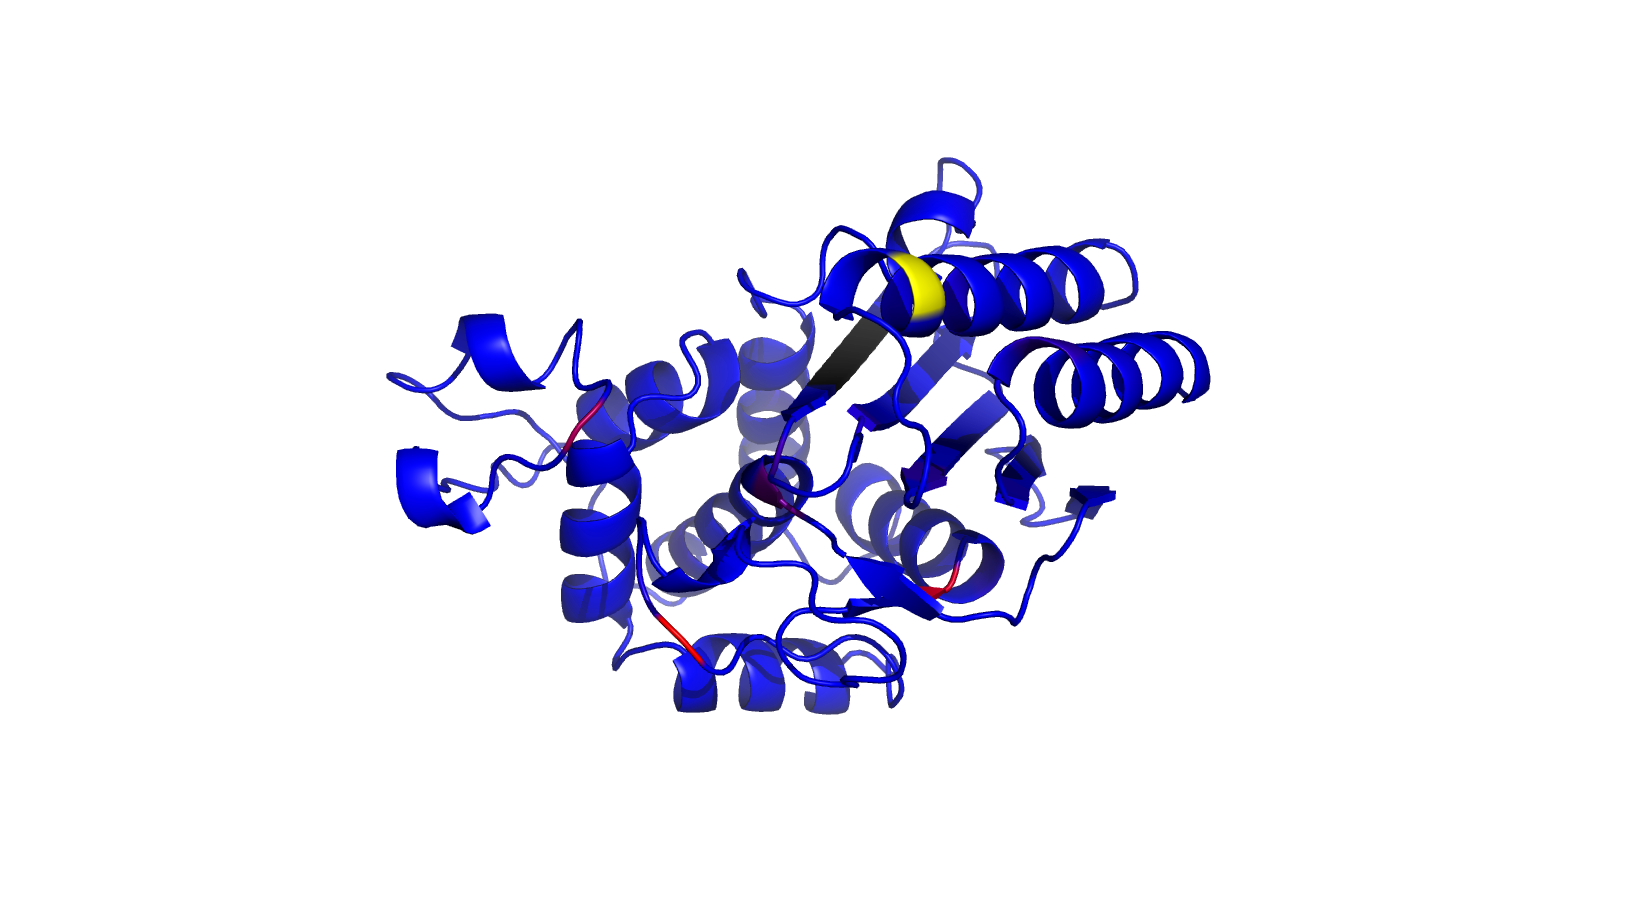
\includegraphics[width=\textwidth]{ch4/1xpb_GL.png}
	\caption{Distribution of genetic load in TEM mapped on its structure (1xpb). 
	Average genetic load over all observed TEM variants is indicated by the color, blue low, red medium, yellow high genetic load. Active site is indicated in black.}
	\label{fig:tem2016_3d}
\end{figure}


\begin{figure}[H]
     \centering
	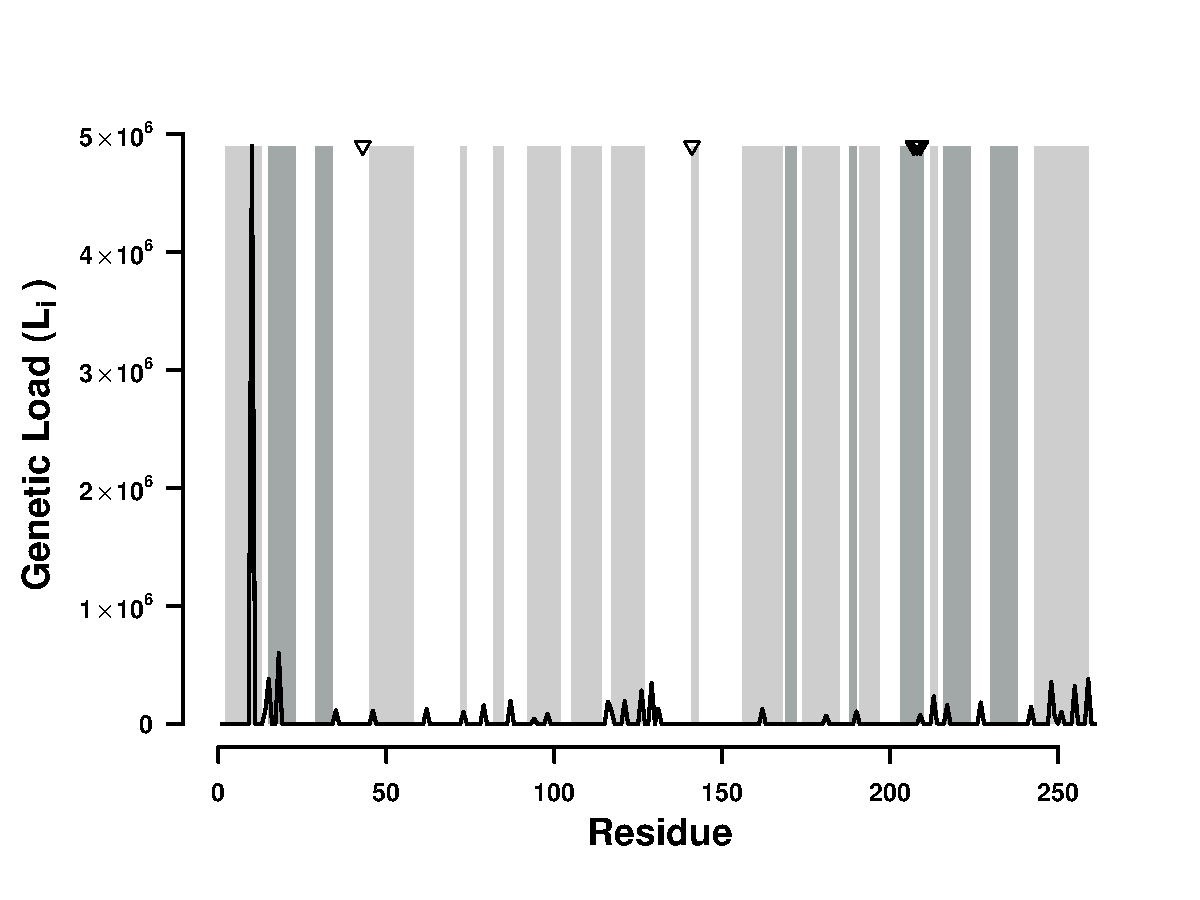
\includegraphics[width=\textwidth]{ch4/GL_slide_SHV2016}
	\caption{Distribution of genetic load in SHV. 
	Average genetic load over all observed SHV variants is indicated by the black line. 
	Light gray bars indicate where helices are found, and dark gray bars indicate $\beta$-sheets.
	The three residues forming the active sites are indicated by three triangles at the top of the plot.}
	\label{fig:shv2016_sse}
\end{figure}

\begin{figure}[h]
    \centering
    \begin{subfigure}
        \centering
        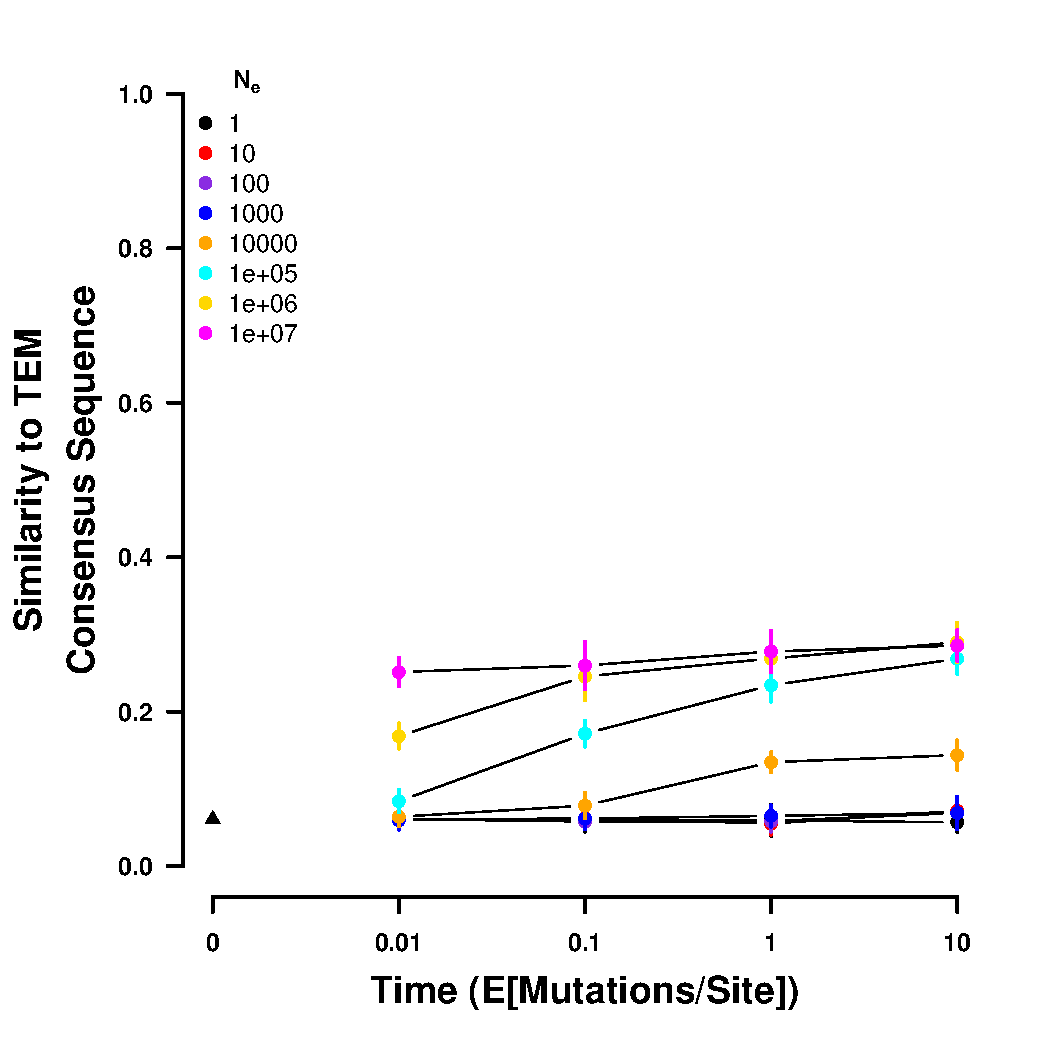
\includegraphics[width=.45\textwidth]{ch4/simulated_dist_time_SELAC_random.pdf}
    \end{subfigure}
    \begin{subfigure}
        \centering
        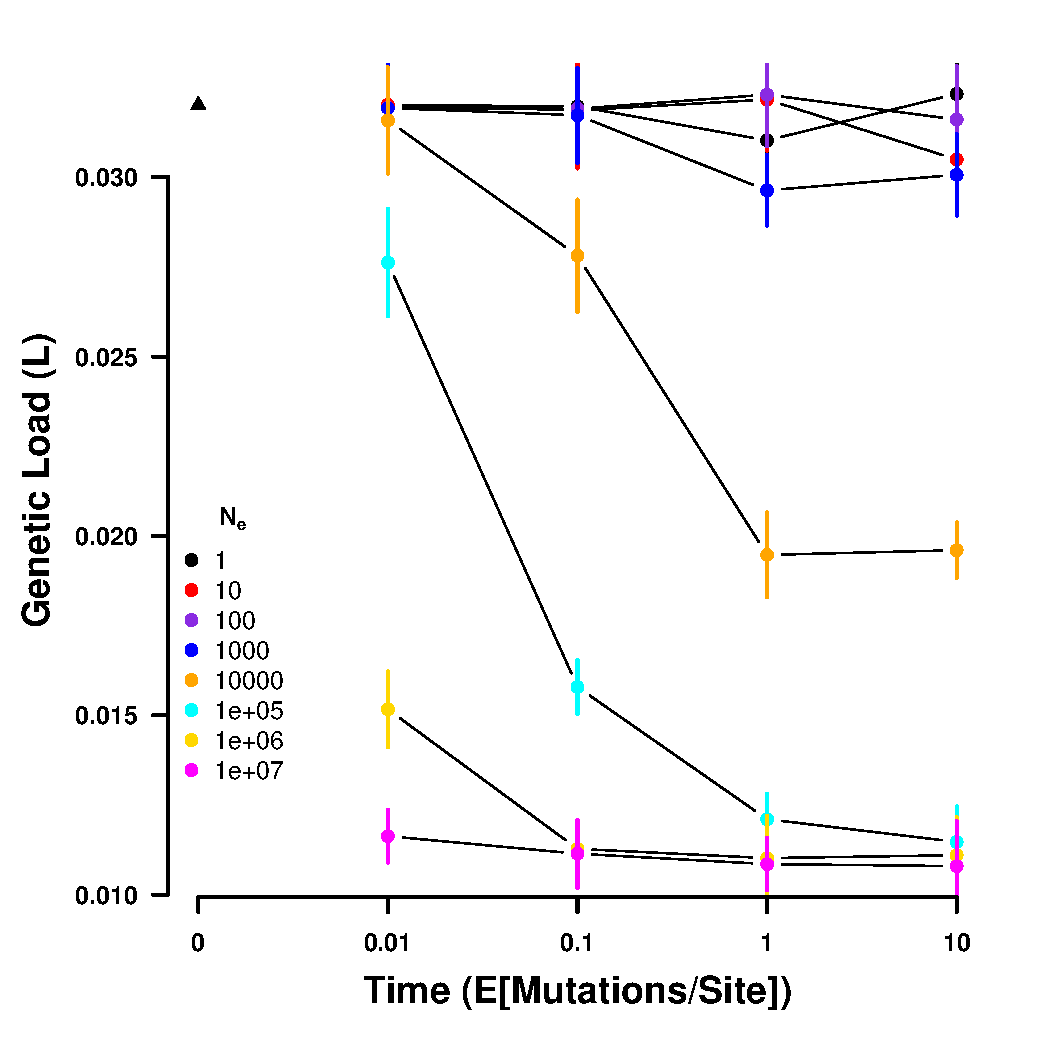
\includegraphics[width=.45\textwidth]{ch4/simulated_gl_time_SELAC_random.pdf}
    \end{subfigure}
    \caption{Sequences simulated from a random codon sequence under the site specific selection on amino acids estimated using \selac. 
    (left) Sequence similarity to the observed consensus sequence at various times for a range on values of $N_e$.
    (right) Genetic load of the simulated sequences at various times for a range on values of $N_e$.
    Time is given in number of expected mutations per site, which equals the substitution rate of a neutral mutation.
    Points indicate sample means and vertical bars indicate standard deviations. Initial sequence is the inferred ancestral state of the TEM variants and indicated by a black triangle.}
    \label{fig:selac_sim_rand}
\end{figure}

\begin{figure}[h]
    \centering
    \begin{subfigure}
        \centering
        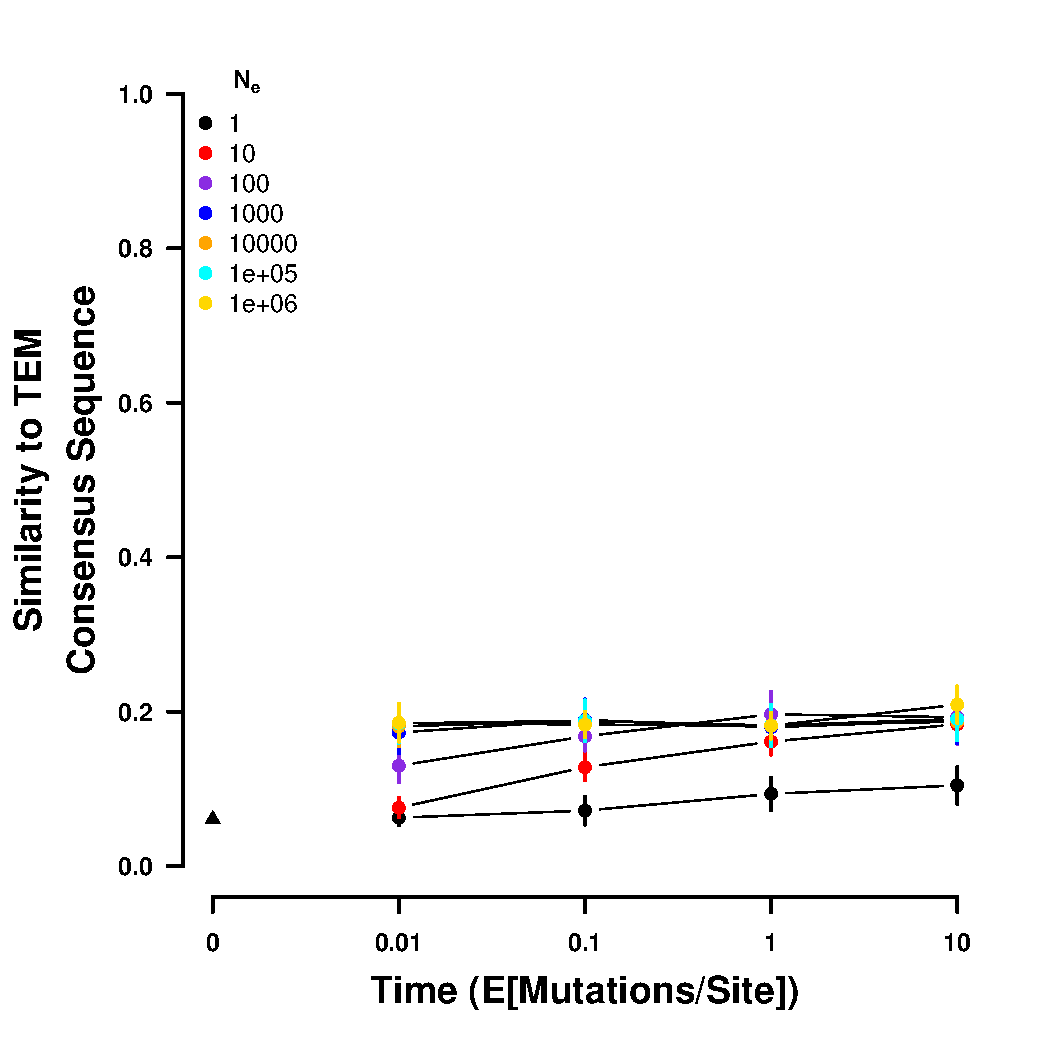
\includegraphics[width=.45\textwidth]{ch4/simulated_dist_time_DMS_random.pdf}
    \end{subfigure}
    \begin{subfigure}
        \centering
        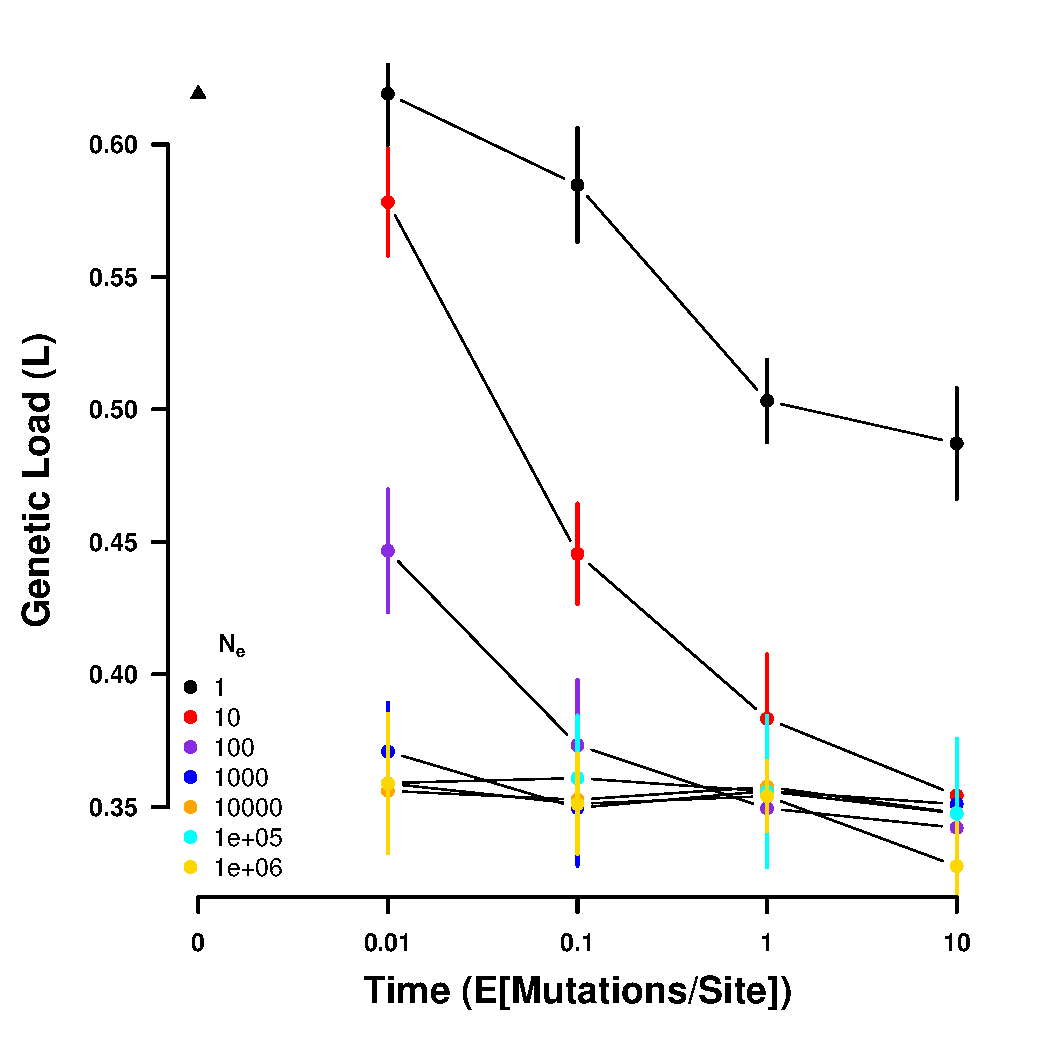
\includegraphics[width=.45\textwidth]{ch4/simulated_gl_time_DMS_random.pdf}
    \end{subfigure}
    \caption{Sequences simulated from a random codon sequence under the site specific selection on amino acids estimated using deep mutation scanning. 
    (left) Sequence similarity to the observed consensus sequence at various times for a range on values of $N_e$.
    (right) Genetic load of the simulated sequences at various times for a range on values of $N_e$.
    Time is given in number of expected mutations per site, which equals the substitution rate of a neutral mutation.
    Points indicate sample means and vertical bars indicate standard deviations. Initial sequence is the inferred ancestral state of the TEM variants and indicated by a black triangle.}
    \label{fig:dms_sim_rand}
\end{figure}

\begin{figure}[h]
    \centering
    \begin{subfigure}
        \centering
        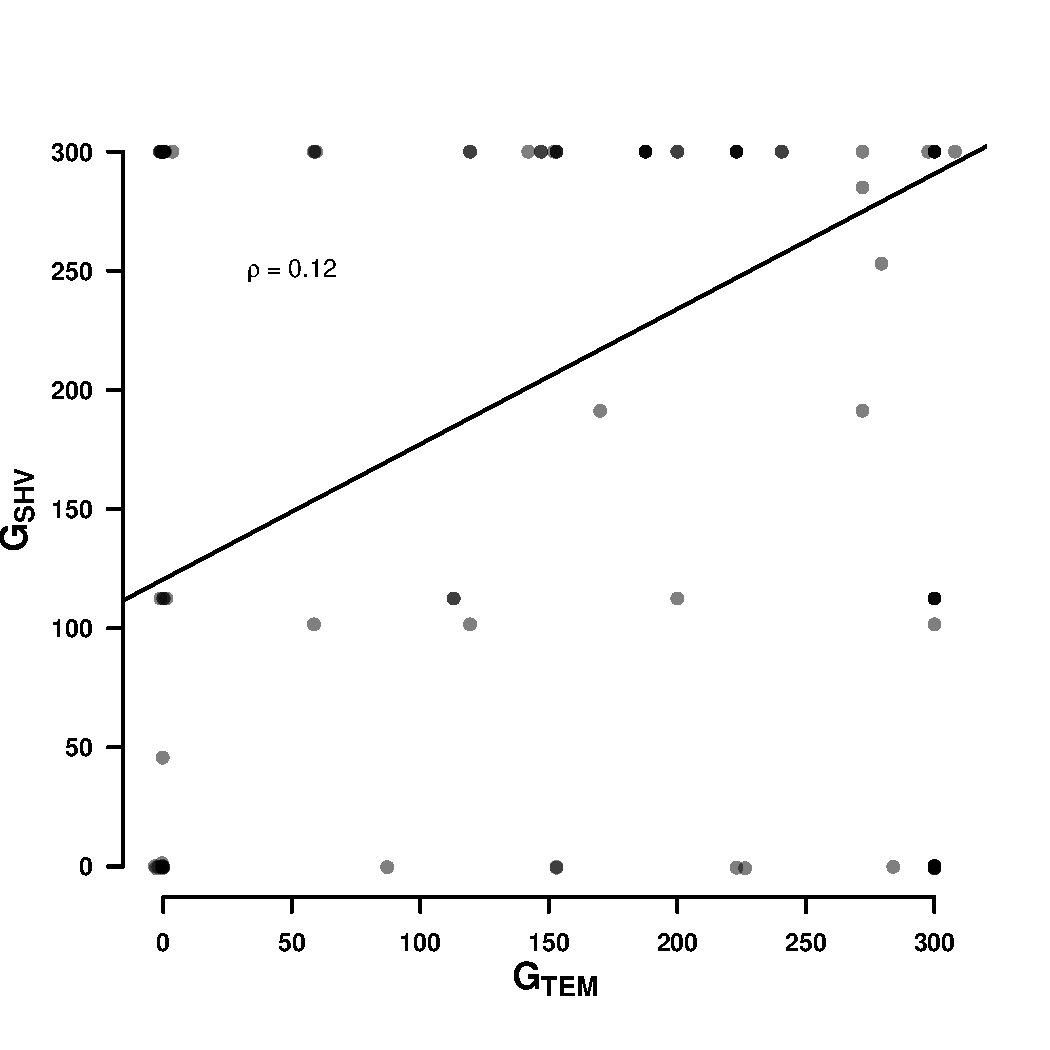
\includegraphics[width=.45\textwidth]{ch4/g_shift_lac.pdf}
    \end{subfigure}
    \begin{subfigure}
        \centering
        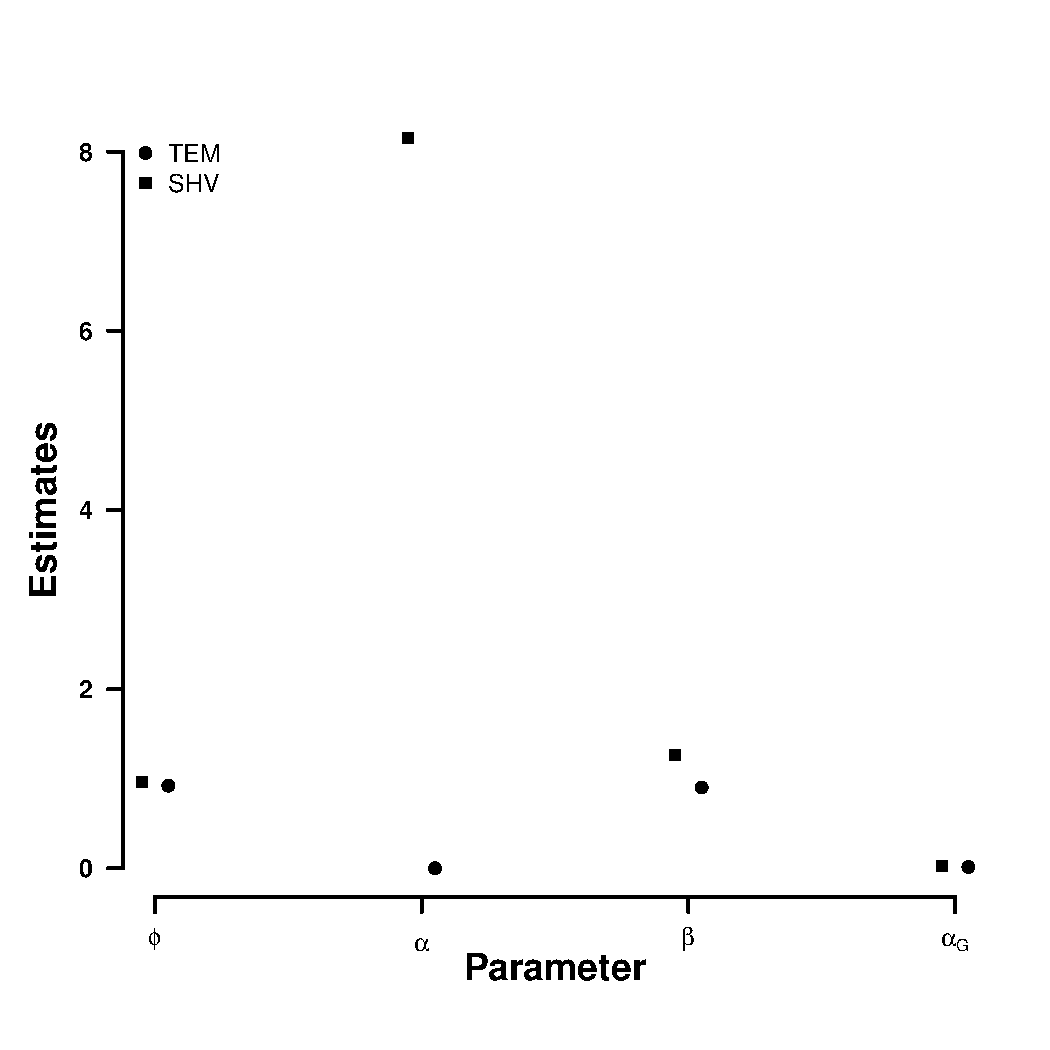
\includegraphics[width=.45\textwidth]{ch4/TEM_SHV_2016_par_comp.pdf}
    \end{subfigure}
    \caption{Comparison of selection related parameters between TEM and SHV. 
    (left) Estimated site specific efficacy of selection $G$. 
    (right) Selection related parameter estimates. 
    Protein functionality production rate $\psi$, \PC weight for amino acid composition $\alpha_c$, \PC weight for amino acid polarity $\alpha_p$, and the parameter describing the distribution of $G$, $\alpha_G$ estimated by \selac.}
    \label{fig:tem_shv_param_comp}
\end{figure}

\doublespacing
    %%%%%%%%%%%%%%%%%%%%%%%%%%%%%%%%%%%%%%%%%%%%%%%%%%%%%%%%%%%%%%%%%%%%%%%%%%%%%%%%%%%%%%%%%%%%%%%%%%%%%
    % BIBLIOGRAPHY
    %%%%%%%%%%%%%%%%%%%%%%%%%%%%%%%%%%%%%%%%%%%%%%%%%%%%%%%%%%%%%%%%%%%%%%%%%%%%%%%%%%%%%%%%%%%%%%%%%%%%%
    \makeBibliographyPage % make the bibliography title page
\newpage

% To make the bibliography, use \utbiblio{#1}{}{} command. Always use "#1" for the first entry. The second entry is your bibliography style, and the third entry is the name of your bibliography file (.bib file extension) 
% bibliography style - recommend using apalike-doi as it hyperlinks DOIs
% Be sure to run BibTeX in order to generate the bibliography correctly.

\utbiblio{#1}{apalike}{bioinfo}

    %%%%%%%%%%%%%%%%%%%%%%%%%%%%%%%%%%%%%%%%%%%%%%%%%%%%%%%%%%%%%%%%%%%%%%%%%%%%%%%%%%%%%%%%%%%%%%%%%%%%%
    % APPENDIX - OPTIONAL - COMMENT OUT IF NOT NEEDED
    %%%%%%%%%%%%%%%%%%%%%%%%%%%%%%%%%%%%%%%%%%%%%%%%%%%%%%%%%%%%%%%%%%%%%%%%%%%%%%%%%%%%%%%%%%%%%%%%%%%%%
    
    \makeAppendixPage{2}   % Input the number of appendices
    \appendix    
    
\section{Summary of Equations}
some text here
\subsection{Cartesian}
some equations here

\subsection{Cylindrical}
some equations also here
    
\section{Summary of Stuff}
some text here
\subsection{More Things}
some equations here

\subsection{Other Aspects}
some equations also here
    %%%%%%%%%%%%%%%%%%%%%%%%%%%%%%%%%%%%%%%%%%%%%%%%%%%%%%%%%%%%%%%%%%%%%%%%%%%%%%%%%%%%%%%%%%%%%%%%%%%%%
    % A VITA IS REQUIRED
    %%%%%%%%%%%%%%%%%%%%%%%%%%%%%%%%%%%%%%%%%%%%%%%%%%%%%%%%%%%%%%%%%%%%%%%%%%%%%%%%%%%%%%%%%%%%%%%%%%%%%
    \addToTOC{Vita}
    \chapter*{Vita} \label{ch:vita}
Premal Shah was born in Akola, India on October 23, 1984.
He was raised in Chennai, India where he graduated high school from GSSJV in 2002. 
In 2006 he graduated from the Anna University at Chennai with a B. Tech. in Industrial Biotechnology. 
He joined the University of Tennessee, Knoxville as a graduate student in the Fall of 2006 and received a Ph. D. in Ecology and Evolutionary Biology in 2011.
Premal will begin working as a postdoctoral research fellow in the Department of Biology at University of Pennsylvania, Philadelphia, PA in June 2011.
\end{document}
